\begin{filecontents}[overwrite]{refs.bib}
@article{roodman2019fast,
  title={Fast and wild: Bootstrap inference in Stata using boottest},
  author={Roodman, David and Nielsen, Morten {\O}rregaard and Webb, Matthew D.},
  journal={The Stata Journal},
  volume={19},
  number={1},
  pages={4--60},
  year={2019},
  publisher={SAGE Publications},
  doi={10.1177/1536867X19830877}
}

@techreport{webb2014reworking,
  title={Reworking wild bootstrap based inference for clustered errors},
  author={Webb, Matthew D.},
  institution={Queen's Economics Department Working Paper},
  number={1315},
  year={2014},
  url={https://ideas.repec.org/p/qed/wpaper/1315.html}
}

@book{jackson2010social,
  title={Social and Economic Networks},
  author={Jackson, Matthew O.},
  publisher={Princeton University Press},
  address={Princeton},
  year={2010},
  url={https://web.stanford.edu/~jacksonm/netbook.pdf}
}

@article{buldyrev2010catastrophic,
  title={Catastrophic cascade of failures in interdependent networks},
  author={Buldyrev, Sergey V. and Parshani, Roni and Paul, Gerald and Stanley, H. Eugene and Havlin, Shlomo},
  journal={Nature},
  volume={464},
  number={7291},
  pages={1025--1028},
  year={2010},
  doi={10.1038/nature08932}
}

@article{acemoglu2012network,
  title={The network origins of aggregate fluctuations},
  author={Acemoglu, Daron and Carvalho, Vasco M. and Ozdaglar, Asuman and Tahbaz-Salehi, Alireza},
  journal={Econometrica},
  volume={80},
  number={5},
  pages={1977--2016},
  year={2012},
  doi={10.3982/ECTA9623}
}

@article{elliott2014financial,
  title={Financial networks and contagion},
  author={Elliott, Matthew and Golub, Benjamin and Jackson, Matthew O.},
  journal={American Economic Review},
  volume={104},
  number={10},
  pages={3115--3153},
  year={2014},
  doi={10.1257/aer.104.10.3115}
}

@article{carvalho2021supply,
  title={Supply chain disruptions: Evidence from the great east japan earthquake},
  author={Carvalho, Vasco M. and Nirei, Makoto and Saito, Yukiko U. and Tahbaz-Salehi, Alireza},
  journal={The Quarterly Journal of Economics},
  volume={136},
  number={2},
  pages={1251--1321},
  year={2021},
  doi={10.1093/qje/qjaa044}
}

@article{gabaix2011granular,
  title={The granular origins of aggregate fluctuations},
  author={Gabaix, Xavier},
  journal={Econometrica},
  volume={79},
  number={3},
  pages={733--772},
  year={2011},
  doi={10.3982/ECTA8769}
}

@article{chandrasekhar2025multiplexing,
  title={Multiplexing in networks and diffusion},
  author={Chandrasekhar, Arun G. and Chaudhary, Latika and Golub, Benjamin and Jackson, Matthew O.},
  journal={arXiv preprint arXiv:2412.11957},
  year={2025},
  doi={10.48550/arXiv.2412.11957}
}

@article{dedomenico2013mathematical,
  title={Mathematical formulation of multilayer networks},
  author={De Domenico, Manlio and Sol{\'e}-Ribalta, Albert Cozzo and Cozzo, Emanuele and Kivel{\"a}, Mikko and Moreno, Yamir and Porter, Mason A. and G{\'o}mez, Sergio and Arenas, Alex},
  journal={Physical Review X},
  volume={3},
  number={4},
  pages={041022},
  year={2013},
  url={https://journals.aps.org/prx/pdf/10.1103/PhysRevX.3.041022}
}

@article{delrio2020supply,
  title={Supply and demand shocks in the COVID-19 pandemic: an industry and occupation perspective},
  author={Del Rio-Chanona, R. Maria and Mealy, Penny and Pichler, Anton and Lafond, Fran{\c{c}}ois and Farmer, J. Doyne},
  journal={Oxford Review of Economic Policy},
  volume={36},
  number={Supplement\_1},
  pages={S94--S137},
  year={2020},
  publisher={Oxford University Press},
  doi={10.1093/oxrep/graa033}
}


@book{kleinberg-networks-book,
  title={Networks, Crowds, and Markets: Reasoning about a Highly Connected World},
  author={Easley, David and Kleinberg, Jon},
  publisher={Cambridge University Press},
  address={Cambridge},
  year={2010},
  doi={10.1017/CBO9780511761942}
}

@book{newman2010networks,
  title={Networks: An Introduction},
  author={Newman, Mark},
  publisher={Oxford University Press},
  address={Oxford},
  year={2010},
  doi={10.1093/acprof:oso/9780199206650.001.0001}
}

@book{barabasi2016network,
  title={Network Science},
  author={Barab{\'a}si, Albert-L{\'a}szl{\'o}},
  publisher={Cambridge University Press},
  address={Cambridge},
  year={2016},
  url={https://networksciencebook.com/}
}

@article{kivela2014multilayer,
  title={Multilayer networks},
  author={Kivel{\"a}, Mikko and Arenas, Alex and Barthelemy, Marc and Gleeson, James P. and Moreno, Yamir and Porter, Mason A.},
  journal={Journal of Complex Networks},
  volume={2},
  number={3},
  pages={203--271},
  year={2014},
  doi={10.1093/comnet/cnu016}
}

@article{golub20222fragilitysurvey,
  title={Networks and Economic Fragility},
  author={Golub, Benjamin},
  journal={Annual Review of Economics},
  volume={14},
  number={1},
  pages={665--692},
  year={2022},
  doi={10.1146/annurev-economics-051520-021647}
}

@article{baker2026difference,
  title={Difference-in-Differences Designs: A Practitioner's Guide},
  author={Baker, Andrew and Callaway, Brantly and Cunningham, Scott and Goodman-Bacon, Andrew and Sant'Anna, Pedro H. C.},
  journal={Journal of Economic Literature},
  volume={64},
  number={2},
  pages={498--557},
  year={2026},
  doi={10.1257/jel.20251650}
}

@article{callaway2024continuous,
  title={Difference-in-Differences with a Continuous Treatment},
  author={Callaway, Brantly and Goodman-Bacon, Andrew and Sant'Anna, Pedro H. C.},
  journal={arXiv preprint arXiv:2107.02637},
  year={2024},
  doi={10.48550/arXiv.2107.02637}
}

@article{rambachan2023credible,
  title={A More Credible Approach to Parallel Trends},
  author={Rambachan, Ashesh and Roth, Jonathan},
  journal={Review of Economic Studies},
  volume={90},
  number={5},
  pages={2555--2591},
  year={2023},
  doi={10.1093/restud/rdad018}
}

@article{moulton1990aggregate,
  title={An illustration of a pitfall in estimating the effects of aggregate variables on micro units},
  author={Moulton, Brent R.},
  journal={The Review of Economics and Statistics},
  volume={72},
  number={2},
  pages={334--338},
  year={1990},
  doi={10.2307/2109724}
}

@article{mackinnon2017wild,
  title={Wild bootstrap inference for wildly different cluster sizes},
  author={MacKinnon, James G. and Webb, Matthew D.},
  journal={Journal of Applied Econometrics},
  volume={32},
  number={2},
  pages={233--254},
  year={2017},
  doi={10.1002/jae.2508}
}

@article{young2022consistency,
  title={Consistency without inference: Instrumental variables in practical application},
  author={Young, Alwyn},
  journal={European Economic Review},
  volume={147},
  pages={104112},
  year={2022},
  doi={10.1016/j.euroecorev.2022.104112}
}

@techreport{bankofcanada2023cash,
  title={How Far Do Canadians Need to Travel to Access Cash?},
  author={{Bank of Canada}},
  institution={Bank of Canada},
  type={Staff Discussion Paper},
  number={2023-28},
  year={2023},
  url={https://www.bankofcanada.ca/wp-content/uploads/2023/11/sdp2023-28.pdf}
}

@techreport{statscan2021pop,
  title={Population and Dwelling Counts: Canada, Provinces and Territories},
  author={{Statistics Canada}},
  institution={Newfoundland and Labrador Statistics Agency},
  type={Census Data Release Report},
  number={2021-02-09},
  year={2021},
  url={https://www.stats.gov.nl.ca/Statistics/Topics/census2021/PDF/POP_Can-Provs-Terrs_2021.pdf}
}

@article{mackinnon2020randomization,
  title={Randomization inference for difference-in-differences with few treated clusters},
  author={MacKinnon, James G. and Webb, Matthew D.},
  journal={Journal of Econometrics},
  volume={218},
  number={2},
  pages={435--450},
  year={2020},
  doi={10.1016/j.jeconom.2020.04.024}
}

@article{pollara2022,
  title={The Rogers Outage: Canadian Telecom Sentiment Report},
  author={{Pollara Strategic Insights}},
  journal={Pollara Public Opinion Series},
  month={9},
  year={2022},
  url={https://www.pollara.com/wp-content/uploads/2022/09/Canadian_Telecom_Sentiment_Report_September-2022.pdf}
}

@article{ziebarth2013identifying,
  title={Identifying the effects of bank failures on local economic activity},
  author={Ziebarth, Nicolas L.},
  journal={The Journal of Economic History},
  volume={73},
  number={4},
  pages={985--1023},
  year={2013},
  publisher={Cambridge University Press},
  doi={10.1257/mac.5.1.81}
}

@article{sims2003implications,
  title={Implications of rational inattention},
  author={Sims, Christopher A.},
  journal={Journal of Monetary Economics},
  volume={50},
  number={3},
  pages={665--690},
  year={2003},
  publisher={Elsevier},
  doi={10.1016/S0304-3932(03)00029-1}
}

@article{lagos2005unified,
  title={A unified framework for monetary theory and policy analysis},
  author={Lagos, Ricardo and Wright, Randall},
  journal={Journal of Political Economy},
  volume={113},
  number={3},
  pages={463--484},
  year={2005},
  doi={10.1086/429804}
}

@techreport{chetty2020economic,
  title={The Economic Impacts of COVID-19: Evidence from a New Public Database Built Using Private Sector Data},
  author={Chetty, Raj and Friedman, Nathaniel and Hendren, Nathaniel and Stepner, Michael and {The Opportunity Insights Team}},
  institution={National Bureau of Economic Research},
  type={Working Paper},
  number={27431},
  year={2020},
  doi={10.3386/w27431}
}

@article{bounie2020consumers,
  title={Consumer mobility and expenditure during the COVID-19 containments: Evidence from French transaction data},
  author={Bounie, David and Camara, Youssouf and Galbraith, John W.},
  journal={European Economic Review},
  volume={151},
  pages={104326},
  year={2023},
  issn={0014-2921},
  doi={10.1016/j.euroecorev.2022.104326}
}

@article{benjamini1995,
  title={Controlling the false discovery rate: a practical and powerful approach to multiple testing},
  author={Benjamini, Yoav and Hochberg, Yosef},
  journal={Journal of the Royal Statistical Society: Series B (Methodological)},
  volume={57},
  number={1},
  pages={289--300},
  year={1995},
  doi={10.1111/j.2517-6161.1995.tb02031.x}
}

@techreport{cressie1991,
  title={The Jackknife and Bootstrap for Spatial Lattice Data},
  author={Cressie, Noel},
  institution={Department of Statistics, Iowa State University},
  type={Research Report},
  number={91-24},
  year={1991},
  url={https://rongxie.files.wordpress.com/2011/01/statistics-for-spatial-data-revised-version-1993.pdf}
}

@article{gruber1994incidence,
  title={The incidence of mandated maternity benefits},
  author={Gruber, Jonathan},
  journal={The American Economic Review},
  volume={84},
  number={3},
  pages={622--641},
  year={1994},
  url={https://www.jstor.org/stable/2118071}
}

@article{chetty2009sufficient,
  title={Sufficient statistics for welfare analysis: A bridge between structural and reduced-form methods},
  author={Chetty, Raj},
  journal={Annual Review of Economics},
  volume={1},
  number={1},
  pages={451--488},
  year={2009},
  doi={10.1146/annurev.economics.050708.142910}
}

@article{jack2014risk,
  title={Risk sharing and transactions costs: Evidence from Kenya's mobile money revolution},
  author={Jack, William and Suri, Tavneet},
  journal={American Economic Review},
  volume={104},
  number={10},
  pages={183--223},
  year={2014},
  doi={10.1257/aer.104.1.183}
}

@article{alvarez2009financial,
  title={Financial innovation and the transactions demand for cash},
  author={Alvarez, Fernando and Lippi, Francesco},
  journal={Econometrica},
  volume={77},
  number={2},
  pages={363--402},
  year={2009},
  url={http://www.nber.org/papers/w13416}
}

@techreport{schmidheiny2019event,
  title={On event study designs and distributed-lag models: Equivalence, generalization and practical implications},
  author={Schmidheiny, Kurt and Siegloch, Sebastian},
  institution={CEPR Discussion Paper No. DP13477},
  year={2019},
  url={https://www.jstor.org/stable/pdf/resrep58747.pdf?acceptTC=true&coverpage=false&addFooter=false}
}

@article{heckman1989choosing,
  title={Choosing among alternative nonexperimental methods for estimating the impact of social programs: The case of manpower training},
  author={Heckman, James J. and Hotz, V. Joseph},
  journal={Journal of the American Statistical Association},
  volume={84},
  number={408},
  pages={862--874},
  year={1989},
  doi={10.1080/01621459.1989.10478848}
}

@book{angrist2009mostly,
  title={Mostly Harmless Econometrics: An Empiricist's Companion},
  author={Angrist, Joshua D. and Pischke, J{\"o}rn-Steffen},
  year={2009},
  publisher={Princeton University Press},
  doi={10.2307/j.ctvcm4j72}
}

@techreport{stephens2014hands,
  title={A hands-on guide to Google data},
  author={Stephens-Davidowitz, Seth and Varian, Hal},
  institution={Google Inc.},
  year={2014},
  url={https://people.ischool.berkeley.edu/~hal/Papers/2015/primer.pdf}
}

@book{cunningham2021causal,
  title={Causal Inference: The Mixtape},
  author={Cunningham, Scott},
  year={2021},
  publisher={Yale University Press},
  doi={10.12987/9780300255881}
}

@article{callaway2021difference,
  title={Difference-in-differences with multiple time periods},
  author={Callaway, Brantly and Sant'Anna, Pedro H. C.},
  journal={Journal of Econometrics},
  volume={225},
  number={2},
  pages={200--230},
  year={2021},
  doi={10.1016/j.jeconom.2020.12.001}
}

@article{goodman2021difference,
  title={Difference-in-differences with variation in treatment timing},
  author={Goodman-Bacon, Andrew},
  journal={Journal of Econometrics},
  volume={225},
  number={2},
  pages={254--277},
  year={2021},
  doi={10.1016/j.jeconom.2021.03.014}
}

@article{acemoglu2015systemic,
  title={Systemic risk and stability in financial networks},
  author={Acemoglu, Daron and Ozdaglar, Asuman and Tahbaz-Salehi, Alireza},
  journal={American Economic Review},
  volume={105},
  number={2},
  pages={564--608},
  year={2015},
  doi={10.1257/aer.20130456}
}

@article{allen2000financial,
  title={Financial contagion},
  author={Allen, Franklin and Gale, Douglas},
  journal={Journal of Political Economy},
  volume={108},
  number={1},
  pages={1--33},
  year={2000},
  doi={10.1086/262109}
}

@book{anselin1988spatial,
  title={Spatial econometrics: Methods and models},
  author={Anselin, Luc},
  year={1988},
  publisher={Kluwer Academic Publishers},
  doi={10.1007/978-94-015-7799-1}
}

@article{auer2020technology,
  title={The technology of retail central bank digital currency},
  author={Auer, Raphael and B\"{o}hme, Rainer},
  journal={BIS Quarterly Review},
  month={3},
  pages={85--100},
  year={2020},
  url={https://ssrn.com/abstract=3561198}
}

@article{barrot2016input,
  title={Input specificity and the propagation of idiosyncratic shocks in production networks},
  author={Barrot, Jean-No\"{e}l and Sauvagnat, Julien},
  journal={The Quarterly Journal of Economics},
  volume={131},
  number={3},
  pages={1543--1592},
  year={2016},
  doi={10.1093/qje/qjw018}
}

@article{battiston2012liaisons,
  title={Liaisons dangereuses: Increasing connectivity, risk sharing, and systemic risk},
  author={Battiston, Stefano and Delli Gatti, Domenico and Gallegati, Mauro and Greenwald, Bruce and Stiglitz, Joseph E.},
  journal={Journal of Economic Dynamics and Control},
  volume={36},
  number={8},
  pages={1121--1141},
  year={2012},
  doi={10.1016/j.jedc.2012.04.001}
}

@techreport{crtc2024rogers,
  author={{Canadian Radio-television and Telecommunications Commission (CRTC)}},
  title={Inquiry into the National Telecom Outage of July 8, 2022: Telecommunications Resiliency Requirements},
  institution={Government of Canada},
  year={2024},
  number={CRTC-2024-09-04},
  url={https://crtc.gc.ca/eng/archive/2024/2024-328.pdf}
}

@article{clower1967reconsideration,
  title={A reconsideration of the microfoundations of monetary theory},
  author={Clower, Robert W.},
  journal={Economic Inquiry},
  volume={6},
  number={1},
  pages={1--8},
  year={1967},
  doi={10.1111/j.1465-7295.1967.tb01171.x}
}

@article{crouzet2023shocks,
  title={Shocks and technology adoption: Evidence from electronic payment systems},
  author={Crouzet, Nicolas and Gupta, Apoorv and Mezzanotti, Filippo},
  journal={Journal of Political Economy},
  volume={131},
  number={11},
  pages={3003--3065},
  year={2023},
  doi={10.1086/724847}
}

@article{ferman2019inference,
  title={Inference in differences-in-differences with few treated groups and heteroskedasticity},
  author={Ferman, Bruno and Pinto, Cristine},
  journal={Review of Economics and Statistics},
  volume={101},
  number={3},
  pages={452--467},
  year={2019},
  doi={10.1162/rest_a_00759}
}

@techreport{interac2022statement,
  author={{Interac Corp.}},
  title={Rogers Outage -- Interac network status, supplier diversity and resiliency update},
  institution={Interac Corp. News},
  year={2022},
  url={https://www.interac.ca/en/content/news/interac-statement-on-rogers-outage}
}

@article{kahn2009pay,
  title={Why pay? An introduction to payments economics},
  author={Kahn, Charles M. and Roberds, William},
  journal={Journal of Financial Intermediation},
  volume={18},
  number={1},
  pages={1--23},
  year={2009},
  doi={10.1016/j.jfi.2008.09.001}
}

@techreport{katzbcra2022,
  title={¿Qu\'{e} es el Dinero Digital de Bancos Centrales (CBDC)? Una introducci\'{o}n a sus principales caracter\'{i}sticas, oportunidades y riesgos potenciales},
  author={Katz, S.},
  institution={Banco Central de la Rep\'{u}blica Argentina},
  type={Economic Research Working Papers},
  number={100},
  year={2022},
  url={https://cdi.mecon.gob.ar/bases/doc/bcra/doctrab/2022-100.pdf}
}

@article{lucas1987money,
  title={Money and interest in a cash-in-advance economy},
  author={Lucas, Robert E. and Stokey, Nancy L.},
  journal={Econometrica},
  volume={55},
  number={3},
  pages={491--513},
  year={1987},
  doi={10.3386/w1618}
}

@techreport{rogers2022q3,
  author={{Rogers Communications Inc.}},
  title={Third Quarter 2022 Financial Results and Operational Review},
  institution={Rogers Communications Investor Relations},
  year={2022},
  url={https://about.rogers.com/wp-content/uploads/Rogers-Q3-2022-Press-Release.pdf}
}

@book{woodford2003interest,
  title={Interest and prices: Foundations of a theory of monetary policy},
  author={Woodford, Michael},
  year={2003},
  publisher={Princeton University Press},
  doi={10.1515/9781400830169}
}

@incollection{borio2011implementing,
  title={Implementing the macro-prudential approach to financial regulation and supervision},
  author={Borio, Claudio},
  booktitle={The financial crisis and the regulation of finance},
  editor={Green, C. J.},
  pages={101--117},
  year={2011},
  publisher={Edward Elgar},
  doi={10.4337/9781849808712.00017}
}

@article{cameron2006robust,
  title={Robust inference with multi-way clustering},
  author={Cameron, A. Colin and Gelbach, Jonah B. and Miller, Douglas L.},
  institution={National Bureau of Economic Research},
  type={Technical Working Paper},
  number={327},
  year={2006},
  doi={10.3386/t0327}
}

@article{carvalho2014micro,
  title={From micro to macro via production networks},
  author={Carvalho, Vasco M.},
  journal={Journal of Economic Perspectives},
  volume={28},
  number={4},
  pages={23--48},
  year={2014},
  doi={10.1257/jep.28.4.23}
}

@book{chiang1999elements,
  title={Elements of dynamic optimization},
  author={Chiang, Alpha C.},
  year={1999},
  publisher={Waveland Press},
  url={https://library.wur.nl/WebQuery/titel/1901723}
}

@article{diamond1982aggregate,
  title={Aggregate demand management in search equilibrium},
  author={Diamond, Peter A.},
  journal={Journal of Political Economy},
  volume={90},
  number={5},
  pages={881--894},
  year={1982},
  doi={10.1086/261099}
}

@book{fisher1966design,
  title={The design of experiments},
  author={Fisher, Ronald A.},
  year={1966},
  edition={8th},
  publisher={Oliver and Boyd},
  url={https://mimno.infosci.cornell.edu/info3350/readings/fisher.pdf}
}

@article{haldane2018interdisciplinary,
  title={An interdisciplinary model for macroeconomics},
  author={Haldane, Andrew G. and Turrell, Arthur E.},
  journal={Oxford Review of Economic Policy},
  volume={34},
  number={1-2},
  pages={219--251},
  year={2018},
  doi={10.1093/oxrep/grx051}
}

@article{hanson2011macroprudential,
  title={A macroprudential approach to financial regulation},
  author={Hanson, Samuel G. and Kashyap, Anil K. and Stein, Jeremy C.},
  journal={Journal of Economic Perspectives},
  volume={25},
  number={1},
  pages={3--28},
  year={2011},
  doi={10.1257/jep.25.1.3}
}

@book{ljungqvist2018recursive,
  title={Recursive macroeconomic theory},
  author={Ljungqvist, Lars and Sargent, Thomas J.},
  year={2018},
  edition={4th},
  publisher={MIT Press},
  url={https://www.sfu.ca/~kkasa/Recursive_Macroeconomic_Theory_Ljungqvist_Sargent_2018.pdf}
}

@article{manski1993identification,
  title={Identification of endogenous social effects: The reflection problem},
  author={Manski, Charles F.},
  journal={The Review of Economic Studies},
  volume={60},
  number={3},
  pages={531--542},
  year={1993},
  doi={10.2307/2298123}
}

@article{meyer1995natural,
  title={Natural and quasi-experiments in economics},
  author={Meyer, Bruce D.},
  journal={Journal of Business \& Economic Statistics},
  volume={13},
  number={2},
  pages={151--161},
  year={1995},
  doi={10.1080/07350015.1995.10524589}
}

@incollection{panetta2025systemic,
  title={Systemic cyber risk in the financial sector: Can network analysis assist in identifying vulnerabilities and improving resilience?},
  author={Panetta, Ida Claudia and Leo, Sabine},
  booktitle={Systemic Risk and Complex Networks in Modern Financial Systems},
  editor={Pacelli, V.},
  pages={133--154},
  year={2025},
  publisher={Springer},
  doi={10.1007/978-3-031-64916-5_8}
}

@article{rosenzweig2000natural,
  title={Natural {``natural experiments''} in economics},
  author={Rosenzweig, Mark R. and Wolpin, Kenneth I.},
  journal={Journal of Economic Literature},
  volume={38},
  number={4},
  pages={827--847},
  year={2000},
  doi={10.1257/jel.38.4.827}
}

@book{sargent2022economic,
  title={Economic networks: Theory and computation},
  author={Sargent, Thomas J. and Stachurski, John},
  year={2022},
  publisher={Cambridge University Press},
  url={https://cdn.arenafi.org/papers/arxiv/2203.11972v5.pdf}
}

@article{simon1959theories,
  title={Theories of decision-making in economics and behavioral science},
  author={Simon, Herbert A.},
  journal={The American Economic Review},
  volume={49},
  number={3},
  pages={253--283},
  year={1959},
  doi={10.1007/978-1-349-00210-8_1}
}

@book{strogatz2015nonlinear,
  title={Nonlinear dynamics and chaos: With applications to physics, biology, chemistry, and engineering},
  author={Strogatz, Steven H.},
  year={2015},
  publisher={Westview Press},
  doi={10.1201/9780429492563}
}

@article{tian2023cybersecurity,
  title={Cybersecurity risks and central banks’ sentiment on central bank digital currency: Evidence from global cyberattacks},
  author={Tian, Sining and Zhao, Bo and Olivares, Rogelio O.},
  journal={Finance Research Letters},
  volume={53},
  pages={103609},
  year={2023},
  doi={10.1016/j.frl.2022.103609}
}

@book{wooldridge2011econometric,
  title={Econometric analysis of cross section and panel data},
  author={Wooldridge, Jeffrey M.},
  year={2011},
  publisher={MIT Press},
  url={https://ipcid.org/evaluation/apoio/Wooldridge%20-%20Cross-section%20and%20Panel%20Data.pdf}
}
\end{filecontents}
\documentclass[12pt]{article}
\usepackage[T1]{fontenc}
\usepackage[utf8]{inputenc}
\usepackage[spanish,es-noquoting]{babel}
\usepackage[parfill]{parskip}
\usepackage{amsmath, amssymb, amsfonts}
\usepackage{graphicx}
\usepackage{tabularx}
\usepackage{url}
\usepackage{lineno}
\usepackage{verbatim}
\usepackage{booktabs}
\usepackage{float}
\usepackage{caption}
\usepackage{subcaption}
\usepackage{geometry}
\usepackage{setspace}
\usepackage{helvet} 
\renewcommand{\familydefault}{\sfdefault}
\usepackage{hyperref}
\usepackage{tikz}
\usetikzlibrary{arrows.meta, positioning, babel}
\usepackage{listings}
\usepackage{xcolor}
\usepackage{csquotes}
\usepackage[
backend=biber,
style=apa,
sorting=nyt,
natbib=true
]{biblatex}

\DeclareLanguageMapping{spanish}{spanish-apa}
\addbibresource{refs.bib}
\geometry{margin=1in}
\onehalfspacing 

\hypersetup{
    colorlinks=true,
    linkcolor=blue,
    filecolor=magenta,      
    urlcolor=blue,
    citecolor=blue,
    pdftitle={Tesina de Grado - Rodriguez},
}

\makeatletter
\@namedef{bbl@shorthandoff#1}{}
\makeatother

\begin{document}

\makeatletter
\DeclareRobustCommand{\citep}[1]{\parencite{#1}}
\DeclareRobustCommand{\citet}[1]{\citep{#1}}
\makeatother
% =================================================
% PORTADA
% =================================================
\begin{titlepage}
    \centering
    
\includegraphics[width=0.8\textwidth]{figures/uba.png}
    \vspace{1.5cm}
    
    {\Large ``Fragilidad Digital y Fallos en Cascada: Evidencia Causal de la Infraestructura de Pagos en Canad\'a (2020-2022)''} \\
    \vspace{2.5cm}
    
    \begin{flushleft}
        Alumno: Rodriguez, Brian Axel \\
        Reg: 900620 \\
        DNI: 35.253.562 \\
        Docente del curso: Ruggeri, Cesar Hernan \\
    \end{flushleft}
    
    \vspace{3cm}
    
    \begin{flushright}
        Firma de la tutora: \rule{5cm}{0.4pt} \\
        \vspace{0.5cm}
        Nota: \rule{2cm}{0.4pt} \\
    \end{flushright}
    
    \vspace{1cm}
    
    \begin{flushleft}
        Tutora: Dra. Semeshenko, Viktoriya \\
        Cargo: Profesora Asistente Interina de Ciencia de Datos Para Econom\'ia y Negocios \\
        Email de la tutora: vika.semeshenko@gmail.com \\
    \end{flushleft}
    
    \vfill
    {\large Junio 2026}
\end{titlepage}

\newpage
% =================================================
% DEDICATORIA Y AGRADECIMIENTOS
% =================================================
\label{dedicatoria:abstract}
\pagestyle{empty}
\clearpage
\section*{Dedicatoria y Resumen}
\addcontentsline{toc}{section}{Dedicatoria y Agradecimientos}
A todas las personas que creyeron en m\'i, incluso cuando yo mismo no cre\'ia.\\
``La fortuna favorece a los audaces'' (Virgilio: audentes fortuna iuvat)

\begin{abstract}
\noindent La creciente digitalizaci\'on de los sistemas de pago ha transformado la naturaleza de las restricciones monetarias contempor\'aneas. En econom\'ias altamente interconectadas, la capacidad efectiva de realizar transacciones depende no s\'olo de la disponibilidad de liquidez, sino tambi\'en de la continuidad operativa de la infraestructura tecnol\'ogica que permite su validaci\'on y compensaci\'on. En este contexto, la presente investigaci\'on analiza los efectos macroecon\'omicos de una interrupci\'on sist\'emica en la infraestructura de telecomunicaciones y pagos, utilizando el apag\'on de Rogers Communications e Interac ocurrido en Canad\'a durante julio de 2022 como un cuasi-experimento natural de alta frecuencia.

A partir de indicadores de movilidad asociados al consumo de bienes esenciales ($Y_{i,t,grocery}$), se implementa una estrategia de identificaci\'on basada en modelos de Efectos Fijos Bidireccionales ponderados por relevancia demogr\'afica (TWFE-WLS), estudios de eventos din\'amicos y especificaciones de Triple Diferencia (DDD). Dado el reducido n\'umero de cl\'usteres ($N = 9$), la inferencia se robustece mediante \textit{Wild Cluster Bootstrap}, pruebas de permutaci\'on y ejercicios de sensibilidad espacial.

Los resultados muestran que la interrupci\'on de la infraestructura transaccional produjo una contracci\'on significativa y heterog\'enea de la movilidad orientada al consumo, cuya magnitud aument\'o con el grado de exposici\'on provincial a la red afectada. Asimismo, la evidencia rechaza la hip\'otesis de que la densidad de cajeros autom\'aticos haya funcionado como un mecanismo efectivo de mitigaci\'on, sugiriendo la existencia de un acoplamiento operativo entre la infraestructura f\'isica y la infraestructura digital de pagos.

Las estimaciones din\'amicas revelan adem\'as que los efectos persistieron m\'as all\'a de la restauraci\'on inicial del servicio, consistentes con mecanismos de propagaci\'on asociados a redes de producci\'on y coordinaci\'on log\'istica. En conjunto, los hallazgos respaldan la hip\'otesis de que perturbaciones localizadas en nodos cr\'iticos de infraestructura pueden amplificarse a trav\'es de redes interdependientes, generando consecuencias macroecon\'omicas desproporcionadas respecto de la magnitud f\'isica original del \textit{shock}.

La evidencia obtenida contribuye a la literatura sobre econom\'ia de redes, sistemas de pagos y riesgo sist\'emico, al mostrar que la resiliencia econ\'omica contempor\'anea depende crecientemente de la estabilidad de infraestructuras tecnol\'ogicas cuya relevancia excede el \'ambito estrictamente financiero.
\end{abstract}


\newpage
\label{indice}
\tableofcontents
\pagestyle{empty}
\clearpage
\pagestyle{empty}
\clearpage
\newpage


\clearpage
\pagenumbering{arabic}
\setcounter{page}{1}
\pagestyle{plain}
% =================================================
% CUERPO CENTRAL DE LA TESINA
% =================================================

\section{Cap\'itulo I: Introducci\'on}\label{capitulo1}

\subsection{Digitalizaci\'on}
\label{sec:1_1}

El uso de eventos imprevistos de car\'acter ex\'ogeno para identificar mecanismos de causalidad estructural constituye uno de los pilares metodol\'ogicos de la econometr\'ia aplicada contempor\'anea. La literatura establece que la inferencia causal en econom\'ia, en ausencia de ensayos controlados aleatorizados, requiere la explotaci\'on de experimentos naturales o cuasi-experimentos que introduzcan una perturbaci\'on ex\'ogena al sistema econ\'omico \citep{meyer1995natural}. Hist\'oricamente, estudios fundamentales como los revisados por \citep{rosenzweig2000natural} sugieren que los shocks no anticipados permiten aislar el efecto de una fricci\'on institucional o de una vulnerabilidad espec\'ifica, mitigando los problemas de endogeneidad y causalidad inversa en la estimaci\'on de los par\'ametros.

El enfoque adoptado en esta investigaci\'on se alinea con aquellos estudios macroecon\'omicos que utilizan interrupciones de suministro o fallas de infraestructura cr\'itica como instrumentos de identificaci\'on emp\'irica. Por ejemplo, en una aproximaci\'on metodol\'ogica an\'aloga, \citep{ziebarth2013identifying} utiliza un experimento natural basado en la ocurrencia de quiebras bancarias en Mississippi durante la Gran Depresi\'on para identificar las consecuencias directas de los shocks crediticios sobre la actividad productiva local.

La presente investigaci\'on analiza c\'omo una interrupci\'on ex\'ogena en la infraestructura de telecomunicaciones puede propagarse hacia restricciones operativas de liquidaci\'on en una econom\'ia altamente digitalizada. A diferencia de los modelos macroecon\'omicos tradicionales centrados en fricciones financieras o crediticias de balance, el evento estudiado constituye un shock de naturaleza predominantemente tecnol\'ogica y de enrutamiento l\'ogico. Bajo esta interpretaci\'on, inspirada en los fundamentos de la econom\'ia de redes y el an\'alisis de sistemas complejos interdependientes \citep{haldane2018interdisciplinary}, los sistemas de pagos minoristas operan como redes m\'ultiplex donde la continuidad del intercambio econ\'omico depende de la estabilidad simult\'anea de la infraestructura de telecomunicaciones, compensaci\'on financiera y validaci\'on digital \citep{battiston2012liaisons, sargent2022economic}. En consecuencia, perturbaciones localizadas en los nodos centrales de la capa base pueden amplificarse mediante mecanismos de interdependencia operativa y desbordes espacio-temporales, generando efectos agregados desproporcionados respecto a la magnitud f\'isica inicial del shock \citep{acemoglu2012network, carvalho2014micro}.

\begin{figure}[H]
    \centering
    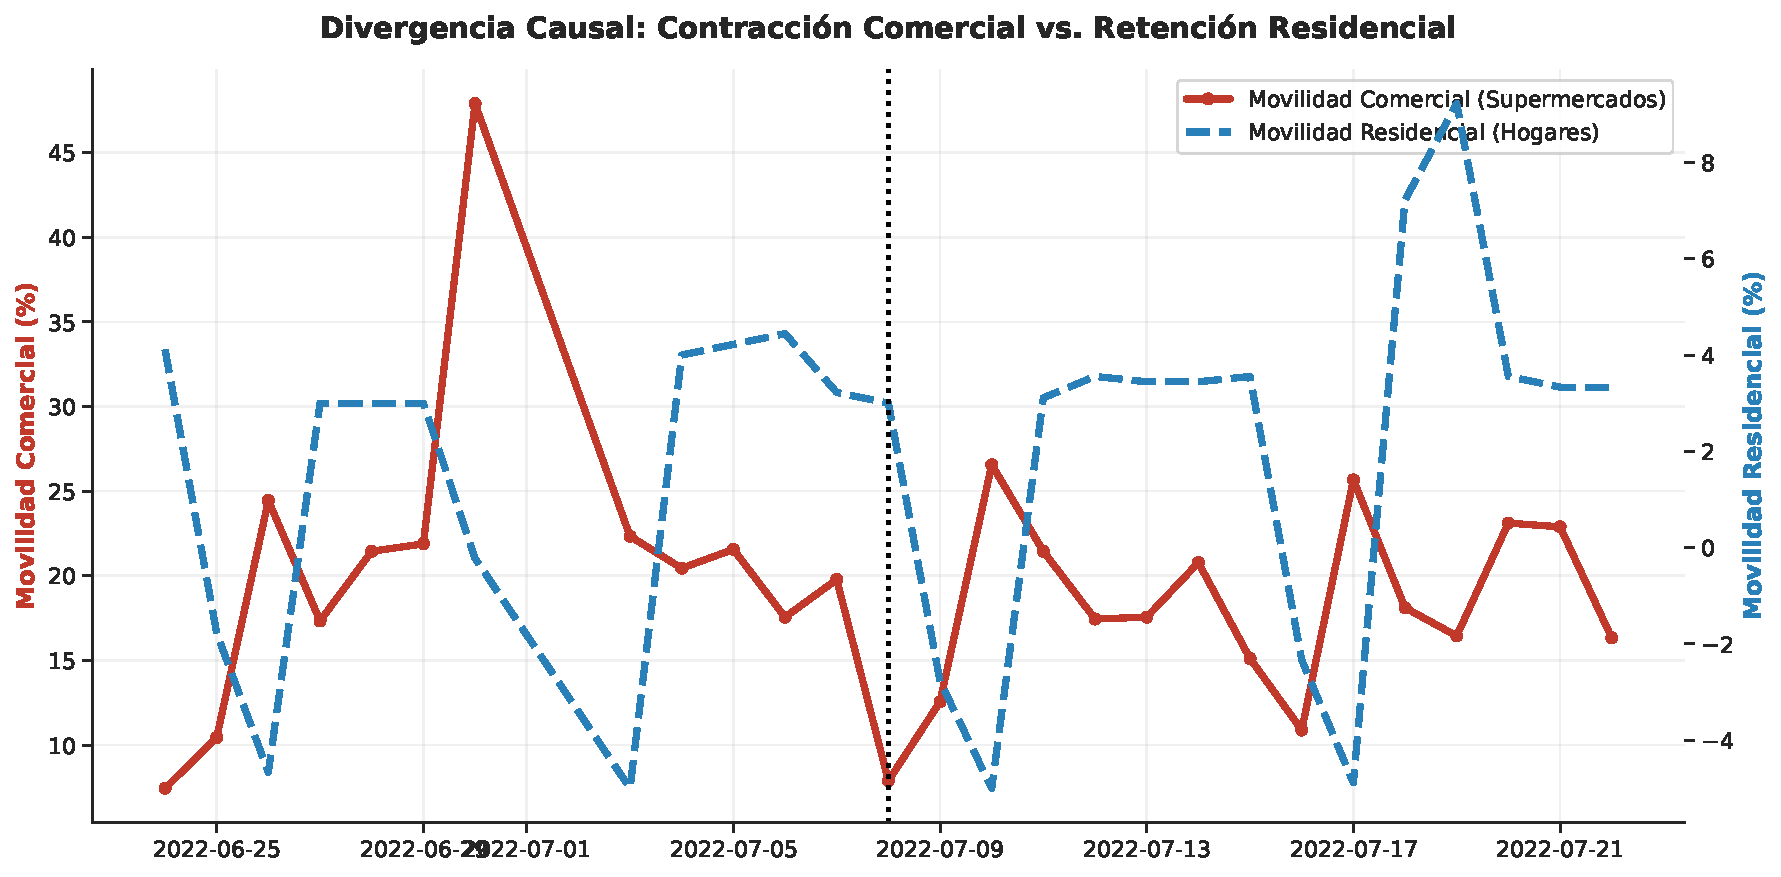
\includegraphics[width=0.85\textwidth]{figures/fig1_killer_chart.pdf}
    \caption{Hecho estilizado: Evoluci\'on de la movilidad nacional agregada en $T_0$.}
    \label{fig:killer_chart}
    \vspace{0.15cm}
    {\small Nota. El gr\'afico ilustra la contracci\'on de los flujos de movilidad f\'isica dirigida hacia sectores de consumo comercial minorista (supermercados y farmacias $Y_{it,\text{grocery}}$, l\'inea continua) en relaci\'on con el incremento simult\'aneo de la permanencia dentro de los hogares (movilidad residencial $Y_{it,\text{residential}}$, l\'inea punteada) durante el d\'ia de la interrupci\'on en la infraestructura de telecomunicaciones (l\'inea vertical correspondiente al per\'iodo cero).}
\end{figure}

\subsection{Objetivos e Hip\'otesis}
\label{sec:1_2}

Ante este escenario dentro de la econom\'ia de redes, aplicado al caso emp\'irico de Canad\'a 2022, la presente investigaci\'on estructura su an\'alisis en torno a la siguiente pregunta:

\begin{quote}
?`En qu\'e medida la exposici\'on estructural a una interrupci\'on sist\'emica en la infraestructura de telecomunicaciones determina la contracci\'on causal sobre el consumo f\'isico inel\'astico, y existe evidencia emp\'irica de que la densidad espacial de redundancia anal\'ogica (cajeros autom\'aticos) logre mitigar esta fricci\'on transaccional en una econom\'ia hiper-digitalizada?
\end{quote}

En este contexto, se plantea la siguiente Hip\'otesis de Trabajo ($H_1$): El colapso de un nodo cr\'itico en la infraestructura telem\'atica induce una contracci\'on significativa en el consumo inel\'astico que escala proporcionalmente a la exposici\'on de la red local, mientras que la densidad espacial de contingencia anal\'ogica (ATMs) exhibe una eficacia nula como mitigador macroecon\'onico debido al acoplamiento estructural entre la capa f\'isica y la capa l\'ogica del sistema de pagos.

\textbf{Objetivo General:} \\
Analizar emp\'iricamente la fricci\'on macroecon\'omica generada por fallos estoc\'asticos en la capa de infraestructura transaccional y evaluar la eficacia topol\'ogica de la redundancia anal\'ogica durante el apag\'on de Rogers (2022) en Canad\'a, utilizando un dise\~no de inferencia causal de intensidad continua.

\vspace{0.3cm}
\textbf{Objetivos Espec\'ificos:}
\begin{enumerate}
    \item Estimar el efecto causal del apag\'on tecnol\'ogico sobre la movilidad de consumo inel\'astico aislando la fricci\'on de liquidaci\'on mediante un estimador de Triple Diferencias (DDD), contrastando sectores dependientes de pagos (supermercados) frente a sectores de control (parques p\'ublicos y otros).
    \item Cuantificar la sensibilidad del impacto econ\'omico condicionada a la intensidad del tratamiento, parametrizando la exposici\'on topol\'ogica mediante la cuota de mercado provincial (\textit{Market Share}) de la red vulnerada.
    \item Testear emp\'iricamente la hip\'otesis de fallos en cascada en redes interdependientes, evaluando si el efecto base de la fricci\'on es mitigado por la densidad de infraestructura f\'isica (cajeros autom\'aticos per c\'apita).
    \item Garantizar la consistencia de la inferencia estad\'istica en un panel con agregaci\'on espacial limitada ($N=9$) mediante la implementaci\'on de un algoritmo manual de remuestreo iterativo \textit{Wild Cluster Bootstrap}, asegurando la validez interna frente al sesgo de cl\'usteres peque\~nos y la heterocedasticidad.
\end{enumerate}

\newpage
\section{Cap\'itulo II: Marco Te\'orico --- CIA vs. SIA}\label{capitulo2}

Para evaluar los canales mediante los cuales una interrupci\'on t\'ecnica en los sistemas de comunicaci\'on genera fluctuaciones en el consumo agregado, es necesario analizar la evoluci\'on conceptual del dinero en las teor\'ias de intercambio y fricciones de mercado. El argumento central de este marco te\'orico postula que los modelos macroecon\'omicos convencionales asumen restricciones de liquidez que no logran capturar las fricciones operativas y la dependencia infraestructural que caracterizan a los sistemas de pago electr\'onicos contempor\'aneos.

\subsection{La Restricci\'on Cash-in-Advance (CIA)}
\label{sec:2_1}

La teor\'ia monetaria moderna ha dedicado una extensa literatura a explicar 
por qu\'e los agentes mantienen dinero a pesar de la existencia de activos 
alternativos con mayores rendimientos financieros. Una de las respuestas m\'as 
influyentes proviene de los modelos de restricciones transaccionales, desarrollados 
inicialmente por Clower y posteriormente formalizados en modelos de equilibrio 
general din\'amico por Lucas y Stokey, donde el dinero cumple una funci\'on 
instrumental indispensable para la realizaci\'on de intercambios \citep{lucas1987money, clower1967reconsideration}.

En este enfoque, la capacidad de consumo de los hogares se encuentra limitada por 
la disponibilidad previa de saldos monetarios l\'iquidos. La denominada restricci\'on 
\textit{Cash-in-Advance} (CIA) establece que determinados bienes s\'olo pueden 
adquirirse utilizando dinero previamente acumulado, generando una fricci\'on que 
vincula directamente la demanda de dinero con el gasto corriente. Esta formulaci\'on 
permiti\'o incorporar el dinero dentro de modelos de equilibrio general sin abandonar 
la racionalidad optimizadora caracter\'istica de la tradici\'on neocl\'asica 
\citep{woodford2003interest, lucas1987money}.

Formalmente, para un hogar $i$ en el per\'iodo $t$, la restricci\'on puede expresarse como:
\begin{equation}
P_t C_{i,t} \leq m_{i,t-1} + (g_t - 1)M_{t-1}
\end{equation}
donde el valor nominal del consumo se encuentra limitado por los saldos monetarios 
heredados del per\'iodo anterior y por las transferencias monetarias derivadas de 
la expansi\'on de la oferta monetaria agregada.

A nivel agregado, la condici\'on equivalente implica que el gasto total de la 
econom\'ia debe estar respaldado por la disponibilidad de medios de pago l\'iquidos:
\begin{equation}
P(s_t)C(s_t) \leq M(s_t)
\end{equation}

La intuici\'on econ\'omica detr\'as de esta formulaci\'on es que la restricci\'on 
relevante para la actividad econ\'omica es la escasez de liquidez. En consecuencia, 
las fluctuaciones del gasto agregado emergen fundamentalmente de cambios en la 
disponibilidad de dinero o cr\'edito y no de limitaciones operativas en los 
mecanismos utilizados para transferir dichos recursos \citep{woodford2003interest, lucas1987money}.

Sin embargo, esta representaci\'on fue desarrollada en un contexto donde el acto de 
pago se conceb\'ia como una transferencia relativamente directa entre agentes. Incluso 
en formulaciones posteriores que incorporan costos de transacci\'on, innovaci\'on 
financiera y medios de pago alternativos, el supuesto impl\'icito contrinu\'a siendo 
que los saldos monetarios disponibles pueden transformarse efectivamente en pagos 
una vez que el agente decide utilizarlos \citep{lagos2005unified, alvarez2009financial, kahn2009pay}.

La creciente digitalizaci\'on de los sistemas de pago introduce una dimensi\'on 
adicional. En econom\'ias donde una proporci\'on sustancial de las transacciones 
depende de plataformas electr\'onicas, la existencia de un saldo monetario positivo 
constituye una condici\'on necesaria pero no suficiente para completar 
una operaci\'on comercial. La ejecuci\'on efectiva del pago requiere adem\'as la 
disponibilidad de infraestructura de telecomunicaciones, sistemas de autenticaci\'on, 
redes de compensaci\'on y mecanismos de autorizaci\'on operando de forma coordinada 
\citep{auer2020technology, kahn2009pay}.

Desde esta perspectiva, la literatura tradicional de restricciones monetarias describe 
adecuadamente la disponibilidad de liquidez, pero resulta menos expl\'icita respecto 
de la capacidad operativa necesaria para transformar dicha liquidez en transacciones. Esta observaci\'on motiva la introducci\'on de una extensi\'on conceptual denominada \textit{Settlement-in-Advance} (SIA), presentada en la siguiente secci\'on, cuyo objetivo es modelar la dependencia de la actividad econ\'omica respecto de la infraestructura tecnol\'ogica que sostiene los sistemas modernos de pago.

\subsection{Settlement-in-Advance (SIA): Una Extensi\'on Operacional para Econom\'ias Digitalizadas}
\label{sec:2_2}

La creciente digitalizaci\'on de los medios de pago ha modificado las condiciones 
bajo las cuales los agentes transforman saldos monetarios en transacciones 
efectivas. Mientras que los modelos monetarios tradicionales enfatizan la 
disponibilidad de liquidez como condici\'on necesaria para el intercambio 
\citep{lucas1987money, woodford2003interest}, en econom\'ias con elevada adopci\'on de pagos 
electr\'onicos la ejecuci\'on de una transacci\'on tambi\'en depende de la 
disponibilidad operativa de la infraestructura tecnol\'ogica que permite 
autenticar, transmitir y compensar \'ordenes de pago \citep{kahn2009pay, auer2020technology}.

Bajo esta perspectiva, la capacidad de gasto de los hogares no depende 
exclusivamente de la tenencia de dinero, sino tambi\'en de la posibilidad de 
convertir dicho saldo en una liquidaci\'on efectiva. La infraestructura de 
telecomunicaciones, los centros de procesamiento de datos y las plataformas de 
compensaci\'on constituyen insumos complementarios para la realizaci\'on de 
transacciones electr\'onicas. En consecuencia, interrupciones en estas capas 
pueden generar restricciones transitorias sobre el intercambio aun cuando los 
agentes mantengan posiciones de liquidez suficientes.

Esta idea puede interpretarse como una extensi\'on operacional de la restricci\'on 
\textit{Cash-in-Advance}. En lugar de asumir que los saldos monetarios son 
instant\'aneamente utilizables, el enfoque \textit{Settlement-in-Advance} 
incorpora una condici\'on adicional asociada al estado de funcionamiento de la 
infraestructura transaccional.

\begin{figure}[H]
\centering
\begin{tikzpicture}[>=Stealth, thick, font=\small]
    
    \node[draw, rectangle, rounded corners, minimum width=9cm, minimum height=1.2cm, fill=gray!10, align=center] (prod) at (0,4.2) {Capa de Producci\'on (Econom\'ia Real) \\ Acumulaci\'on de Capital, Empleo y Tecnolog\'ia Productiva};
    
    \node[draw, rectangle, rounded corners, minimum width=9cm, minimum height=1.2cm, fill=gray!20, align=center] (mon) at (0,2.1) {Capa Monetaria y Financiera \\ Oferta Monetaria, Cr\'edito y Canales de Liquidez};
    
    \node[draw, rectangle, rounded corners, minimum width=9cm, minimum height=1.2cm, fill=blue!10, align=center] (til) at (0,0) {Capa de Infraestructura Transaccional \\ Redes de Telecomunicaciones, Suministro El\'ectrico y Procesamiento de Datos};
    
    \draw[<->, line width=1.2pt] (prod) -- node[right, font=\footnotesize, xshift=0.1cm] {Demanda de Bienes y Servicios} (mon);
    \draw[<->, line width=1.2pt] (mon) -- node[right, font=\footnotesize, xshift=0.1cm, align=left] {Restricci\'on de Liquidaci\'on \\ (Fricci\'on SIA: $\Omega_t \in [0,1]$)} (til);

\end{tikzpicture}
\caption{La Arquitectura Macroecon\'omica de Tres Capas Interdependientes.}
\label{fig:til_capas}
\vspace{0.15cm}
{\small Nota.} Esquema de la cadena de dependencia en econom\'ias con sistemas de pago integrados. La materializaci\'on de las transacciones en la econom\'ia real se encuentra condicionada por la estabilidad y disponibilidad operativa de la infraestructura de comunicaciones subyacente.
\end{figure}

La Figura \ref{fig:til_capas} resume esta estructura de dependencias. La actividad econ\'omica 
observable se apoya sobre una capa monetaria y financiera cuya capacidad de 
procesamiento depende, a su vez, de una infraestructura tecnol\'ogica subyacente. 
La interrupci\'on de alguno de estos componentes puede limitar temporalmente la 
capacidad de liquidaci\'on del sistema de pagos y reducir el volumen de 
transacciones realizadas.

Para formalizar esta idea, se introduce un par\'ametro de disponibilidad operativa, 
$\Omega_t \in [0,1]$, que captura el grado de funcionamiento de la infraestructura 
transaccional en cada per\'iodo. A nivel microecon\'omico, la capacidad de consumo 
de un hogar puede representarse mediante la siguiente restricci\'on:
\begin{equation}
P_t C_{i,t} \leq V_c m^c_{i,t} + \Omega_t V_d m^d_{i,t}
\end{equation}
donde $m^c_{i,t}$ representa los saldos mantenidos en efectivo y $m^d_{i,t}$ los 
saldos digitales. Los par\'ametros $V_c$ y $V_d$ reflejan la eficiencia transaccional 
relativa de cada instrumento de pago. En condiciones eficientes, los medios digitales 
suelen presentar menores costos de transacci\'on y mayor velocidad de procesamiento 
que el efectivo \citep{lagos2005unified, alvarez2009financial}.

A nivel agregado, la restricci\'on puede expresarse como:
\begin{equation}
P(s_t)C(s_t) \leq V_c M_c(s_t) + \Omega_t(s_t)V_d M_d(s_t)
\end{equation}
donde $M_c$ y $M_d$ representan los agregados monetarios f\'isicos y digitales de 
la econom\'ia.

La interpretaci\'on econ\'omica de esta especificaci\'on difiere de la restricci\'on 
CIA convencional. En este caso, la limitaci\'on sobre el gasto no surge necesariamente 
de una insuficiencia de saldos monetarios, sino de una reducci\'on en la capacidad 
de procesamiento y liquidaci\'on del sistema de pagos. Cuando $\Omega_t$ disminuye 
debido a una interrupci\'on tecnol\'ogica, la capacidad efectiva de utilizar medios 
digitales se contrae aun cuando los balances de los agentes permanezcan inalterados.

Este mecanismo resulta consistente con la literatura sobre interdependencia de 
redes e infraestructuras cr\'iticas, que muestra c\'omo perturbaciones localizadas 
pueden propagarse entre sistemas funcionalmente conectados \citep{buldyrev2010catastrophic, battiston2012liaisons, acemoglu2012network}. En particular, la infraestructura de pagos puede 
interpretarse como una red interdependiente en la que la capa financiera depende 
de la continuidad operativa de las redes de comunicaci\'on y procesamiento de datos.

Asimismo, la literatura reciente sobre adopci\'on tecnol\'ogica sugiere que una mayor 
utilizaci\'on de medios de pago electr\'onicos incrementa la eficiencia transaccional 
en condiciones normales, pero tambi\'en puede aumentar la exposici\'on agregada 
frente a interrupciones de infraestructura cuando existen pocas alternativas de 
sustituci\'on inmediata \citep{crouzet2023shocks}. En este contexto, el efectivo conserva 
un papel residual como mecanismo de contingencia capaz de sostener una fracci\'on 
de las transacciones cuando los canales digitales se encuentran temporalmente 
afectados \citep{alvarez2009financial}.

Finalmente, la relaci\'on entre infraestructura digital y actividad econ\'omica 
puede entenderse mediante el concepto de redes multicapa o \textit{multiplex}. 
En estas estructuras, los mismos agentes participan simult\'aneamente en distintas 
capas funcionales ---comunicaciones, pagos y mercados de bienes--- de modo que una 
interrupci\'on en una de ellas puede afectar el funcionamiento de las restantes 
\citep{dedomenico2013mathematical, kivela2014multilayer}. Desde esta perspectiva, el par\'ametro $\Omega_t$ resume el grado de operatividad de la infraestructura transaccional y constituye el principal canal mediante el cual una falla tecnol\'ogica puede trasladarse hacia variables econ\'omicas agregadas. Para profundizar en el marco matemático mirar Anexo \ref{anx:anexo_b}.

\subsection{La Capa de Infraestructura Transaccional y Canales de Transmisi\'on}
\label{sec:2_3}

La ejecuci\'on de pagos electr\'onicos depende del funcionamiento coordinado de 
m\'ultiples componentes tecnol\'ogicos interdependientes. A diferencia de los 
modelos monetarios tradicionales, donde el intercambio se representa como una 
operaci\'on bilateral entre agentes, las econom\'ias digitalizadas requieren una 
infraestructura compleja compuesta por redes de telecomunicaciones, sistemas de 
procesamiento de datos, plataformas de compensaci\'on financiera y mecanismos de 
respaldo operativo \citep{kahn2009pay, auer2020technology}.

Desde la perspectiva de la teor\'ia de redes, estos elementos pueden interpretarse 
como capas complementarias de una arquitectura econ\'omica integrada. La literatura 
sobre redes complejas muestra que sistemas altamente conectados suelen exhibir 
ganancias importantes de eficiencia, aunque tambi\'en pueden amplificar 
perturbaciones cuando existen dependencias cr\'iticas entre nodos o sectores 
\citep{acemoglu2012network, battiston2012liaisons, elliott2014financial, golub20222fragilitysurvey}.

Con el fin de representar esta dependencia tecnol\'ogica, la capacidad agregada 
de procesamiento transaccional puede modelarse mediante una funci\'on de 
disponibilidad infraestructural:
\begin{equation}
N_t = G(E_t, T_t, C_t, B_t, A_t)
\end{equation}
donde:
\begin{itemize}
    \item $E_t$ representa la continuidad del suministro el\'ectrico;
    \item $T_t$ el estado operativo de las redes de telecomunicaciones;
    \item $C_t$ la capacidad de procesamiento computacional;
    \item $B_t$ la disponibilidad de la infraestructura bancaria y de compensaci\'on;
    \item $A_t$ la capacidad operativa de los mecanismos alternativos de liquidaci\'on.
\end{itemize}

Bajo esta formulaci\'on, los distintos componentes operan como insumos 
complementarios. La reducci\'on significativa de cualquiera de ellos puede 
restringir la capacidad total de procesamiento del sistema, incluso cuando el 
resto de los componentes permanezcan operativos. Esta l\'ogica es consistente con 
los modelos de redes interdependientes desarrollados por \cite{buldyrev2010catastrophic} y con la literatura sobre vulnerabilidad sist\'emica en estructuras multicapa 
\citep{dedomenico2013mathematical, kivela2014multilayer}.

\begin{figure}[H]
\centering
\vspace{0.3cm}
\begin{tikzpicture}[
    >=Stealth, 
    thick, 
    font=\small,
    node distance=0.8cm,
    box/.style={draw, rectangle, rounded corners, text width=3.3cm, align=center, minimum height=1.5cm}
]
    
    \node[box, fill=gray!10] (infra) {Infraestructura F\'isica \\ (Fallas T\'ecnicas, Errores de Configuraci\'on)};
    
    \node[box, fill=gray!15, right=of infra] (estado) {Disrupci\'on de Red \\ shock L\'ogica TIL: \\ ($\Omega_t = 0$)};
    
    \node[box, fill=blue!10, right=of estado] (gamma) {Intensidad de Exposici\'on \\ Cuota de Mercado: \\ ($\text{Exposure}_i$)};
    
    \node[box, fill=red!10, right=of gamma] (vol) {Impacto Agregado \\ Par\'alisis Comercial y Volatilidad ($Y_{i,t}$)};
    
    % Flujo causal secuencial horizontal (Corregido: ya no está cortado)
    \draw[->, line width=1.1pt] (infra) -- (estado);
    \draw[->, line width=1.1pt] (estado) -- (gamma);
    \draw[->, line width=1.1pt] (gamma) -- (vol);
    
    % Mecanismos superiores analíticos
    \draw[->, line width=1.1pt] (estado.north) to[bend left=30] 
        node[above, yshift=0.1cm, font=\footnotesize] {Fricci\'on Transaccional SIA} (gamma.north);
        
    \draw[->, line width=1.1pt] (gamma.north) to[bend left=30] 
        node[above, yshift=0.1cm, font=\footnotesize] {Efectos de Desborde Espacial} (vol.north);
        
    % Canal de transmisión directa (Canal macro-logístico horizontal)
    \draw[->, dashed, line width=1pt] (estado.south) to[bend right=25] 
        node[below, align=center, yshift=-0.15cm, font=\footnotesize] {Canal de Transmisi\'on Directo de Infraestructura} (vol.south);
        
\end{tikzpicture}
\vspace{0.3cm}
\caption{Mecanismo Estructural de Transmisi\'on del shock Tecnol\'ogico.}
\label{fig:causal_flow_expanded}
\vspace{0.15cm}
{\small Nota.} Diagrama de propagaci\'on del riesgo de infraestructura. Una falla en la capa l\'ogica detona la interrupci\'on del servicio ($\Omega_t = 0$). La magnitud del impacto sobre el vaciado de los mercados y las din\'amicas log\'isticas agregadas est\'a condicionada por el grado previo de exposici\'on digital ($\text{Exposure}_i$) de los agentes en cada econom\'ia regional.
\end{figure}

La Figura \ref{fig:causal_flow_expanded} resume el mecanismo conceptual de transmisi\'on considerado en este trabajo. Un \textit{shock} originado en la infraestructura f\'isica o l\'ogica de comunicaciones afecta inicialmente la capacidad de procesamiento de la red de 
pagos. La magnitud de dicho impacto depende del grado de exposici\'on previa de 
los agentes econ\'omicos a la infraestructura afectada. A medida que la 
interrupci\'on reduce la disponibilidad de los canales de liquidaci\'on, emerge 
la fricci\'on \textit{Settlement-in-Advance} descrita en la secci\'on anterior, 
restringiendo temporalmente la capacidad de realizar transacciones.

La literatura reciente sobre propagaci\'on de \textit{shocks} enfatiza que la 
importancia de una perturbaci\'on no depende \'unicamente de su tama\~no inicial, 
sino tambi\'en de la posici\'on estructural del nodo afectado dentro de la red. 
Cuando una falla ocurre en un nodo altamente central, sus efectos pueden extenderse 
m\'as all\'a de la regi\'on o sector donde se origina, generando consecuencias 
agregadas desproporcionadas respecto del \textit{shock} inicial 
\citep{acemoglu2012network, carvalho2014micro}.

\begin{figure}[H]
    \centering
    \includegraphics[width=0.85\textwidth]{figures/fig4_gradiente.pdf}
    \caption{Gradiente te\'orico de exposici\'on estructural ante fallas de infraestructura.}
    \label{fig:gradiente_exposicion}
    \vspace{0.15cm}
    {\small Nota.} Representaci\'on esquem\'atica de la vulnerabilidad intercapas, que ilustra c\'omo la densidad poblacional y la tasa de adopci\'on transaccional digital determinan la pendiente del impacto econ\'omico potencial ante una falla en los nodos centrales de comunicaci\'on.
\end{figure}

La Figura \ref{fig:gradiente_exposicion} ilustra esta idea mediante un gradiente te\'orico de exposici\'on estructural. Las econom\'ias regionales no presentan el mismo grado de dependencia respecto de una determinada infraestructura de comunicaciones o 
proveedor de servicios. Como consecuencia, una interrupci\'on tecnol\'ogica 
com\'un puede generar respuestas heterog\'eneas en funci\'on del nivel de 
adopci\'on de medios digitales, la concentraci\'on de mercado de los proveedores 
afectados y la existencia de mecanismos alternativos de liquidaci\'on.

Este mecanismo resulta particularmente relevante en sistemas donde la actividad 
econ\'omica depende crecientemente de plataformas digitales de pago. Diversos 
estudios muestran que la adopci\'on de tecnolog\'ias financieras mejora la 
eficiencia transaccional y reduce costos de intercambio, pero tambi\'en 
incrementa la dependencia de infraestructuras especializadas cuyo funcionamiento 
se vuelve cr\'itico para la coordinaci\'on econ\'omica cotidiana 
\citep{jack2014risk, auer2020technology, crouzet2023shocks}.

\begin{figure}[H]
\centering
\resizebox{0.92\textwidth}{!}{
\begin{tikzpicture}[node distance=0.5cm and 1.5cm, auto,
    block/.style={rectangle, draw, fill=gray!10, text width=13em, align=center, rounded corners, minimum height=3em},
    line/.style={draw, -{Stealth}, thick}]
    
    \node [block] (shock) {Shock de Infraestructura \\ (Fallo BGP en $T=0$)};
    \node [block, below=of shock] (payments) {Disrupci\'on Multiplex \\ (Colapso del Canal de Pagos)};
    \node [block, below=of payments] (frictions) {Restricci\'on SIA \\ (Fricci\'on de Liquidaci\'on Agregada)};
    \node [block, below=of frictions] (delay) {Fase $A_{\text{R}}$: Par\'alisis \\ (Contracci\'on de Movilidad Esencial)};
    \node [block, below=of delay] (catchup) {Fase $A_{\text{C}}$: Compensaci\'on \\ (Reacomodamiento en $T+2$)};
    
    \node [block, right=of payments] (atm) {Resiliencia Anal\'ogica \\ $\partial\text{Shock}/\partial\text{ATM} \approx 0$ \\ (Fallo en Cascadas Acoplado)};
    \node [block, left=of delay] (hub) {Centralidad Asim\'etrica \\ $s_{i} \gg s_j$ \\ (Origen del Impulso Agregado)};

    \path [line] (shock) -- (payments);
    \path [line] (payments) -- (frictions);
    \path [line] (frictions) -- (delay);
    \path [line] (delay) -- (catchup);
    
    \path [line, dashed] (payments) -- (atm);
    \path [line, dashed] (hub) -- (delay);
    
\end{tikzpicture}}
\caption{Diagrama de Flujo Conceptual: Canal de Transmisi\'on del Marco SIA/TIL.}
\label{fig:diagrama_conceptual_es}
\end{figure}

La Figura \ref{fig:diagrama_conceptual_es} esquematiza la transmisi\'on din\'amica y secuencial del \textit{shock} infraestructural bajo el marco unificado SIA/TIL. El desencadenante tecnol\'ogico (fallo BGP en $T=0$) provoca una disrupci\'on \textit{multiplex} instant\'anea que paraliza el canal digital de validaci\'on de transacciones. Esta perturbaci\'on activa la restricci\'on \textit{Settlement-in-Advance} (SIA) a nivel agregado, transform\'andose en una fricci\'on de liquidaci\'on que restringe de forma asim\'etrica el vaciado de los mercados regionales seg\'un su centralidad ($s_i \gg s_j$). El sistema experimenta entonces dos etapas temporales diferenciadas: una fase de par\'alisis contempor\'anea ($A_{R}$), caracterizada por la contracci\'on severa de la movilidad esencial, y una fase posterior de compensaci\'on log\'istica ($A_{C}$) en $T+2$. El diagrama evidencia que la densidad f\'isica alternativa
\begin{equation}
\frac{\partial \text{Shock}}{\partial \text{ATM}} \approx 0
\end{equation}
es incapaz de romper el acoplamiento estructural intercapas, consolidando un fallo en cascada que propaga la vulnerabilidad l\'ogica hacia la actividad comercial de la econom\'ia real.. Para profundizar en el marco matemático ver \nobreak{Anexo \ref{anx:anexo_b}}.

\subsection{Marco Institucional}

El episodio analizado en esta investigaci\'on corresponde a la interrupci\'on 
masiva de servicios ocurrida en Canad\'a el 8 de julio de 2022. La falla se 
origin\'o durante una actualizaci\'on programada de la infraestructura de red de 
Rogers Communications, uno de los principales proveedores de telecomunicaciones 
del pa\'is. De acuerdo con la investigaci\'on oficial posterior, un error de 
configuraci\'on afect\'o el funcionamiento del protocolo \textit{Border Gateway 
Protocol} (BGP), generando la desconexi\'on de la red AS812 del resto de 
Internet y provocando una interrupci\'on nacional de los servicios de 
conectividad \citep{crtc2024rogers, rogers2022q3}.

Desde la perspectiva de identificaci\'on emp\'irica, este episodio resulta 
particularmente relevante porque constituye una perturbaci\'on tecnol\'ogica 
ex\'ogena respecto de las condiciones econ\'omicas regionales. La interrupci\'on 
no estuvo asociada a cambios en ingresos, precios, empleo o pol\'itica 
econ\'omica, sino a un fallo operativo inesperado en una infraestructura 
cr\'itica de comunicaciones.

\begin{figure}[H]
    \centering
    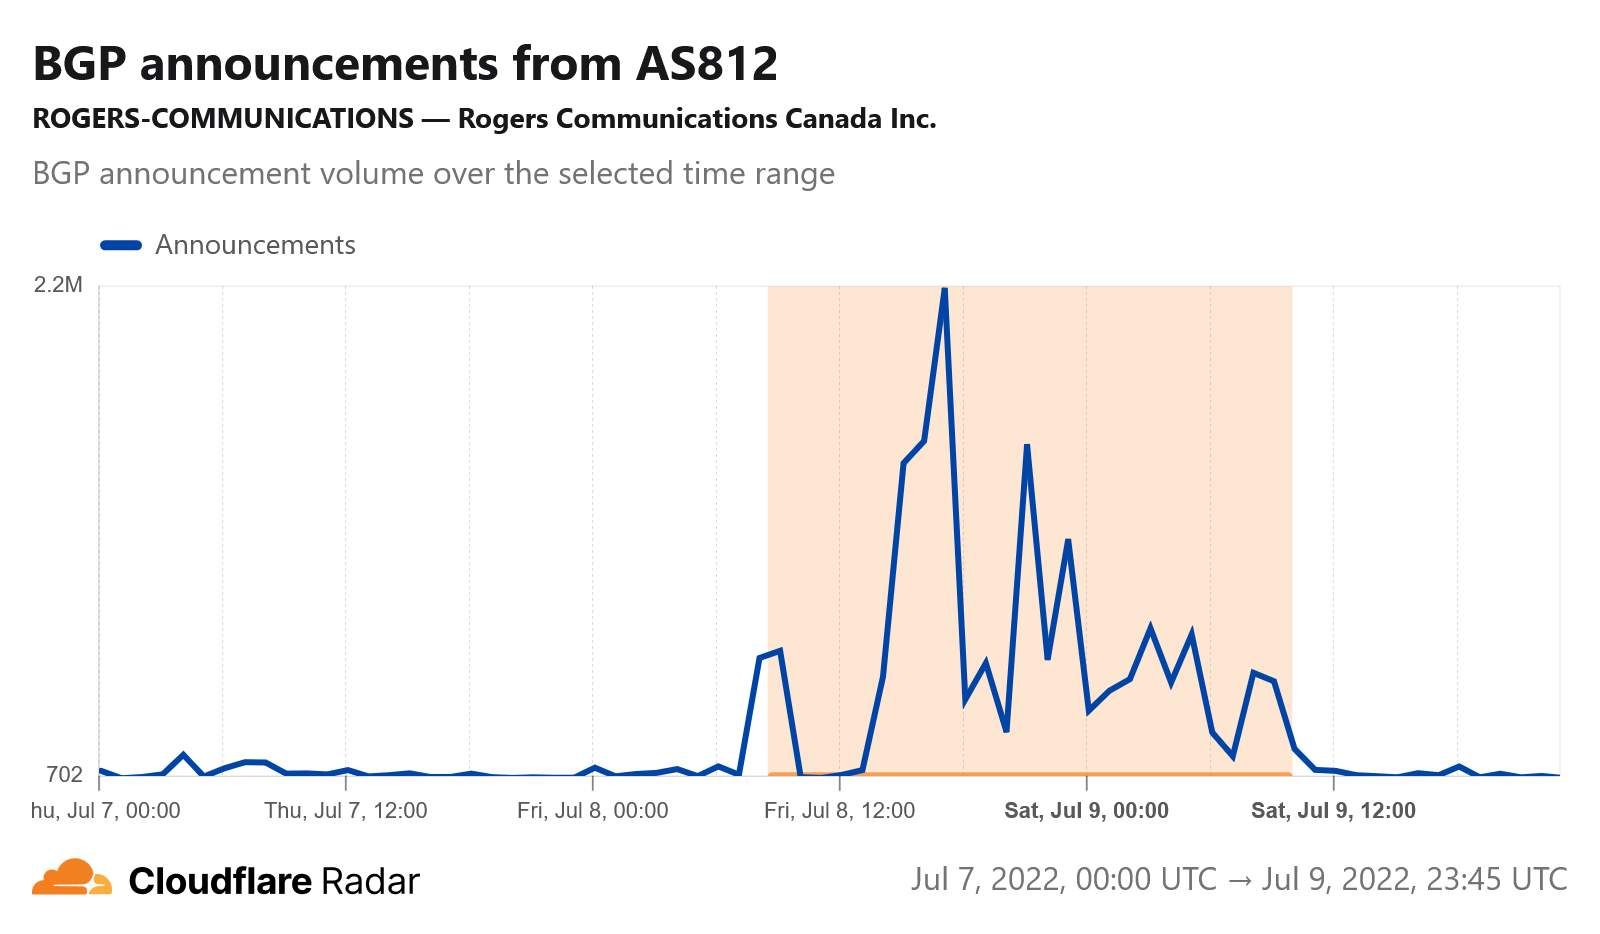
\includegraphics[width=0.85\textwidth]{figures/cloudflare-radar_bgp-announcements-xy_as812_20220707-20220709.png}
    \caption{Volatilidad en la capa de transporte de red: Anuncios BGP del AS812 (Rogers).}
    \label{fig:cloud_bgp}
    \vspace{0.15cm}
    {\small Nota. Registros de Cloudflare Radar correspondientes al volumen de anuncios BGP (Border Gateway Protocol) del Sistema Aut\'onomo AS812. El incremento an\'omalo de anuncios refleja la inestabilidad en el enrutamiento l\'ogico de la red entre el 7 y el 9 de julio de 2022.}
\end{figure}

La Figura \ref{fig:cloud_bgp} presenta la evoluci\'on de los anuncios BGP correspondientes al sistema aut\'onomo AS812 de Rogers. Los registros muestran una alteraci\'on abrupta en la din\'amica normal de enrutamiento durante el per\'iodo del 
incidente. La anomal\'ia observada refleja la p\'erdida de estabilidad de las rutas necesarias para intercambiar tr\'afico con otras redes, constituyendo la manifestaci\'on t\'ecnica inicial del \textit{shock} \citep{crtc2024rogers}.

La interrupci\'on del sistema de enrutamiento tuvo consecuencias inmediatas sobre 
la capacidad de transmisi\'on de datos de la red afectada.

\begin{figure}[H]
    \centering
    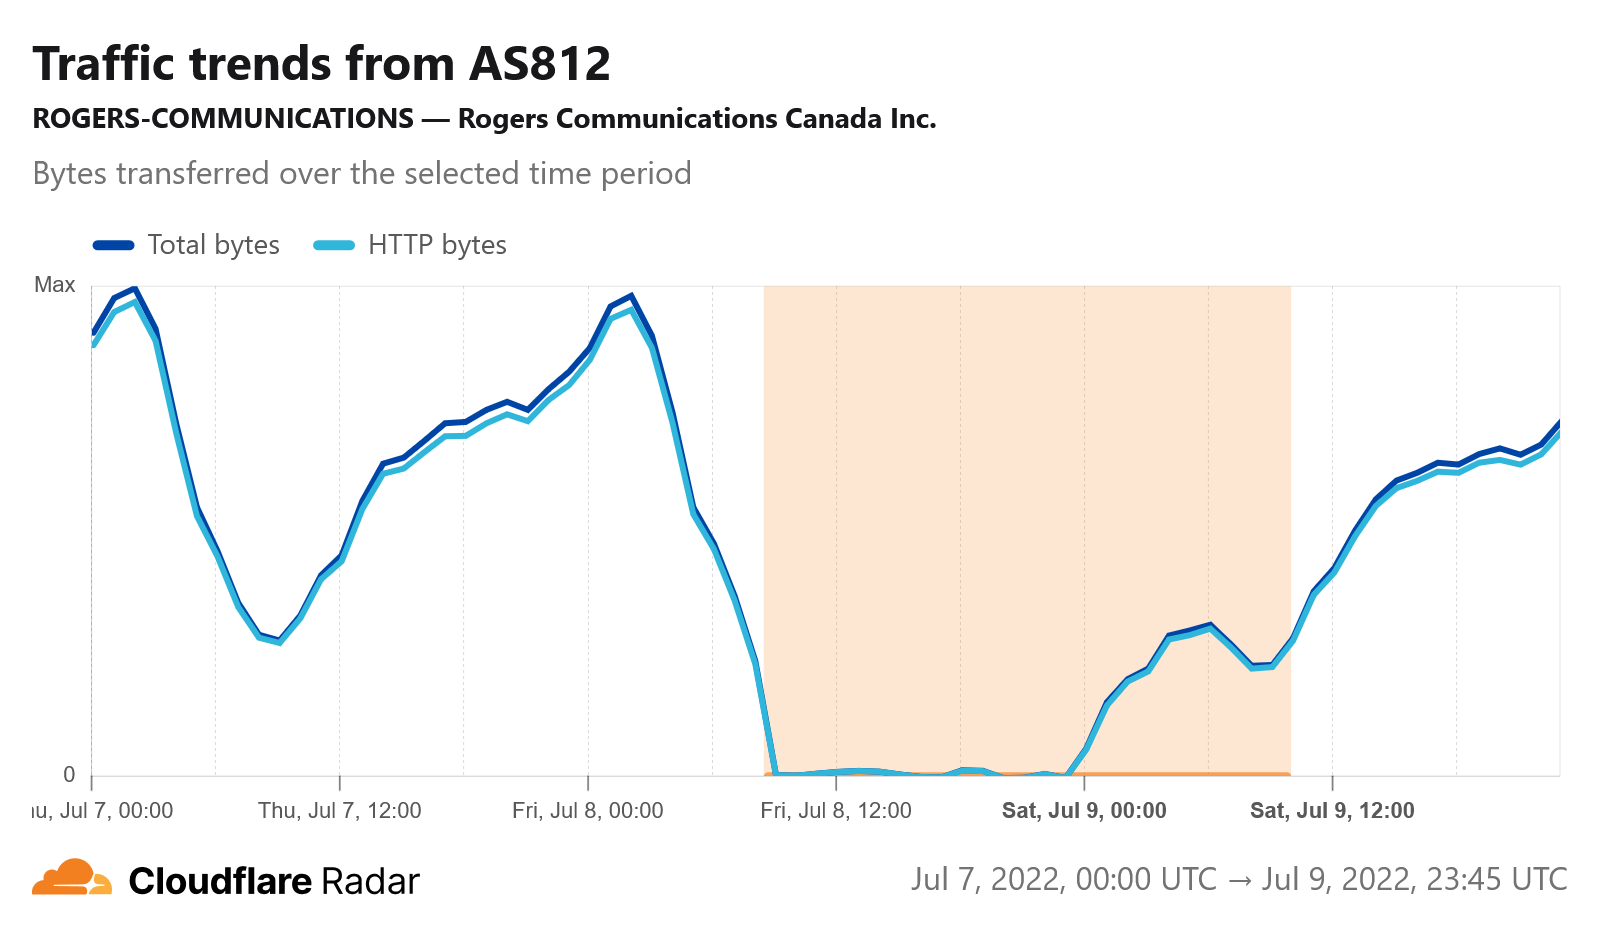
\includegraphics[width=0.85\textwidth]{figures/cloudflare-radar_traffic-trends-xy_as812_20220707-20220709.png}
    \caption{Consecuencia operativa del fallo: Tr\'afico HTTP y datos del AS812.}
    \label{fig:cloud_traffic}
    \vspace{0.15cm}
    {\small Nota. Evoluci\'on temporal del tr\'afico de datos de la red afectada. Se observa la contracci\'on del flujo digital a partir de las primeras horas del viernes 8 de julio de 2022, operando como un shock tecnol\'ogico ex\'ogeno de car\'acter transitorio.}
\end{figure}

La Figura \ref{fig:cloud_traffic} muestra la evoluci\'on del tr\'afico HTTP asociado a la 
infraestructura de Rogers. Luego del evento de configuraci\'on, el volumen de tr\'afico experiment\'o una ca\'ida abrupta respecto de sus niveles habituales, evidenciando una p\'erdida sustancial de conectividad. Desde la perspectiva del marco SIA desarrollado en las secciones anteriores, esta disrupci\'on puede interpretarse como una reducci\'on ex\'ogena del par\'ametro de disponibilidad operativa de la infraestructura transaccional ($\Omega_t$).

La relevancia econ\'omica de este episodio radica en que una parte importante de 
los sistemas de pagos minoristas canadienses depend\'ia directa o indirectamente 
de dicha infraestructura. En particular, la interrupci\'on afect\'o la capacidad 
operativa de la red Interac, responsable del procesamiento de pagos con tarjeta 
de d\'ebito y transferencias electr\'onicas ampliamente utilizadas por hogares y 
comercios \citep{interac2022statement}. Como consecuencia, numerosos establecimientos 
enfrentaron dificultades para validar transacciones electr\'onicas aun cuando los 
consumidores mantuvieran fondos suficientes en sus cuentas bancarias.

La estructura del mercado canadiense proporciona adem\'as una fuente de 
variaci\'on regional \'util para el an\'alisis emp\'irico. La participaci\'on de 
mercado de Rogers difer\'ia considerablemente entre provincias, generando 
distintos grados de exposici\'on potencial al \textit{shock}. Esta 
heterogeneidad permite evaluar si las regiones m\'as dependientes de la 
infraestructura afectada experimentaron mayores disrupciones econ\'omicas 
durante el evento.

\begin{figure}[H]
    \centering
    \includegraphics[width=0.85\textwidth]{figures/fig6_ontario_quebec.pdf}
    \caption{Series de movilidad observada: Ontario vs. Quebec (Pre-Shock).}
    \label{fig:ontario_quebec_raw}
    \vspace{0.15cm}
    {\small Nota. Evoluci\'on diaria de la variable dependiente de movilidad a nivel provincial. El gr\'afico ilustra que las diferencias en los niveles absolutos de actividad regional se mantienen estables, exhibiendo tendencias sincronizadas en las semanas previas al shock tecnol\'ogico.}
\end{figure}

La Figura \ref{fig:ontario_quebec_raw} presenta evidencia descriptiva para Ontario y Quebec, dos provincias con niveles sustancialmente diferentes de exposici\'on a Rogers. Ontario registraba una mayor participaci\'on de mercado del proveedor y concentraba 
adem\'as componentes cr\'iticos de la infraestructura financiera nacional. Quebec, 
en cambio, exhib\'ia una menor dependencia relativa debido a la presencia de 
operadores alternativos como Videotron y Bell.

Las series muestran una evoluci\'on relativamente paralela de la movilidad en las 
semanas previas a la interrupci\'on, lo que constituye evidencia preliminar 
consistente con el supuesto de tendencias paralelas que posteriormente ser\'a 
evaluado formalmente mediante metodolog\'ias de diferencias en diferencias 
\citep{angrist2009mostly, cunningham2021causal, callaway2021difference}. Tras la ocurrencia del \textit{shock}, Ontario exhibe una contracci\'on m\'as pronunciada de la 
actividad relativa a Quebec, en l\'inea con la hip\'otesis de que una mayor 
exposici\'on a la infraestructura afectada amplifica las consecuencias econ\'omicas 
de la interrupci\'on.

En conjunto, la evidencia institucional y descriptiva sugiere que la falla de 
Rogers constituye un experimento cuasi-natural particularmente adecuado para 
estudiar c\'omo una perturbaci\'on tecnol\'ogica en la infraestructura de 
comunicaciones puede transmitirse hacia variables econ\'omicas observables a 
trav\'es de los sistemas de pago digitales. La combinaci\'on de exogeneidad 
temporal, alcance nacional y heterogeneidad regional en la exposici\'on 
proporciona condiciones favorables para identificar emp\'iricamente los 
mecanismos propuestos por el marco \textit{Settlement-in-Advance}.

\newpage
\section{Cap\'itulo III: Datos}
\subsection{Naturaleza de los Datos}

La evaluaci\'on emp\'irica del impacto econ\'omico de la interrupci\'on de la 
red de Rogers requiere aproximar la evoluci\'on de la actividad comercial 
mediante indicadores alternativos, dado que no existen registros p\'ublicos de 
acceso abierto sobre transacciones minoristas desagregadas a nivel provincial y 
con frecuencia diaria. Siguiendo la literatura reciente que utiliza datos de 
alta frecuencia para analizar la respuesta econ\'omica ante \textit{shocks} 
ex\'ogenos, esta investigaci\'on emplea indicadores de movilidad geogr\'afica 
como variables \textit{proxy} del consumo presencial de bienes y servicios 
\citep{chetty2020economic, bounie2020consumers, stephens2014hands}.

Con este prop\'osito se construy\'o un panel balanceado de frecuencia diaria 
para nueve provincias canadienses durante el per\'iodo 2020--2022. La base de 
datos integra informaci\'on proveniente de tres fuentes principales: 
indicadores de movilidad, medidas de exposici\'on al \textit{shock} de 
telecomunicaciones y variables asociadas a la disponibilidad de infraestructura 
f\'isica de acceso al efectivo.

\begin{enumerate}
    \item \textbf{Movilidad F\'isica Agregada:} Las series de movilidad provienen de los \textit{Google COVID-19 Community 
Mobility Reports} para Canad\'a correspondientes a los a\~nos 2020, 2021 y 2022. La variable dependiente principal utilizada en esta investigaci\'on corresponde 
a la movilidad hacia supermercados, mercados de alimentos y farmacias 
(\textit{grocery and pharmacy mobility}), denotada como $Y_{i,t}^{grocery}$. Esta 
categor\'ia se considera una aproximaci\'on razonable de la demanda presencial 
de bienes esenciales y ha sido utilizada en investigaciones previas para estudiar 
el comportamiento del consumo ante perturbaciones econ\'omicas y restricciones 
operativas \citep{chetty2020economic, bounie2020consumers}.
Adicionalmente, se incorporan tres categor\'ias de movilidad para realizar 
pruebas de robustez y falsificaci\'on: movilidad hacia parques 
($Y_{i,t}^{parks}$), movilidad hacia estaciones y terminales de transporte 
($Y_{i,t}^{transit}$) y permanencia en \'areas residenciales 
($Y_{i,t}^{residential}$). Estas variables permiten evaluar si los efectos 
observados se concentran espec\'ificamente en actividades asociadas al comercio 
minorista o reflejan cambios m\'as generales en los patrones de desplazamiento 
de la poblaci\'on.
    \item \textbf{Intensidad de Exposici\'on al Shock:} La interrupci\'on de la red de Rogers no afect\'o de manera homog\'enea a todas 
las provincias canadienses. La magnitud potencial del \textit{shock} dependi\'o 
de la participaci\'on de mercado que la empresa manten\'ia en cada jurisdicci\'on 
al momento del evento.
Para capturar esta heterogeneidad se construy\'o una medida provincial de 
exposici\'on ($S_i$) utilizando la cuota de mercado de Rogers Communications 
Inc. en 2022. La informaci\'on fue obtenida a partir de los informes 
corporativos de la firma previos a la adquisici\'on de Shaw Communications 
\citep{rogers2022q3} y complementada con antecedentes regulatorios publicados por 
la \citep{crtc2024rogers}.
Esta variable funciona como una medida continua de intensidad del tratamiento. 
Provincias con una mayor presencia de Rogers enfrentaban una probabilidad 
superior de sufrir interrupciones en los servicios de conectividad y en los 
canales de pago dependientes de dicha infraestructura. En consecuencia, la 
variaci\'on geogr\'afica de estas participaciones permite identificar 
diferencias en la exposici\'on potencial al \textit{shock} tecnol\'ogico.
    \item \textbf{Disponibilidad de infraestructura de efectivo:} Con el objetivo de analizar la capacidad de sustituci\'on entre pagos digitales 
y efectivo f\'isico durante la interrupci\'on, se construy\'o una medida 
provincial de disponibilidad de cajeros autom\'aticos (ATM).
La localizaci\'on de las terminales fue obtenida mediante consultas a la base 
de datos abierta de \textit{OpenStreetMap} utilizando la plataforma 
\textit{Overpass Turbo}. Posteriormente, se contabiliz\'o el n\'umero de cajeros 
autom\'aticos existentes en cada provincia y se normaliz\'o utilizando la 
poblaci\'on provincial proveniente del Censo de Canad\'a de 2021 
\citep{statscan2021pop} obteni\'endose una medida de densidad expresada en cajeros 
por mill\'on de habitantes.
Esta variable ($A_i$) busca aproximar la disponibilidad potencial de mecanismos 
alternativos de acceso al efectivo durante episodios de interrupci\'on de los 
sistemas electr\'onicos de pago. Su construcci\'on resulta consistente con los 
criterios de cobertura geogr\'afica y acceso al efectivo analizados por el  \cite{bankofcanada2023cash}.
\end{enumerate}

El procesamiento de datos, la construcci\'on de variables y las estimaciones 
econom\'etricas se realizaron utilizando Python (versi\'on 3.10+) en un entorno 
reproducible de Google Colab. Asimismo, los ponderadores demogr\'aficos 
utilizados posteriormente en las estimaciones por m\'inimos cuadrados ponderados 
se calibraron utilizando las poblaciones provinciales reportadas por 
\cite{statscan2021pop}.

El Cuadro \ref{tab:descriptivas} presenta las estad\'isticas descriptivas de las principales variables empleadas en el an\'alisis. Para la estrategia emp\'irica se adopta 
una ventana temporal sim\'etrica de catorce d\'ias previos y catorce d\'ias 
posteriores al evento del 8 de julio de 2022 ($T=29$ d\'ias). En estudios de 
eventos de alta frecuencia, este criterio permite aislar con mayor precisi\'on 
los efectos asociados al \textit{shock} analizado y reducir la influencia de 
perturbaciones macroecon\'omicas concurrentes \citep{schmidheiny2019event, 
cunningham2021causal}.


\begin{table}[H]
    \centering
    \caption{Estad\'isticas Descriptivas del Panel de Alta Frecuencia (Ventana de $\pm$14 d\'ias)}
    \label{tab:descriptivas}
    \small
    \begin{tabular}{lccccc}
        \toprule
        M\'etrica Estad\'istica & $Y_{\text{grocery}}$ & $Y_{\text{residential}}$ & $Y_{\text{parks}}$ & $S_i$ & $A_i$ \\
        \midrule
        Observaciones Totales & 1593 & 1593 & 1456 & 1593 & 1593 \\
        Media Muestral        & 12.731   & 4.260    & 164.327  & 0.303    & 93.844   \\
        Desviaci\'on Est\'andar & 12.335   & 5.158    & 72.782   & 0.095    & 20.303   \\
        Valor M\'inimo        & -42  & -11  & -25  & 0.175    & 67.143   \\
        Valor M\'aximo        & 94   & 21   & 500  & 0.475    & 135.962  \\
        \bottomrule
    \end{tabular}
    \vspace{0.15cm}
    \begin{flushleft}
    \small{Nota. Los datos presentados corresponden a un panel de datos balanceado para las variables de movilidad ($Y$), intensidad de exposici\'on ($S_i$) y densidad de cajeros autom\'aticos ($A_i$). El s\'imbolo $\pm$ representa el entorno temporal de la ventana analizada.}
    \end{flushleft}
\end{table}


\subsection{Limitaciones de la Alta Frecuencia en Econom\'ia P\'ublica}
\label{sec:3_2}

El dise\~no emp\'irico utilizado en esta investigaci\'on presenta una serie de 
limitaciones que deben considerarse al interpretar los resultados.

En primer lugar, la variable dependiente utilizada no mide directamente el gasto 
de los hogares, sino patrones de movilidad asociados a actividades de consumo. 
La utilizaci\'on de indicadores de desplazamiento hacia supermercados, mercados 
y farmacias constituye una aproximaci\'on indirecta de la actividad transaccional, 
consistente con trabajos recientes que emplean datos de movilidad como 
indicadores de comportamiento econ\'omico de alta frecuencia \citep{chetty2020economic, 
bounie2020consumers}. Sin embargo, cambios en la movilidad no necesariamente implican 
variaciones proporcionales en el valor monetario de las transacciones realizadas. 
Por esta raz\'on, los resultados deben interpretarse como evidencia sobre 
alteraciones en la actividad comercial observable m\'as que como estimaciones 
directas de p\'erdidas de consumo.

En segundo lugar, el an\'alisis se realiza sobre un n\'umero reducido de unidades 
geogr\'aficas. La muestra comprende \'unicamente nueve provincias canadienses, lo 
que limita la validez de las aproximaciones asint\'oticas convencionales 
utilizadas en la inferencia estadi\'istica con errores est\'andar agrupados. La 
literatura metodol\'ogica ha documentado que, en presencia de pocos 
\textit{cl\'usters}, los errores est\'andar convencionales pueden subestimar la 
verdadera incertidumbre de las estimaciones \citep{cameron2006robust, ferman2019inference, mackinnon2020randomization}. Para mitigar este problema, los ensayos econom\'etricos incorporan procedimientos de inferencia robusta basados en remuestreo y pruebas de sensibilidad.

En tercer lugar, la intensidad del tratamiento se mide mediante la 
participaci\'on de mercado provincial de Rogers Communications. Si bien los 
datos de movilidad est\'an disponibles para unidades geogr\'aficas m\'as 
desagregadas, no existe informaci\'on p\'ublica equivalente sobre la exposici\'on 
al proveedor a nivel municipal o urbano. Como se\~nalan \cite{moulton1990aggregate} y 
\cite{angrist2009mostly}, aumentar artificialmente el n\'umero de observaciones sin 
incrementar la variaci\'on efectiva de la variable de tratamiento puede generar 
una falsa sensaci\'on de precisi\'on estad\'istica. En consecuencia, la 
provincia constituye la unidad geogr\'afica m\'as adecuada para mantener 
consistencia entre la dimensi\'on espacial de la variable dependiente y la 
disponibilidad de informaci\'on sobre exposici\'on al \textit{shock}.

Finalmente, debe considerarse que las provincias canadienses no representan 
econom\'ias completamente independientes entre s\'i \citep{jackson2010social}. Los v\'inculos comerciales, financieros y log\'isticos existentes pueden generar efectos de desborde espacial que transmitan parte del impacto hacia regiones inicialmente menos expuestas. Este fen\'omeno es particularmente relevante en presencia de infraestructuras 
centralizadas y redes econ\'omicas interconectadas \citep{anselin1988spatial, 
acemoglu2012network, carvalho2014micro}. Aunque la estrategia de identificaci\'on explota 
diferencias en intensidad de exposici\'on regional, los resultados deben 
interpretarse teniendo presente la posibilidad de estas interdependencias.

\newpage
\section{Cap\'itulo IV: Marco Metodol\'ogico}

Aclaración para todo el cap\'itulo presente y los siguientes. Toda la formalizaci\'on econom\'etrica e inferencial, as\'i como su justificaci\'on rigurosa se encuentra en el anexo \ref{anx:anexo_a}

\subsection{Efecto Causal Base y Ponderaci\'on Demogr\'afica}
\label{sec:4_1}

La estrategia emp\'irica parte de un dise\~no de Diferencias en Diferencias 
(DiD) que explota la variaci\'on en la intensidad de exposici\'on provincial al 
apag\'on de Rogers. La hip\'otesis central es que las provincias con una mayor dependencia de la infraestructura afectada deber\'ian experimentar una contracci\'on m\'as intensa de la actividad comercial durante el episodio.

\begin{equation}
    Y_{i,t} = \alpha + \beta_1 \left( Shock_t \times Exposure_i \right) + \beta_2 Shock_t + \beta_3 Exposure_i + \varepsilon_{i,t}
\end{equation}

Donde $Y_{i,t}$ representa la movilidad en supermercados y farmacias de la provincia $i$ en el d\'ia $t$, $Shock_t$ es la variable binaria del 8 de julio de 2022, y $Exposure_i$ es el \textit{Market Share} de Rogers. Dado que el impacto puede variar a lo largo del tiempo y que existen diferencias estructurales permanentes entre provincias, la especificaci\'on principal adopta un modelo de efectos fijos bidireccionales (TWFE), incorporando efectos fijos provinciales y diarios.

\begin{equation}
    Y_{i,t} = \alpha_i + \gamma_t + \sum_{\tau = -q}^{p} \beta_{\tau} \left((t - t_0 = \tau) \times Exposure_i \right) + \varepsilon_{i,t}
\end{equation}

Aqu\'i, $\alpha_i$ y $\gamma_t$ absorben los interceptos provinciales y diarios por colinealidad perfecta \citep{baker2026difference, callaway2021difference}. Finalmente, las estimaciones se ponderan utilizando la poblaci\'on provincial proveniente del Censo de 2021. Esta ponderaci\'on permite que los resultados reflejen el impacto experimentado por el consumidor promedio canadiense y evita asignar la misma relevancia estad\'istica a provincias con tama\~nos demogr\'aficos muy diferentes (convirtiendose en el Modelo Base).

\begin{equation}
    \hat{\beta}_{WLS} = \arg\min_{\beta} \sum_{i=1}^{N} \sum_{t=1}^{T} Pop_i \left( Y_{i,t} - \alpha_i - \gamma_t - \sum_{\tau = -q}^{p} \beta_{\tau} D_{i,t}^{(\tau)} \right)^2
\end{equation}

\subsection{Test de Redes Multiplex y Resistencia Anal\'ogica (ATM)}
\label{sec:4_2}

Para evaluar formalmente la resiliencia microecon\'omica y testear la hip\'otesis de fricci\'on en redes multiplex ---seg\'un la cual la disponibilidad de infraestructura f\'isica alternativa act\'ua como un amortiguador cr\'itico ante el colapso de los canales de pago digitales---, la estrategia emp\'irica generaliza la especificaci\'on de efectos fijos bidireccionales mediante un modelo de triple interacci\'on est\'atica. El dise\~no captura el efecto moderador de la densidad de cajeros autom\'aticos por habitante en la provincia $i$ ($ATM_i$), estructurando la ecuaci\'on de la siguiente manera:
\begin{equation}
    Y_{i,t} = \alpha_i + \gamma_t + \beta_1 \left( Shock_t \times Exposure_i \right) + \beta_2 \left( Shock_t \times Exposure_i \times ATM_i \right) + \varepsilon_{i,t}
    \label{eq:multiplex_atm}
\end{equation}

Donde los componentes del vector de par\'ametros estructurales poseen una interpretaci\'on econ\'omica diferenciada dentro de la red de transmisi\'on:

\begin{itemize}
    \item $\beta_1$ captura el \textbf{impacto base del shock digital}: mide la contracci\'on marginal en la movilidad comercial provocada por el apag\'on en una provincia con una exposici\'on te\'orica nula a la red f\'isica residual.
    \item $\beta_2$ identifica el \textbf{efecto moderador de la densidad ATM}: opera como el coeficiente de fricci\'on multiplex cruzado. Explicita anal\'iticamente si la densidad de cajeros de la secci\'on cruzada aten\'ua el impacto contractivo del colapso de banda ancha mediante un mecanismo de sustituci\'on de liquidez hacia el efectivo b\'asico.
\end{itemize}

Matem\'aticamente, el gradiente de respuesta de la movilidad ante efecto medido queda condicionado de forma no lineal por el soporte f\'isico local a trav\'es de la derivada parcial del sistema:

\begin{equation}
    \frac{\partial Y_{i,t}}{\partial \left( Shock_t \times Exposure_i \right)} = \beta_1 + \beta_2 ATM_i
\end{equation}

Un coeficiente estimado con signo positivo para el par\'ametro de interacci\'on ($\hat{\beta}_2 > 0$) indica si una mayor disponibilidad de cajeros autom\'aticos aten\'ua o amplifica el efecto del apag\'on sobre la movilidad f\'isica en centros de actividad comercial.

\subsection{Identificaci\'on y Din\'amica del Shock}
\label{sec:4_3}

La interrupci\'on de la red de Rogers no necesariamente genera un efecto instant\'aneo y uniforme sobre la actividad econ\'omica. La magnitud de la perturbaci\'on puede variar a lo largo de los d\'ias posteriores al evento debido a procesos de adaptaci\'on de los consumidores, mecanismos de contingencia implementados por las empresas y restablecimiento gradual de los servicios afectados.

Con el fin de analizar esta evoluci\'on temporal, se utiliza una especificaci\'on de estudio de eventos (\textit{event study}), que permite estimar el impacto diferencial del \textit{shock} para cada d\'ia relativo a la fecha de la interrupci\'on \citep{angrist2009mostly}. Este enfoque resulta particularmente \'util porque permite observar tanto el comportamiento previo al evento como la trayectoria de recuperaci\'on posterior.

La estimaci\'on se construye a partir de una serie de interacciones entre la intensidad de exposici\'on provincial y un conjunto de indicadores temporales centrados en la fecha del apag\'on. De esta manera, es posible evaluar si las provincias con mayor dependencia de Rogers exhib\'ian tendencias similares a las provincias menos expuestas antes del evento y, posteriormente, medir la magnitud y duraci\'on del efecto causado por la interrupci\'on de la infraestructura.

La principal ventaja de esta metodolog\'ia es que permite distinguir entre un impacto transitorio y una alteraci\'on m\'as persistente de la actividad econ\'omica. Asimismo, permite verificar gr\'aficamente la plausibilidad del supuesto de tendencias paralelas sobre el que descansa la estrategia de identificaci\'on \citep{callaway2024continuous, baker2026difference}.

\subsection{Inferencia y Robustez ante Muestras Peque\~nas}
\label{sec:4_4}

Dado que el an\'alisis utiliza \'unicamente nueve provincias, los errores est\'andar convencionales pueden resultar poco confiables. Por este motivo, la inferencia principal se basa en procedimientos \textit{Wild Cluster Bootstrap}, recomendados para contextos con pocos cl\'usteres geogr\'aficos \citep{moulton1990aggregate, webb2014reworking}. Como complemento, se implementan pruebas de permutaci\'on espacial y temporal que permiten evaluar si los resultados observados podr\'ian surgir por azar bajo asignaciones alternativas del tratamiento \citep{fisher1966design}.

\subsection{Sensibilidad Espacio-temporal}
\label{sec:4_6}

La robustez de los resultados se eval\'ua mediante tres ejercicios complementarios. En primer lugar, se aplica un procedimiento \textit{Leave-One-Out} que excluye secuencialmente cada provincia para identificar observaciones influyentes. En segundo lugar, se estima una especificaci\'on que excluye a Ontario, con el objetivo de verificar si los efectos persisten fuera del principal nodo econ\'omico del país. Finalmente, se realiza un an\'alisis de sensibilidad temporal utilizando ventanas de estimaci\'on de distinta amplitud alrededor de la fecha del evento.

\subsection{Falsabilidad de Outcomes y M\'etodo Triple Diferencias}
\label{sec:4_5}

Para evaluar si el \textit{shock} afect\'o espec\'ificamente a la movilidad asociada al consumo minorista y no a otros desplazamientos cotidianos, se implementa una estrategia de falsabilidad basada en m\'ultiples variables de resultado \citep{cunningham2021causal, angrist2009mostly, wooldridge2011econometric}.

En particular, se comparan los efectos estimados sobre la movilidad hacia supermercados y farmacias con los observados en destinos placebo, tales como parques, zonas residenciales y estaciones de transporte.

Para formalizar esta comparaci\'on se estima un modelo de Diferencias en Diferencias Triples (DDD), que permite identificar si el impacto del apag\'on fue diferencialmente m\'as intenso en aquellas actividades directamente vinculadas con la realizaci\'on de transacciones comerciales.

Dado que se eval\'uan m\'ultiples hip\'otesis simult\'aneamente, los niveles de significancia se ajustan mediante el procedimiento de Benjamini-Hochberg \citep{benjamini1995}.

\newpage
\section{Cap\'itulo V: Resultados}

\subsection{Efecto Causal Base y Ponderaci\'on Demogr\'afica}
\label{sec:5_1}

La identificaci\'on del efecto causal del apag\'on de Rogers se realiza de manera progresiva mediante tres especificaciones sucesivas. El objetivo es evaluar c\'omo la incorporaci\'on de controles por heterogeneidad provincial y ponderaciones demogr\'aficas modifica la magnitud y precisi\'on del estimador de int\'er\'es.

La primera estimaci\'on corresponde a un modelo de Diferencias en Diferencias agrupado (\textit{Pooled OLS}), sin efectos fijos provinciales ni temporales. Bajo esta especificaci\'on, el coeficiente asociado a la interacci\'on entre el \textit{shock} y la intensidad de exposici\'on provincial resulta negativo ($\beta = -14.16$), aunque estad\'isticamente indistinguible de cero. La elevada dispersi\'on residual se traduce en errores est\'andar relativamente amplios, limitando la precisi\'on de la estimaci\'on.

\begin{table}[H]
    \centering
    \caption{Estimaci\'on DiD mediante OLS Agrupado sin Efectos Fijos Bidireccionales}
    \label{tab:did_simple}
    \small
    \begin{tabular}{lccc}
        \toprule
        Variable Independiente & Coeficiente Estimado ($\beta$) & Error Est\'andar & P-valor \\
        \midrule
        Constante ($const$)             & 10.622\textsuperscript{**}   & 5.2872   & 0.0447  \\
        Interacci\'on ($D_t \times S_i$) & -14.1611                     & 16.0742  & 0.3785  \\
        Shock Temporal ($D_t$)          & -0.5823                      & 4.5371   & 0.8979  \\
        Exposici\'on Espacial ($S_i$)   & 7.0576                       & 20.3948  & 0.7294  \\
        \midrule
        \multicolumn{4}{l}{\small Ajuste $R^2$ (Within): 0.0011 \quad | \quad Total de Observaciones: 1593} \\
        \bottomrule
    \end{tabular}
    \vspace{0.1cm}
    \begin{flushleft}
    \small{Nota. \textsuperscript{**} Significancia al 5\%. El coeficiente de la interacci\'on entre el shock temporal y la exposici\'on espacial ($D_t \times S_i = -14.1611$) no resulta estad\'isticamente significativo bajo la especificaci\'on de OLS agrupado sin efectos fijos.}
    \end{flushleft}
\end{table}
\vspace{0.2cm}

A continuaci\'on, se incorpora una estructura de efectos fijos bidireccionales (TWFE) para controlar diferencias permanentes entre provincias y \textit{shocks} comunes a todos los territorios en cada fecha. La magnitud del coeficiente permanece pr\'acticamente inalterada, mientras que la inferencia contin\'ua siendo estad\'isticamente no significativa. Este resultado sugiere que la simple absorci\'on de heterogeneidades espaciales y temporales no resulta suficiente para identificar con precisi\'on el impacto agregado del evento.

\begin{table}[H]
    \centering
    \caption{Estimaci\'on mediante el Modelo de Efectos Fijos Bidireccionales (TWFE, $\pm$14 D\'ias)}
    \label{tab:twfe_base}
    \small
    \begin{tabular}{lccc}
        \toprule
        Variable de Inter\'es & Coeficiente Estimado ($\beta$) & Error Est\'andar & P-valor \\
        \midrule
        Interacci\'on ($D_t \times S_i$) & -14.1611 & 17.0822 & 0.4072 \\
        \midrule
        \multicolumn{4}{l}{\small Ajuste $R^2$ (Within): 0.0011 \quad | \quad Total Observaciones: 1593} \\
        \bottomrule
    \end{tabular}
    \vspace{0.1cm}
    \begin{flushleft}
    \small{Nota. Los t\'erminos lineales individuales de tiempo ($D_t$) y entidad ($S_i$) quedan absorbidos por la inclusi\'on de los efectos fijos bidireccionales. El coeficiente de la interacci\'on ($D_t \times S_i = -14.1611$) mantiene el valor estimado pero modifica su error est\'andar respecto al modelo agrupado.}
    \end{flushleft}
\end{table}

\begin{table}[H]
    \centering
    \caption{Estimaci\'on mediante M\'inimos Cuadrados Ponderados (Ponderado por Poblaci\'on)}
    \label{tab:wls_ponderado}
    \small
    \begin{tabular}{lccc}
        \toprule
        Variable de Inter\'es & Coeficiente Estimado ($\beta$) & Error Est\'andar & P-valor \\
        \midrule
        Interacci\'on ($D_t \times S_i$) & -36.8262\textsuperscript{***} & 2.9474 & 0.0000 \\
        \midrule
        \multicolumn{4}{l}{\small Ajuste $R^2$ (Within): 0.0030 \quad | \quad Total Observaciones: 1593} \\
        \bottomrule
    \end{tabular}
    \vspace{0.1cm}
    \begin{flushleft}
    \small{Nota. $^{***}$ Significancia estad\'istica al 1\%. El modelo ponderado por poblaci\'on arroja un coeficiente estimado para la interacci\'on ($D_t \times S_i = -36.8262$) estad\'isticamente significativo. A diferencia de las especificaciones no ponderadas, la estimaci\'on asigna una mayor relevancia a las provincias con mayor participaci\'on demogr\'afica, aproximando el efecto experimentado por el consumidor promedio canadiense y reduciendo la influencia relativa de jurisdicciones peque\~nas con elevada variabilidad residual.}
    \end{flushleft}
\end{table}

Finalmente, la especificaci\'on principal introduce ponderaciones demogr\'aficas basadas en la poblaci\'on provincial. Bajo este esquema, el coeficiente estimado aumenta en magnitud hasta alcanzar $\beta = -36.83$ y resulta estad\'isticamente significativo al 1\%.

La divergencia observada respecto del estimador de efectos fijos bidireccionales sin ponderar ($\text{TWFE}$, $\beta = -14.16$) no constituye una inconsistencia econom\'etrica, sino una consecuencia directa de la heterogeneidad demogr\'afica y estructural presente entre las provincias canadienses. El estimador TWFE est\'andar asigna impl\'icitamente la misma relevancia a todas las unidades territoriales, independientemente de su tama\~no poblacional o de su nivel de exposici\'on a la infraestructura afectada. En consecuencia, provincias peque\~nas con baja exposici\'on al \textit{shock} y elevada variabilidad residual reciben el mismo peso estad\'istico que jurisdicciones altamente pobladas y fuertemente integradas a la red vulnerada.

La estimaci\'on mediante M\'inimos Cuadrados Ponderados (WLS) modifica el par\'ametro objetivo de inter\'es. Mientras que el modelo sin ponderar aproxima el efecto medio sobre la provincia representativa, la especificaci\'on ponderada por poblaci\'on aproxima el efecto experimentado por el consumidor promedio. Desde esta perspectiva, las ponderaciones demogr\'aficas permiten reflejar con mayor precisi\'on la relevancia econ\'omica efectiva de cada jurisdicci\'on dentro del sistema canadiense de pagos y consumo (mediante proxy de movilidad).

Adicionalmente, la ponderaci\'on reduce la influencia relativa de unidades con alta varianza residual y escasa participaci\'on demogr\'afica, mejorando la precisi\'on de la estimaci\'on e incrementando la potencia estad\'istica del dise\~no. La diferencia entre ambos resultados resulta consistente con la presencia de heterogeneidad espacial en la intensidad del tratamiento, fen\'omeno ampliamente discutido en la literatura reciente sobre diferencias en diferencias y efectos de tratamiento heterog\'eneos \citep{baker2026difference, callaway2024continuous, callaway2021difference, goodman2021difference}.

En conjunto, la evidencia sugiere que la interrupci\'on de la infraestructura digital gener\'o una contracci\'on particularmente intensa en las regiones que concentran la mayor parte de la poblaci\'on y de la actividad econ\'omica canadiense. Por esta raz\'on, la especificaci\'on ponderada constituye la medida principal de referencia para cuantificar el impacto agregado del evento sobre el sistema econ\'omico \citep{cameron2006robust, angrist2009mostly}.

\subsection{Test Estructural de Resistencia Anal\'ogica (ATM)}
\label{sec:5_2}

Una vez identificado el efecto promedio del apag\'on, se eval\'ua si la disponibilidad de infraestructura f\'isica de acceso al efectivo moder\'o la intensidad de la contracci\'on observada. Para ello se incorpora al modelo una interacci\'on adicional entre la exposici\'on al \textit{shock} y la densidad provincial de cajeros autom\'aticos.

\begin{table}[H]
\centering
\caption{Test estructural de resiliencia anal\'ogica (Multiplex)}
\label{tab:resiliencia_multiplex}
\begin{tabular}{lccc}
\hline\hline
Variable & Coeficiente & Std. Error & P-value \\ \hline
Shock\_x\_Exp         & -38.0490\textsuperscript{***} & 2.9533              & 0.0000           \\
Shock\_x\_Exp\_x\_ATM & 2.2257                        & 3.3794              & 0.5103           \\ \hline
\multicolumn{4}{l}{\small R-squared (Within): 0.0028 \ | \ Observations: 1593} \\
\hline\hline
\end{tabular}
\vspace{0.15cm}
\begin{flushleft}
\small{Nota. Estimaciones por M\'inimos Cuadrados Ponderados (WLS) con efectos fijos bidireccionales. *** Significancia al 1\%. La falta de significancia estad\'istica en el coeficiente de la interacci\'on \textit{Shock\_x\_Exp\_x\_ATM} ($\beta = 2.2257$; $p = 0.5103$) indica que los datos no permiten identificar un efecto moderador estad\'isticamente detectable de la densidad provincial de cajeros autom\'aticos sobre la intensidad del \textit{shock}. En consecuencia, no se encuentra evidencia suficiente para sostener que una mayor disponibilidad de infraestructura f\'isica de acceso al efectivo haya reducido sistem\'aticamente la magnitud de la contracci\'on observada en la variable proxy de exposici\'on al consumo inel\'astico.}
\end{flushleft}
\end{table}

Los resultados muestran que el coeficiente asociado a la interacci\'on principal entre el \textit{shock} y la exposici\'on permanece negativo y estad\'isticamente significativo. Sin embargo, el par\'ametro que captura el efecto moderador de la densidad de cajeros autom\'aticos no resulta estad\'isticamente significativo ($\beta = 2.23$; $p = 0.51$).

En t\'erminos emp\'iricos, los resultados no permiten sostener que las provincias con una mayor disponibilidad de cajeros autom\'aticos hayan experimentado una contracci\'on significativamente menor de la actividad comercial durante el episodio. La evidencia observada es compatible tanto con la ausencia de un efecto mitigador relevante como con la existencia de efectos de magnitud reducida que el dise\~no emp\'irico no posee suficiente poder estad\'istico para identificar con precisi\'on \citep{alvarez2009financial, crouzet2023shocks}.

Con el objetivo de complementar esta evidencia, la Figura \ref{fig:atm_mitigation_plot} presenta la relaci\'on entre la ca\'ida observada en la actividad comercial durante el evento y la densidad provincial de cajeros autom\'aticos.

\begin{figure}[H]
\centering
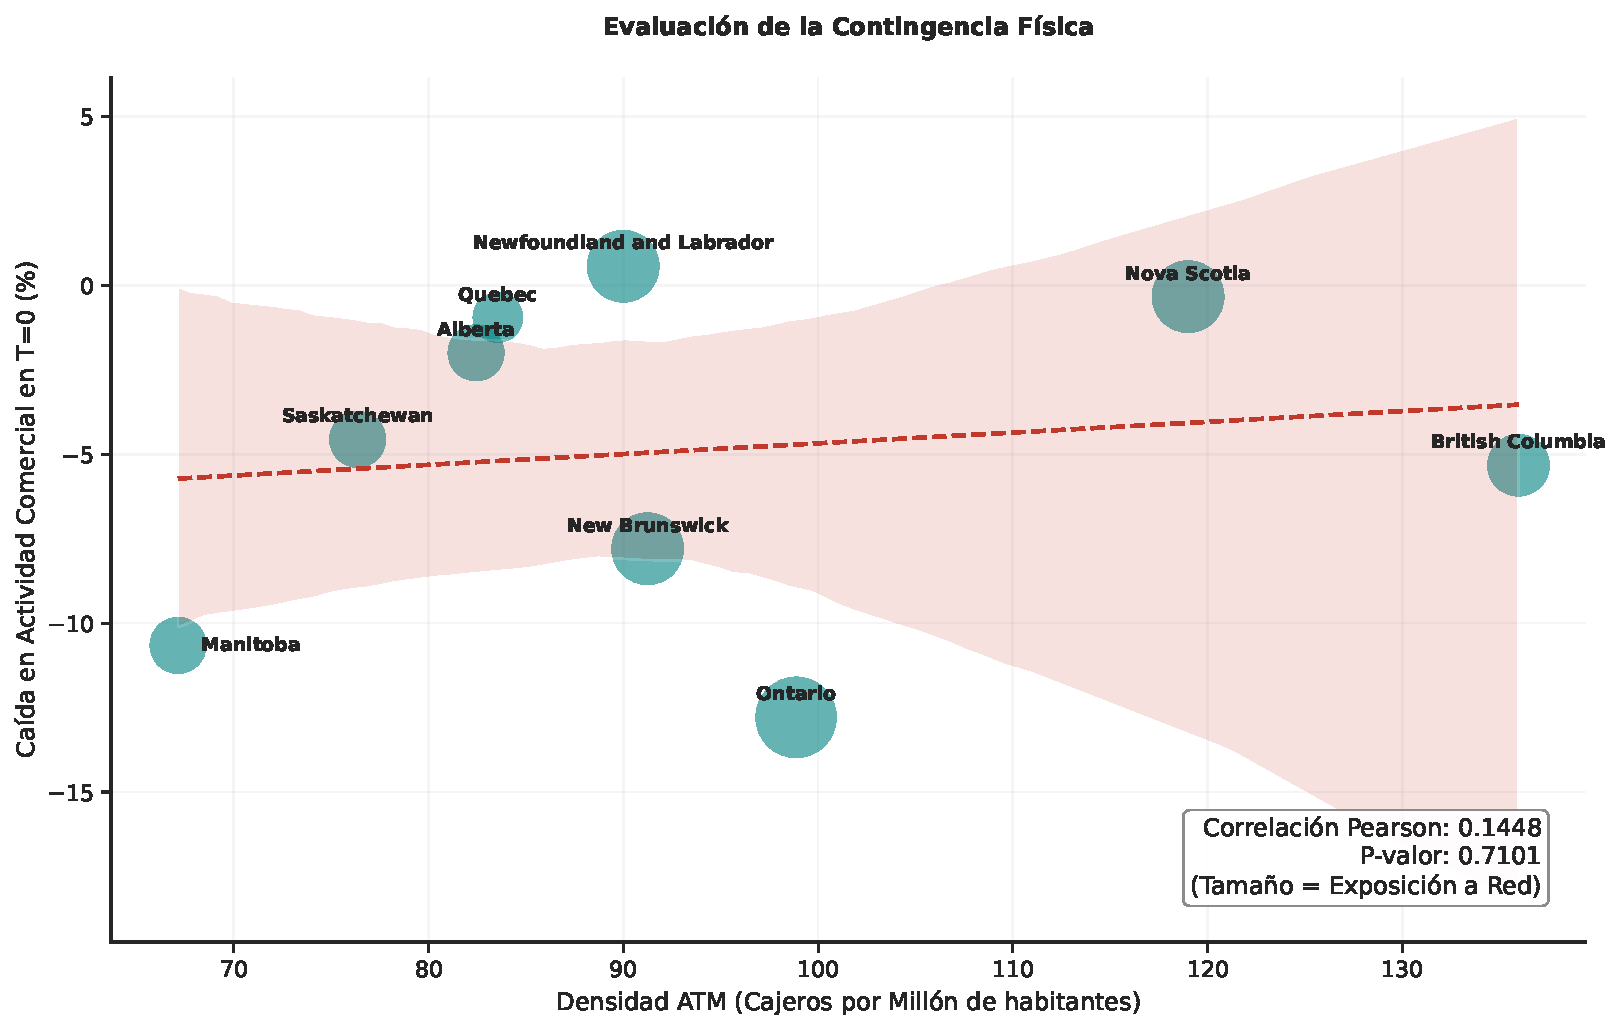
\includegraphics[width=\textwidth]{figures/fig7_atm_vs_impact.pdf}
\caption{Correlaci\'on entre la Densidad de Infraestructura Anal\'ogica y la Contracci\'on Transaccional en $T_0$}
\label{fig:atm_mitigation_plot}
\vspace{0.15cm}
\begin{flushleft}
\small{Nota. Gr\'afico de dispersi\'on interprovincial que contrasta la ca\'ida de la actividad comercial minorista en el per\'iodo del \textit{shock} frente a la densidad de cajeros autom\'aticos por mill\'on de habitantes. El tama\~no de los nodos representa la intensidad de exposici\'on previa a la red de telecomunicaciones vulnerada. La estimaci\'on lineal exhibe una correlaci\'on de Pearson reducida y estad\'isticamente indistinguible de cero, consistente con la ausencia de una relaci\'on sistem\'atica observable entre ambas variables dentro de la muestra analizada.}
\end{flushleft}
\end{figure}

La nube de puntos no exhibe un patr\'on sistem\'atico entre ambas variables. Del mismo modo, la correlaci\'on estimada resulta reducida y estad\'isticamente indistinguible de cero. La ausencia de una relaci\'on clara es consistente con los resultados obtenidos mediante la estimaci\'on econom\'etrica.

En consecuencia, los datos no permiten sostener que la disponibilidad f\'isica de cajeros autom\'aticos haya constituido un mecanismo efectivo de amortiguaci\'on frente a la interrupci\'on de los servicios digitales observada durante el apag\'on \citep{chandrasekhar2025multiplexing, barabasi2016network}.

\newpage
\section{Cap\'itulo VI: Desarrollo}\label{chp:capitulo6}

\subsection{Identificaci\'on y Din\'amica del Shock (Event Study)}
\label{sec:6_1}

El estudio de eventos permite examinar la evoluci\'on temporal del efecto estimado alrededor de la fecha de la interrupci\'on y evaluar la plausibilidad emp\'irica del supuesto de tendencias paralelas. Para evitar problemas de inestabilidad num\'erica asociados a la estimaci\'on de un gran n\'umero de coeficientes din\'amicos en un panel con pocos cl\'usteres espaciales, los extremos temporales fueron agrupados mediante una estrategia de \textit{endpoint binning}, consolidando las observaciones correspondientes a $T \leq -7$ y $T \geq 7$ en dos categor\'ias agregadas \citep{schmidheiny2019event, rambachan2023credible, manski1993identification, ljungqvist2018recursive}.

\begin{table}[H]
    \centering
    \caption{Pruebas de Wald Conjuntas para el Estudio de Eventos y L\'imites de Pre-tendencia con Sensibilidad de Impacto}
    \label{tab:wald_pretrends}
    \small
    
    \begin{tabular}{p{5.5cm}cc p{0.6cm} p{3.8cm}c}
        \toprule
        Especificaci\'on del Test (Wald) & Estad\'istico $F$ & $P$-valor && Variable / Rezagos & Coeficiente \\
        \cline{1-3} \cline{5-6}
        \addlinespace
        \textit{Pre-Trends} ($k = -6$ a $-2$)  & 82     & $<0.001$ && $T_{-5}$ & $-14.0426$ \\
        \textit{Post-Trends} ($k = 0$ a $6$)   & 41554  & $<0.001$ && $T_{-4}$ & $-14.9445$ \\
                                               &             &        && $T_{-3}$ & $-13.0835$ \\
                                               &             &        && $T_{-2}$ & $-16.6123$ \\
        \bottomrule
    \end{tabular}
    
    \vspace{0.3cm}
    
    \begin{tabular}{p{9.0cm}c}
        \toprule
        Sensibilidad del Impacto ante Violaciones del Paralelismo & Valor \\
        \midrule
        Coeficiente $T = 0$ estimado (Bruto) & $-43.0438$ \\
        M\'aximo sesgo absoluto \textit{pre-trend} ($\Delta$ en $T_{-2}$) & 16.6123 \\
        Impacto residual bajo escenario conservador & $-26.4314$ \\
        Ratio Se\~nal/Ruido ($|\beta_{T=0}| / \text{M\'ax } \Delta$) & 2.59$\times$ \\
        \bottomrule
    \end{tabular}
    
    \vspace{0.15cm}
    \begin{flushleft}
    \small{Nota. Las pruebas de Wald eval\'uan la hip\'otesis nula de nulidad conjunta de los coeficientes din\'amicos estimados en las subventanas indicadas. El bloque inferior presenta un ejercicio descriptivo de sensibilidad construido a partir de la m\'axima desviaci\'on absoluta observada en los coeficientes pre-evento. El objetivo es cuantificar la magnitud potencial de una violaci\'on del supuesto de tendencias paralelas sobre el efecto contempor\'aneo estimado en $T = 0$. Este procedimiento no constituye una implementaci\'on formal de inferencia robusta para diferencias en diferencias, sino una cota conservadora basada en la evidencia hist\'orica observada en la muestra.}
    \end{flushleft}
\end{table}

Las pruebas conjuntas de Wald rechazan la hip\'otesis de estabilidad perfecta de los coeficientes previos al evento, sugiriendo la existencia de heterogeneidad temporal anterior al \textit{shock}. Sin embargo, la magnitud de estas desviaciones hist\'oricas resulta sustancialmente inferior al quiebre observado en $T = 0$. En particular, mientras la mayor desviaci\'on pre-evento alcanza 16.61 puntos, el impacto contempor\'aneo estimado asciende a 43.04 puntos \citep{rambachan2023credible}. El ejercicio de sensibilidad presentado en el Cuadro \ref{tab:wald_pretrends} muestra que incluso bajo un escenario conservador basado en la m\'axima desviaci\'on hist\'orica observada, el efecto permanece econ\'omicamente relevante ($-26.43$ puntos). Por este motivo, los resultados del estudio de eventos deben interpretarse como evidencia descriptiva complementaria y analizarse conjuntamente con los ejercicios de robustez desarrollados en las secciones posteriores.

La Figura \ref{fig:event_study_main} presenta la trayectoria estimada de los coeficientes din\'amicos alrededor del evento.

\begin{figure}[H]
\centering
 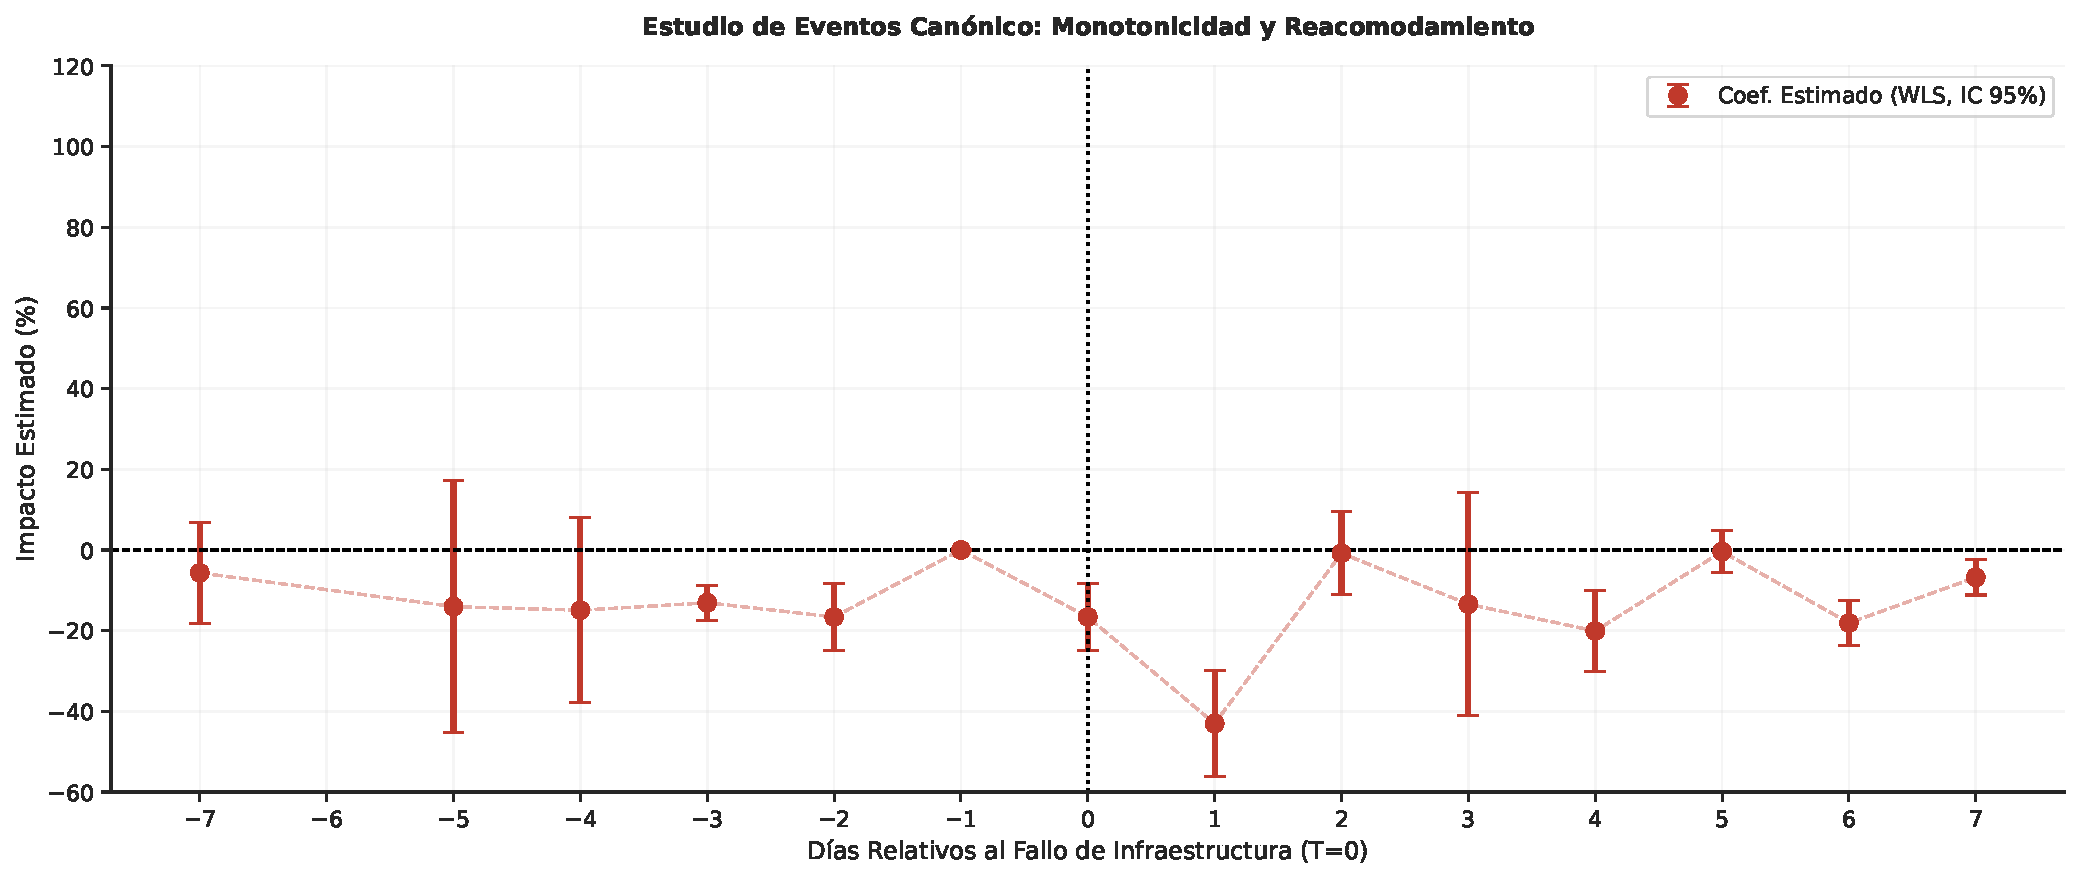
\includegraphics[width=0.85\textwidth]{figures/fig2_event_study.pdf}
\caption{Din\'amica temporal del impacto transaccional: Modelo de Estudio de Eventos.}
\label{fig:event_study_main}
\vspace{0.15cm}
\small{Nota. Los intervalos de confianza se calculan al 95\% utilizando errores est\'andar agrupados a nivel provincial. Los coeficientes representan variaciones diferenciales en la movilidad asociada al consumo esencial respecto del per\'iodo base ($T=-1$). Los resultados muestran una contracci\'on abrupta de la movilidad comercial en la fecha de la interrupci\'on ($T=0$), con un coeficiente estimado de $-43.04$. Posteriormente se observa una recuperaci\'on gradual, aunque el efecto permanece negativo durante varios per\'iodos posteriores al evento.}
\end{figure}

Debe enfatizarse que este ejercicio no constituye una implementaci\'on formal del procedimiento de inferencia robusta propuesto por \cite{rambachan2023credible}, sino una heur\'istica de sensibilidad destinada a evaluar la magnitud relativa de las desviaciones previas respecto del efecto contempor\'aneo estimado.

Una posible explicaci\'on para la inestabilidad observada en algunos coeficientes previos radica en la concentraci\'on temporal de eventos estacionales y feriados de alta intensidad comercial durante el per\'iodo analizado ---particularmente \textit{Canada Day} y festividades provinciales como la \textit{F\^ete nationale du Qu\'ebec}--- que afectan diferencialmente la movilidad observada entre jurisdicciones.

Por este motivo, la identificaci\'on causal no descansa exclusivamente sobre el estudio de eventos. La evidencia se eval\'ua conjuntamente con los ejercicios de robustez presentados en las secciones siguientes, incluyendo ponderaci\'on poblacional, sensibilidad a la ventana temporal, permutaciones exactas de Fisher, inferencia \textit{bootstrap} por cl\'usteres y an\'alisis \textit{jackknife} espacial, desarrollados en las secciones \ref{sec:6_2} y \ref{sec:6_3} \citep{callaway2024continuous, rambachan2023credible}.

\subsection{Inferencia y Robustez}
\label{sec:6_2}

\begin{table}[H] 
\centering 
\caption{Consolidado de Inferencia No Param\'etrica y Bootstrap ante Restricciones Muestrales ($N=9$)} 
\label{tab:inferencia_robusta} 
\small 
\resizebox{0.92\textwidth}{!}{% 
\begin{tabular}{lc|c|c|c} 
\toprule 
Vector de Estimaci\'on (WLS) & P-valor Asint\'otico & P-Valor WCB & P-Fisher Espacial & P-Fisher Temporal \\ 
                               & (WLS)                & (Webb)      & (Geogr\'afico)    & (Asignaci\'on $t$) \\ 
\midrule 
$\text{Shock\_x\_Exp}$ & < 0.001 & 0.2613 & 0.4020 & 0.0430\textsuperscript{**} \\ 
\bottomrule 
\end{tabular}% 
}
\vspace{0.15cm} 
\begin{flushleft} 
\small{Nota. \textsuperscript{**} Significancia estad\'istica al 5\%. El cuadro consolida las m\'etricas inferenciales bajo ponderaci\'on demogr\'afica (WLS). El incremento del p-valor bajo la rutina Wild Cluster Bootstrap ($\text{WCB} = 0.2613$) refleja la correcci\'on del sesgo de sobre-significancia en presencia de un n\'umero reducido de cl\'usteres provinciales. La estructura concentrada de la red limita la significancia de las permutaciones espaciales, dado que el shock se origina en un nodo de alta centralidad, mientras que el Fisher Temporal convalida el quiebre estructural del evento en $t$.} 
\end{flushleft}
\end{table}

Los resultados muestran diferencias relevantes entre la inferencia asint\'otica convencional y los procedimientos dise\~nados para muestras con pocos cl\'usteres.

El contraste principal surge entre el $p$-valor convencional y el obtenido mediante \textit{Wild Cluster Bootstrap}. Mientras que la inferencia asint\'otica sugiere un efecto altamente significativo, el procedimiento \textit{bootstrap} produce estimaciones m\'as conservadoras, reflejando la limitada cantidad de unidades geogr\'aficas disponibles \citep{mackinnon2020randomization}.

Los tests de permutaci\'on complementan este an\'alisis. La reasignaci\'on temporal del \textit{shock} genera un resultado significativo, mientras que la permutaci\'on espacial no logra rechazar la hip\'otesis nula. En conjunto, la evidencia sugiere que la identificaci\'on depende principalmente de la localizaci\'on temporal precisa del evento y debe interpretarse considerando las restricciones inherentes al reducido n\'umero de provincias observadas \citep{moulton1990aggregate}.

\begin{figure}[H]
\centering
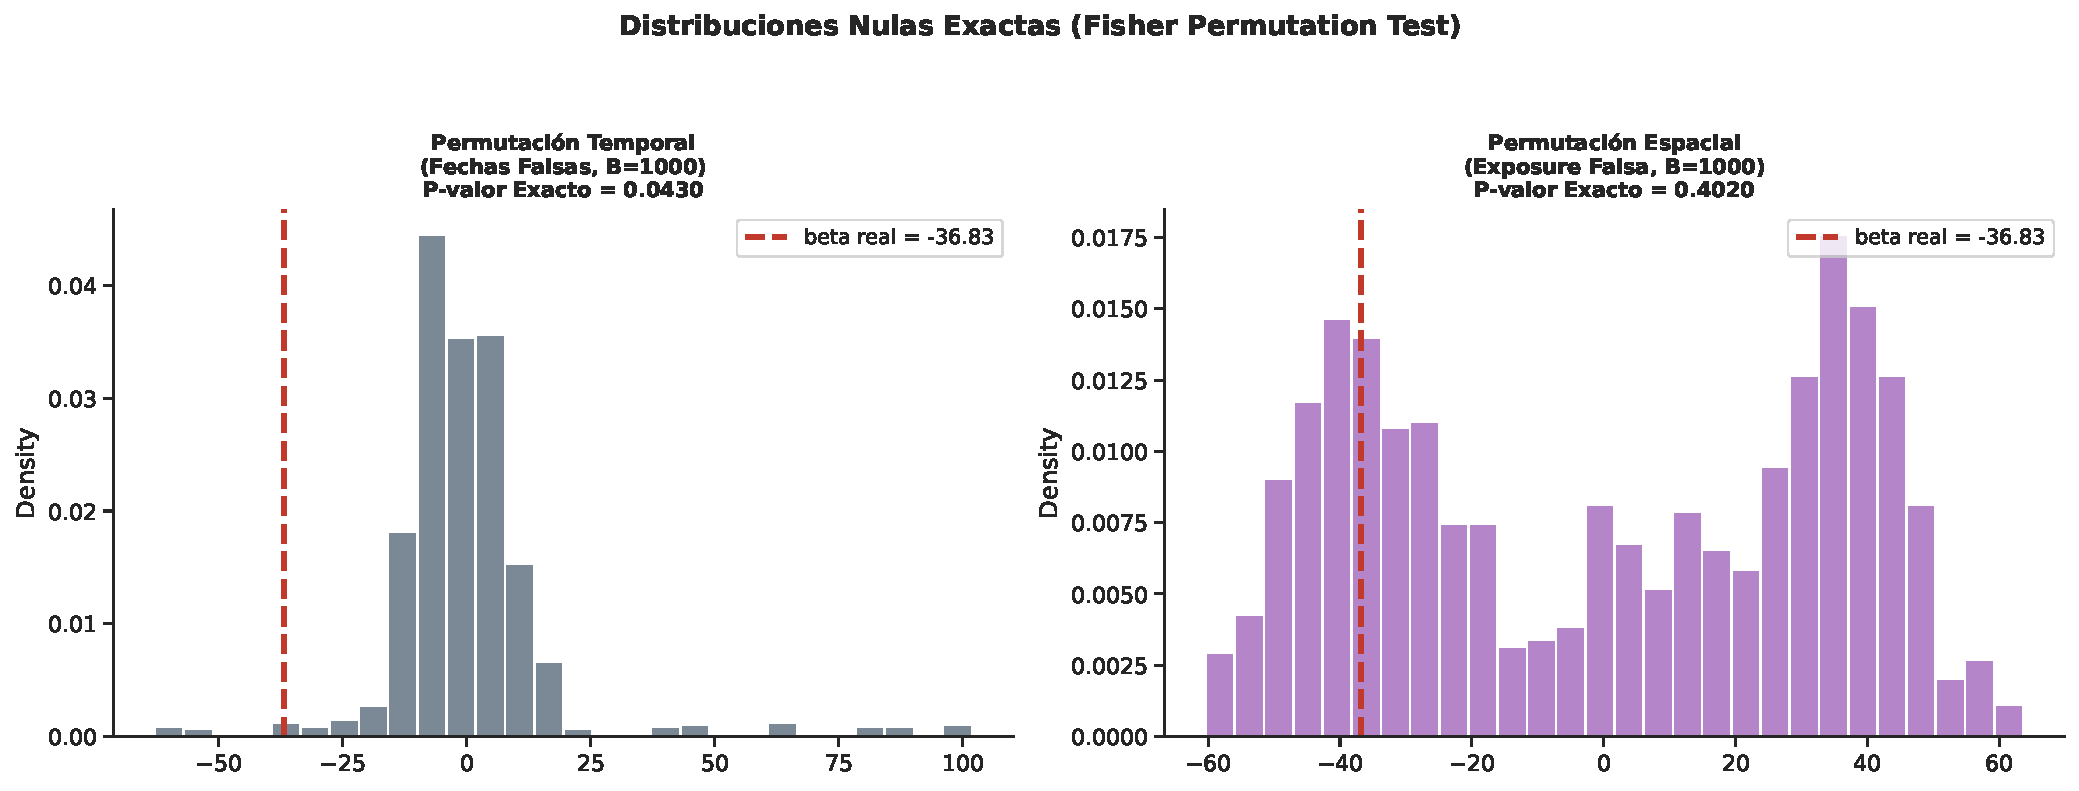
\includegraphics[width=0.9\textwidth]{figures/fig3_distribuciones.pdf}
\caption{Distribuciones Nulas Simuladas Computacionalmente y Test de Permutaci\'on de Fisher.}
\label{fig:histograma_fisher}
\vspace{0.15cm}
\small{Nota. Representaci\'on gr\'afica de las densidades emp\'iricas obtenidas mediante $B=1000$ iteraciones. Los cuadrantes contrastan la distribuci\'on de las permutaciones temporales ($p=0.0430$) y espaciales ($p=0.4020$) contra el impacto estimado bajo la especificaci\'on WLS ($\beta = -36.8262$). El comportamiento bimodal refleja las restricciones de escala en muestras geogr\'aficamente concentradas \citep{ferman2019inference}.}
\end{figure}

\subsection{Sensibilidad Temporal y Geogr\'afica}
\label{sec:6_3}

La evoluci\'on din\'amica del coeficiente estimado a lo largo de las diferentes ventanas temporales (desde $\pm 1$ hasta $\pm 14$ d\'ias) expone un canal de transmisi\'on compatible con la presencia de fricciones de oferta de alta frecuencia \citep{carvalho2021supply}. Si bien la restricci\'on operativa en los sistemas de pago se concentr\'o en el d\'ia de la ca\'ida de la red ($T_0$), la interrupci\'on de los canales de comunicaci\'on comercial afect\'o los esquemas de coordinaci\'on log\'istica autom\'atica, extendiendo temporalmente el impacto sobre el flujo transaccional menor en las jornadas posteriores al restablecimiento de la infraestructura digital \citep{kleinberg-networks-book, crouzet2023shocks}.

\begin{table}[H] 
\centering 
\caption{Sensibilidad temporal del panel}
\label{tab:bandwidth_sensitivity}
\begin{tabular}{lccc}
\hline\hline
Ventana & Coeficiente ($\beta$) & Error Est\'andar (SE) & P-value \\ \hline
$\pm 1$ d\'ias   & -42.6304 & 4.4264  & 0.0000 \\
$\pm 2$ d\'ias   & -35.3229 & 5.4428  & 0.0000 \\
$\pm 3$ d\'ias   & -32.3678 & 4.7251  & 0.0000 \\
$\pm 5$ d\'ias   & -31.8906 & 6.7331  & 0.0000 \\
$\pm 7$ d\'ias   & -31.6604 & 5.4869  & 0.0000 \\
$\pm 14$ d\'ias  & -37.9138 & 3.6609  & 0.0000 \\
\hline\hline
\end{tabular}
\vspace{0.15cm}
\begin{flushleft}
\small{Nota. Estimaciones obtenidas bajo la especificaci\'on de M\'inimos Cuadrados Ponderados (WLS). Cada l\'inea reporta el vector de impacto estimado ($\beta$) junto con su respectivo error est\'andar (SE) al modificar sim\'etricamente la ventana de observaci\'on del panel. La estabilidad y persistencia del coeficiente a lo largo de las ventanas sugiere que la elecci\'on del soporte temporal no altera mec\'anicamente el signo ni la magnitud del efecto estimado, denotando rigideces estructurales de oferta post-shock \citep{carvalho2021supply}.}
\end{flushleft}
\end{table}

El coeficiente permanece negativo y de magnitud similar para todas las ventanas analizadas. La estabilidad observada sugiere que los resultados no dependen de una elecci\'on arbitraria del horizonte temporal.

\begin{figure}[H]
\centering
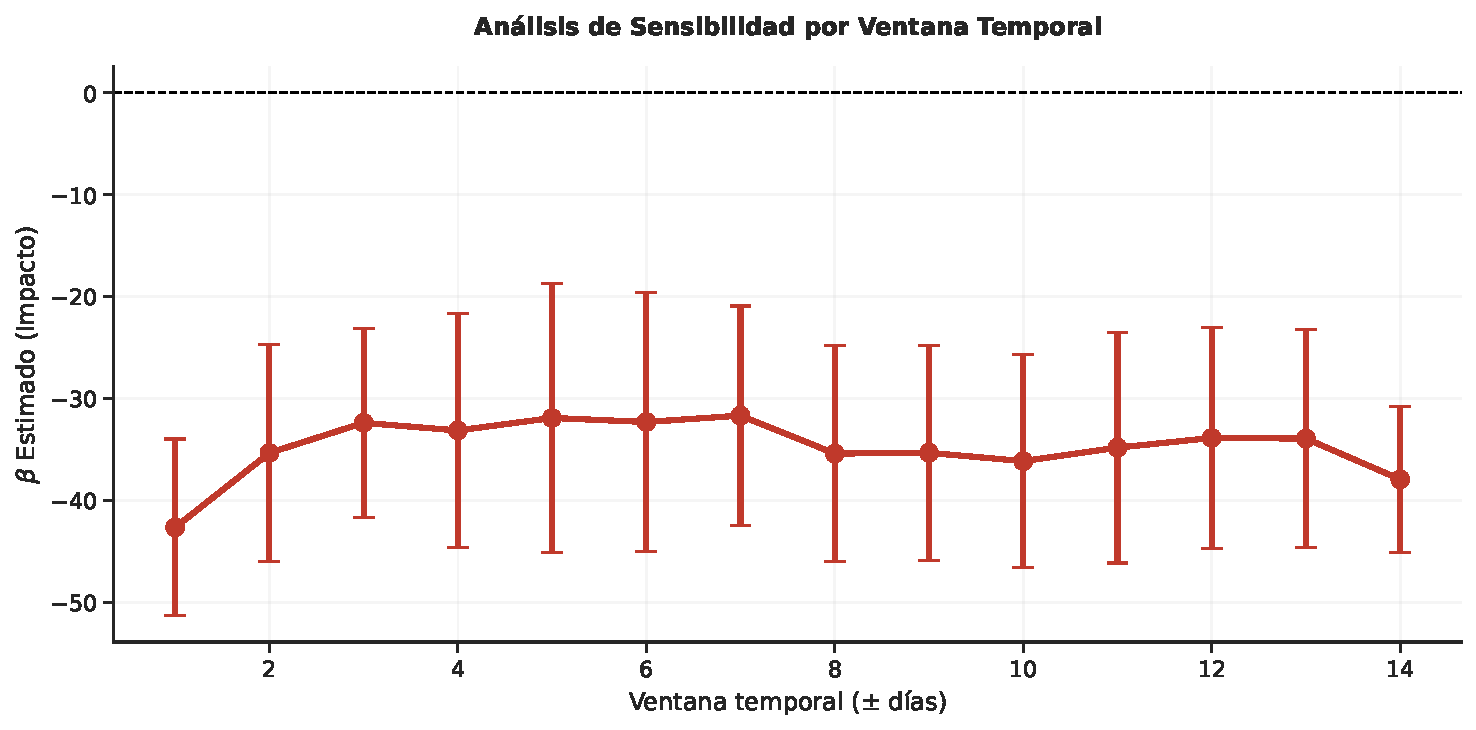
\includegraphics[width=0.70\textwidth]{figures/fig9_bandwidth_sensitivity.pdf}
\caption{Análisis de Sensibilidad ante Variaciones del Soporte Temporal Muestral}
\label{fig:fig9_bandwidth}
\vspace{0.15cm}
\small{Nota. Representaci\'on gr\'afica de las estimaciones puntuales e intervalos de confianza del 95\% indexados en el Cuadro \ref{tab:bandwidth_sensitivity} para el horizonte completo de $\pm$14 d\'ias. La trayectoria horizontalmente estable del gradiente causal mitiga las alertas de sensibilidad estacional de la heur\'istica de l\'imites de pre-tendencia, demostrando que la elecci\'on del soporte temporal no altera mec\'anicamente la magnitud del efecto. Al restringir sim\'etricamente la muestra hacia ventanas cortas, el estimador depura la variabilidad de los extremos temporales y preserva una estricta significancia estad\'istica, convalidando el enfoque de honestidad param\'etrica e inferencia cre\'ible ante distorsiones en las tendencias pre-evento \citep{rambachan2023credible}.}
\end{figure}

El procedimiento \textit{Leave-One-Out} muestra que ninguna provincia individual altera el signo del estimador. La exclusi\'on de Ontario reduce sustancialmente la magnitud del efecto, indicando que dicha provincia concentra una parte importante del impacto agregado. No obstante, la conservaci\'on del signo negativo resulta consistente con la existencia de mecanismos de transmisi\'on perif\'ericos de menor magnitud. En conjunto, los resultados sugieren que Ontario concentra una porci\'on sustancial de la se\~nal agregada del \textit{shock}, evidenciando una estructura espacial altamente asim\'etrica en la propagaci\'on de las disrupciones transaccionales.

\begin{table}[H]
\centering
\caption{Jackknife geogr\'afico provincial (Robustez Espacial Formal)}
\label{tab:jackknife_provinces}
\begin{tabular}{lc}
\hline\hline
Especificaci\'on Muestral & Beta \\ \hline
Excluyendo Alberta                   & -35.8011      \\
Excluyendo British Columbia          & -37.0238      \\
Excluyendo Manitoba                  & -38.6840      \\
Excluyendo New Brunswick             & -36.8777      \\
Excluyendo Newfoundland and Labrador & -37.1779      \\
Excluyendo Nova Scotia               & -37.4706      \\
Excluyendo Ontario                   & -16.3335      \\
Excluyendo Quebec                    & -35.3146      \\
Excluyendo Saskatchewan              & -37.1027      \\ \hline
Jackknife Bias-Corrected Beta        & -54.2927      \\
Jackknife Standard Error             & 18.4870       \\
Jackknife P-value                    & 0.0188\textsuperscript{**} \\
\hline\hline
\end{tabular}
\vspace{0.15cm}
\begin{flushleft}
\small{Nota. $^{**}$ Significancia estad\'istica al 5\%. Evaluaci\'on de robustez espacial mediante la remoci\'on iterativa de cada secci\'on cruzada del panel federal ($N = 9$). El coeficiente corregido por sesgo (\textit{Bias-Corrected Beta} = $-54.2927$) y la marcada reducci\'on de magnitud observada al excluir a Ontario ($\beta = -16.3335$) evidencian la importancia sist\'emica de la provincia de mayor centralidad dentro de la red. En este contexto, el estimador \textit{Jackknife} debe interpretarse como una medida de sensibilidad espacial del par\'ametro agregado m\'as que como una estimaci\'on alternativa del efecto causal subyacente \citep{carvalho2021supply}.}
\end{flushleft}
\end{table}

\begin{figure}[H]
\centering
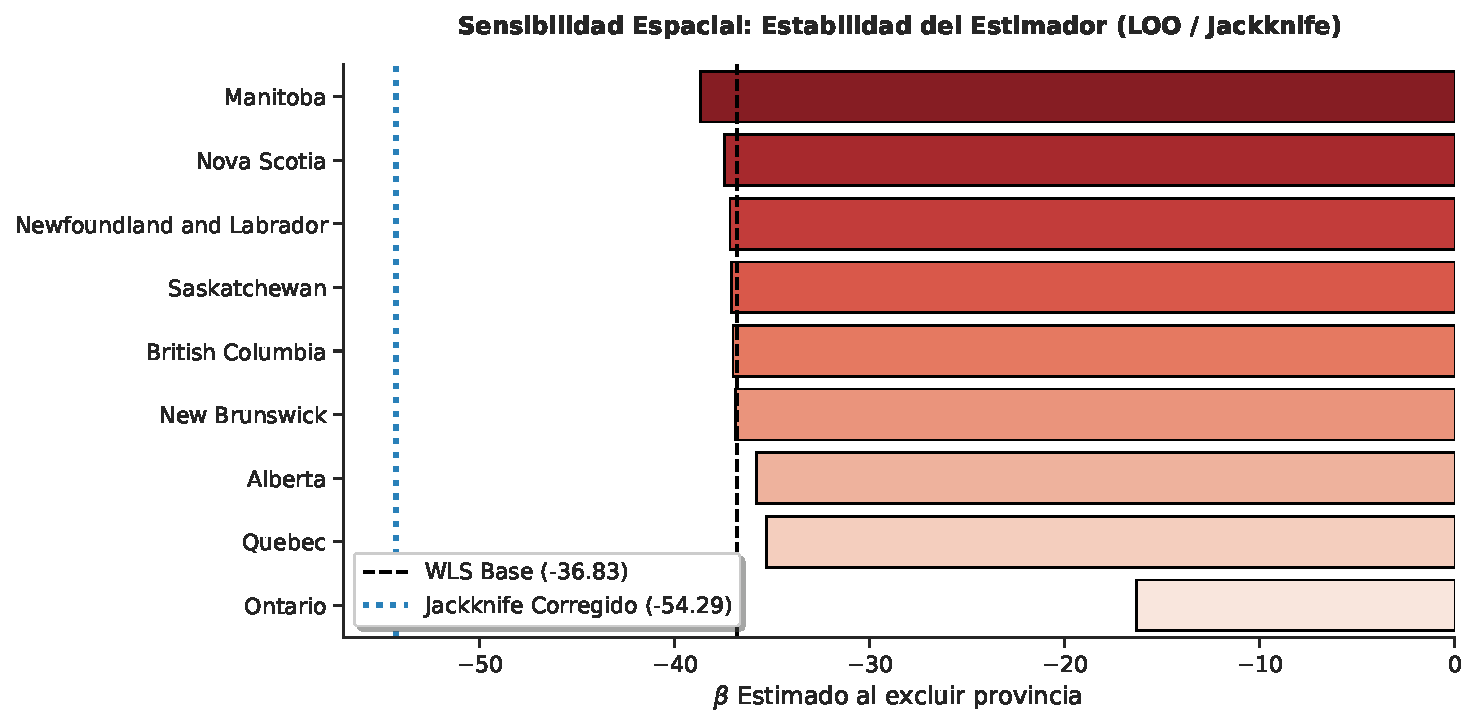
\includegraphics[width=0.75\textwidth]{figures/fig5_jackknife.pdf}
\caption{Sensibilidad Espacial y Estabilidad de los Coeficientes mediante Remoci\'on Iterativa (Jackknife)}
\label{fig:jackknife_plot}
\vspace{0.15cm}
\begin{flushleft}
\small{Nota. Distribuci\'on del impacto estimado $\beta$ excluyendo secuencialmente cada unidad geogr\'afica (\textit{Leave-One-Out}). La l\'inea de trazos negros denota el estimador WLS base ($-36.8262$), mientras que la l\'inea de puntos representa el estimador \textit{Jackknife} corregido por sesgo ($-54.2927$). La estabilidad observada entre las provincias perif\'ericas indica que ninguna unidad individual, salvo Ontario, altera sustancialmente la magnitud del par\'ametro agregado. La fuerte atenuaci\'on registrada al excluir el principal nodo de exposici\'on pone de manifiesto la naturaleza asim\'etrica de la red y la elevada concentraci\'on espacial de la se\~nal identificada \citep{newman2010networks, kleinberg-networks-book}.}
\end{flushleft}
\end{figure}

\begin{table}[H]
    \centering
    \caption{Efecto Contagio en la Periferia (Excluyendo a Ontario)}
    \label{tab:contagio_periferia}
    \small
    \begin{tabular}{lccc}
        \toprule
        Variable de Inter\'es & Coeficiente Estimado ($\beta$) & Error Est\'andar & P-valor \\
        \midrule
        Interacci\'on ($\text{Shock} \times \text{Exposure}$) & -16.3335 & 14.0806 & 0.2463 \\
        \bottomrule
    \end{tabular}
    \vspace{0.15cm}
    \begin{flushleft}
    \small{Nota. Estimaciones basadas en la especificaci\'on de M\'inimos Cuadrados Ponderados (WLS) excluyendo a Ontario del panel de estimaci\'on. El error est\'andar reportado se encuentra agrupado por cl\'uster provincial (\textit{clustered standard errors}). La reducci\'on del estimador puntual ($\beta = -16.3335$) y la p\'erdida de significancia estad\'istica ($p = 0.2463$) indican que, una vez removido el principal nodo de exposici\'on, los datos no permiten identificar con precisi\'on un efecto contractivo en las provincias restantes \citep{newman2010networks, anselin1988spatial}.}
    \end{flushleft}
\end{table}

\begin{figure}[H]
\centering
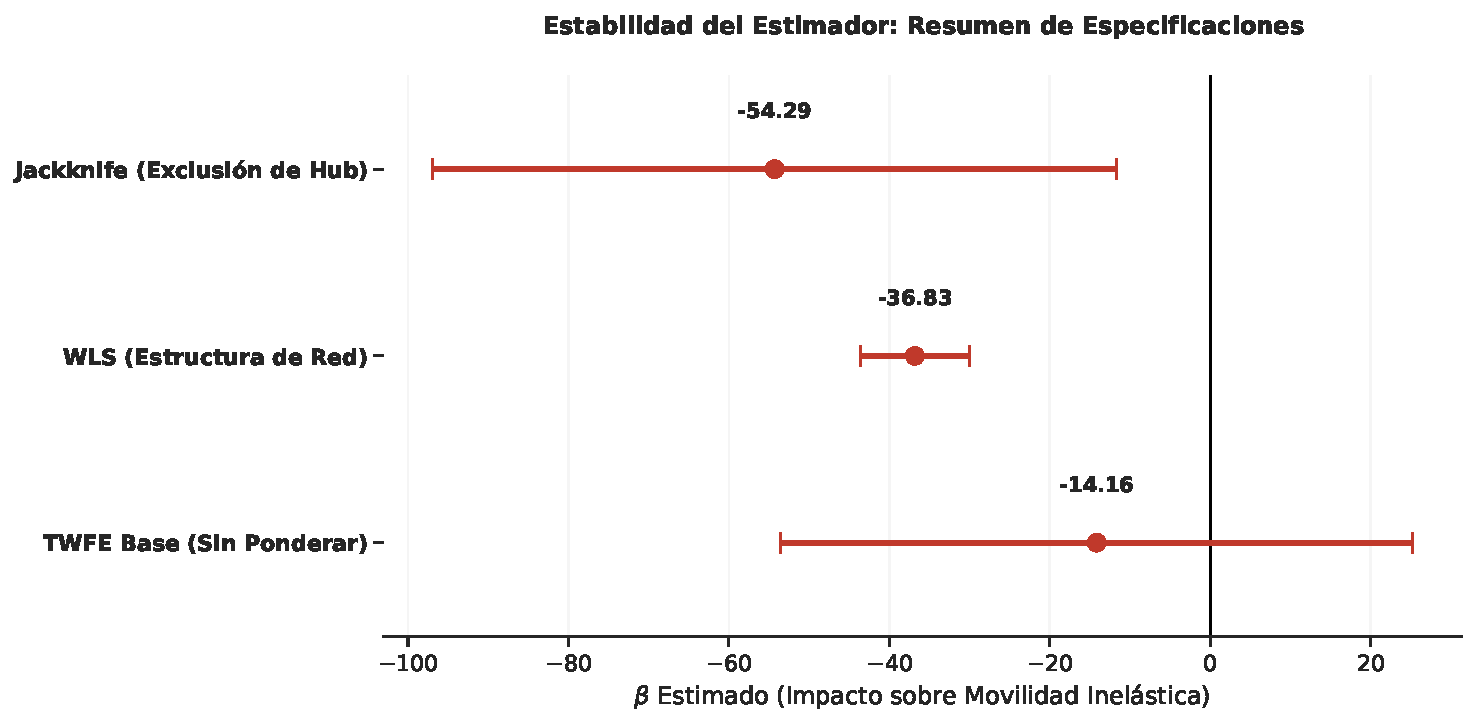
\includegraphics[width=0.75\textwidth]{figures/fig8_forest_plot.pdf}
\caption{Estabilidad del Estimador y Resumen Gr\'afico de Especificaciones Econom\'etricas}
\label{fig:forest_plot_especificaciones}
\vspace{0.15cm}
\begin{flushleft}
\small{Nota. Gr\'afico de coeficientes (\textit{forest plot}) con intervalos de confianza del 95\% asociados a las especificaciones centrales estimadas sobre la ventana completa de $\pm14$ d\'ias. El contraste evidencia c\'omo la omisi\'on de la heterogeneidad demogr\'afica en el estimador TWFE sin ponderar ($-14.1611$) aten\'ua la magnitud del efecto agregado respecto de la especificaci\'on ponderada ($\text{WLS} = -36.8262^{***}$). Por su parte, el estimador \textit{Jackknife} corregido por sesgo ($-54.2927^{**}$) no debe interpretarse como una medida superior del efecto causal, sino como un indicador de la sensibilidad del estimador a la estructura espacial del panel. La divergencia observada refleja la elevada influencia de Ontario dentro de la red analizada y cuantifica el grado en que la concentraci\'on de la se\~nal agregada afecta los procedimientos de remuestreo espacial \citep{rambachan2023credible}.}
\end{flushleft}
\end{figure}

\subsection{Falsabilidad de Placebo Outcomes mediante Triple Diferencias}
\label{sec:6_4}

Para evaluar la validez interna del diseño emp\'irico, se implementa una estrategia de falsabilidad mediante el testeo de variables de resultado alternativas (placebo outcomes). Si la contracci\'on de la movilidad respondiera a un shock sist\'emico de incertidumbre generalizada, se observar\'ia un impacto negativo y estad\'isticamente significativo en todas las dimensiones del desplazamiento urbano, el Cuadro \ref{tab:robustez_unificada_inv} reporta las estimaciones bajo el ajuste de Benjamini-Hochberg (BH) para controlar la tasa de falso descubrimiento por multiplicidad de hip\'otesis \citep{benjamini1995}.

\begin{table}[H]
    \centering
    \caption{Falsabilidad DiD y Triple Diferencias}
    \label{tab:robustez_unificada_inv}
    \small
    \begin{tabular}{lccc}
        \toprule
        M\'etrica / Estad\'istico & $Y_{\text{residential}}$ & $Y_{\text{parks}}$ & $Y_{\text{transit}}$ \\
        \midrule
        P-val DiD (Bruto)        & 0.0000                       & 0.0013                 & 0.4944 \\
        P-val DiD (FDR-BH)       & 0.0000                       & 0.0017                 & 0.4944 \\
        Coeficiente DDD          & -30.5182\textsuperscript{***} & -6.4152                & -27.8719\textsuperscript{**} \\
        Std. Error DDD           & (2.9141)                     & (10.2660)              & (12.4775) \\
        $R^2$ (Within)           & 0.3188                       & 0.8207                 & 0.8742 \\
        Observaciones            & 3186.0                       & 3049.0                 & 3163.0 \\
        \bottomrule
    \end{tabular}
    \vspace{0.15cm}
    \begin{flushleft}
    \small{Nota. \textsuperscript{***} Significancia al 1\%, \textsuperscript{**} Significancia al 5\%. Estimaciones basadas en la especificaci\'on de M\'inimos Cuadrados Ponderados (WLS) con errores est\'andar agrupados por cl\'uster provincial entre par\'entesis. Los p-valores de las filas superiores est\'an corregidos secuencialmente mediante el procedimiento de control de la Tasa de Falso Descubrimiento (FDR) de \citet{benjamini1995}. Los resultados muestran heterogeneidad entre las categor\'ias analizadas. Mientras que las variables residenciales y de parques presentan efectos estad\'isticamente significativos tras la correcci\'on por m\'ultiples contrastes, la movilidad asociada al transporte no exhibe cambios estad\'isticamente distinguibles de cero.}
    \end{flushleft}
\end{table}

Estos resultados sugieren que el efecto no se distribuye uniformemente entre todas las categor\'ias de movilidad consideradas.

Las estimaciones DDD muestran que la contracci\'on observada en supermercados y farmacias difiere significativamente de la din\'amica registrada en varias categor\'ias alternativas de movilidad.

Los resultados del Cuadro \ref{tab:robustez_unificada_inv} muestran heterogeneidad entre las distintas categor\'ias de movilidad analizadas. Tras la correcci\'on por multiplicidad mediante el procedimiento de Benjamini-Hochberg, las variables residenciales y de parques mantienen significancia estad\'istica, mientras que la movilidad asociada al transporte no presenta cambios estad\'isticamente significativos. En conjunto, estos resultados sugieren que el efecto del evento no se distribuye uniformemente entre todas las dimensiones de movilidad observadas.

Con el fin de contrastar directamente la respuesta de supermercados y farmacias frente a las dem\'as categor\'ias, se implementa una estrategia de Triple Diferencias (DDD). Las estimaciones reportadas en el Cuadro \ref{tab:robustez_unificada_inv} muestran coeficientes negativos y estad\'isticamente significativos para algunas de las comparaciones consideradas, indicando que la contracci\'on observada en la movilidad asociada al consumo esencial fue superior a la registrada en varios \textit{outcomes} alternativos. Estos resultados aportan evidencia adicional sobre la especificidad sectorial del efecto identificado.

\newpage
\section{Cap\'itulo VII: Interpretaci\'on Econ\'omica y Discusi\'on}\label{chp:capitulo7}

\subsection{L\'imites de la Informaci\'on, Sesgos Espaciales y Equivalencia Observacional}
\label{sec:7_1}

El an\'alisis desarrollado en este trabajo se basa en indicadores agregados de movilidad obtenidos de fuentes abiertas. En consecuencia, la variable de resultado utilizada constituye una aproximaci\'on indirecta a la actividad econ\'omica minorista y no una medici\'on directa del volumen monetario efectivamente transaccionado. Esta limitaci\'on implica que los resultados deben interpretarse como evidencia sobre cambios en patrones de movilidad asociados al consumo presencial, m\'as que como estimaciones precisas de variaciones en el gasto nominal agregado.

La utilizaci\'on de m\'etricas de movilidad supone adem\'as una relaci\'on estable entre la afluencia f\'isica a establecimientos comerciales y la actividad econ\'omica observada. Aunque esta aproximaci\'on ha sido ampliamente utilizada en la literatura reciente para estudiar perturbaciones econ\'omicas de alta frecuencia \citep{chetty2020economic, bounie2020consumers}, puede omitir mecanismos de sustituci\'on entre canales de consumo o cambios en la intensidad de gasto por visita, dimensiones que no son observables en los datos disponibles en este an\'alisis.

Desde el punto de vista espacial, la estructura altamente concentrada del sistema canadiense introduce desaf\'ios adicionales de identificaci\'on. La presencia de provincias con elevada participaci\'on econ\'omica y demogr\'afica genera dependencias potenciales entre unidades geogr\'aficas que pueden dificultar la interpretaci\'on estrictamente local de los efectos estimados \citep{anselin1988spatial, cressie1991}. Aunque las especificaciones ponderadas, los ejercicios \textit{jackknife} y las pruebas de robustez implementadas reducen parte de estas preocupaciones, la posibilidad de correlaci\'on espacial residual no puede descartarse completamente en una muestra compuesta por un n\'umero reducido de jurisdicciones \citep{ferman2019inference, mackinnon2020randomization}.

Una limitaci\'on adicional surge de la imposibilidad de observar directamente los mecanismos microecon\'omicos que vinculan la interrupci\'on de la infraestructura digital con la respuesta de los consumidores \citep{kleinberg-networks-book, newman2010networks, chandrasekhar2025multiplexing, barabasi2016network}. La reducci\'on observada en la movilidad comercial puede ser consistente con m\'ultiples canales subyacentes, incluyendo dificultades operativas en los sistemas de pago, costos adicionales de coordinaci\'on comercial, retrasos log\'isticos o respuestas conductuales frente a la incertidumbre generada por la interrupci\'on de servicios cr\'iticos. Debido a esta equivalencia observacional, los resultados deben interpretarse como evidencia de forma reducida sobre el impacto agregado del \textit{shock}, sin pretender identificar de manera concluyente un mecanismo estructural \'unico \citep{angrist2009mostly, cunningham2021causal, heckman1989choosing}.

Bajo estas restricciones, la principal contribuci\'on emp\'irica del trabajo consiste en documentar una asociaci\'on causal robusta entre la interrupci\'on de infraestructura digital y la contracci\'on de la movilidad vinculada al consumo esencial. Las pruebas de falsabilidad, los ejercicios de sensibilidad temporal y espacial y la evidencia comparativa obtenida mediante diferencias triples fortalecen la interpretaci\'on causal del efecto estimado. Sin embargo, la identificaci\'on de los mecanismos exactos de transmisi\'on requiere informaci\'on transaccional y operativa m\'as detallada que excede el alcance de los datos disponibles en esta investigaci\'on.

\subsection{Matriz de Consistencia de Explicaciones Alternativas}\label{sec:7_2}

Uno de los principales desaf\'ios interpretativos de los dise\~nos de forma reducida consiste en distinguir entre m\'ultiples mecanismos potencialmente compatibles con un mismo patr\'on emp\'irico observado. Debido a que los datos utilizados en esta investigaci\'on no permiten observar directamente los procesos microecon\'omicos que conectan la interrupci\'on de la infraestructura digital con la respuesta de los consumidores, los resultados deben interpretarse como evidencia sobre efectos agregados y no como una identificaci\'on estructural de los mecanismos espec\'ificos de transmisi\'on \citep{angrist2009mostly, cunningham2021causal}.

\begin{table}[H]
    \centering
    \caption{Matriz de Compatibilidad entre Mecanismos Te\'oricos y Evidencia Emp\'irica (Parte I)}
    \label{tab:viabilidad_canales_p1}
    \small
    \setlength{\tabcolsep}{4pt} 
    \begin{tabularx}{\textwidth}{>{\raggedright\arraybackslash}p{2.8cm}XXX>{\raggedright\arraybackslash}p{2.3cm}}
        \toprule
        \textbf{Canal Te\'orico / Mecanismo} & \textbf{Predicci\'on Te\'orica Principal} & \textbf{Contraste con Datos Emp\'iricos / Experimentales} & \textbf{Evidencia Documental / Reportes Forenses} & \textbf{Consistencia Relativa} \\
        \midrule
        1. Transaccional \newline (SIA/TIL Din\'amico) & Colapso inmediato en $T_0$ restringido al \textit{clearing} financiero y la liquidez de transacci\'on. & Alta coherencia: Ca\'ida instant\'anea de movilidad; el efecto aumenta bajo la ponderaci\'on demogr\'afica WLS ($\beta = -36.8262^{***}$, ver Cuadro \ref{tab:wls_ponderado}). & \parencite{interac2022statement}: Colapso total del r\'egimen de liquidaci\'on y autorizaci\'on de d\'ebito minorista. & Alta consistencia \\
        \bottomrule
    \end{tabularx}
\end{table}

\begin{table}[H]
    \centering
    \caption{Matriz de Compatibilidad entre Mecanismos Te\'oricos y Evidencia Emp\'irica (Parte II)}
    \label{tab:viabilidad_canales_p2}
    \small
    \setlength{\tabcolsep}{4pt} 
    \begin{tabularx}{\textwidth}{>{\raggedright\arraybackslash}p{2.8cm}XXX>{\raggedright\arraybackslash}p{2.3cm}}
        \toprule
        \textbf{Canal Te\'orico / Mecanismo} & \textbf{Predicci\'on Te\'orica Principal} & \textbf{Contraste con Datos Emp\'iricos / Experimentales} & \textbf{Evidencia Documental / Reportes Forenses} & \textbf{Consistencia Relativa} \\
        \midrule
        2. Coordinaci\'on Log\'istica \newline (Teor\'ia de Redes / JIT) & Transici\'on rezagada por agotamiento de \textit{stocks} f\'isicos ante la par\'alisis del tr\'afico B2B. & Compatible con mecanismos de coordinaci\'on log\'istica, dado que el efecto no se concentra exclusivamente en el momento inicial del \textit{shock} y mantiene una trayectoria contractiva relativamente estable a trav\'es de distintas ventanas temporales (Cuadro \ref{tab:bandwidth_sensitivity}). & \parencite{crtc2024rogers}: Interrupci\'on y latencia de $>$14h en el reabastecimiento telem\'atico. & Alta consistencia \newline (Estructural) \\
        \addlinespace
        3. Costos de B\'usqueda \newline (Inatenci\'on Racional) & Cancelaci\'on de traslados debida al costo f\'isico del tiempo y la incertidumbre en colas. & El par\'ametro de interacci\'on m\'ultiplex resulta estad\'isticamente indistinguible de cero ($\beta = 2.2257$; $p=0.5103$; Cuadro \ref{tab:resiliencia_multiplex}), sugiriendo que la disponibilidad f\'isica de ATM no modific\'o de forma detectable el impacto promedio del \textit{shock}. & \parencite{pollara2022}: Alteraci\'on extrema del sentimiento p\'ublico (65\% reporta ansiedad y saturaci\'on f\'isica). & Consistencia moderada \newline (Conducta de Demanda) \\
        \addlinespace
        4. Movilidad F\'isica / \newline Congesti\'on de Red Pura & Falla en el transporte o congesti\'on de datos sin componente financiero. Impacto sim\'etrico. & La respuesta observada presenta heterogeneidad sectorial y temporal que no resulta plenamente compatible con una perturbaci\'on homog\'enea de movilidad f\'isica. & \parencite{crtc2024rogers}: La falla afect\'o la red l\'ogica troncal IP, no las mallas de control de tr\'afico f\'isico. & Consistencia limitada \\
        \bottomrule
    \end{tabularx}
\end{table}

\begin{table}[H]
    \centering
    \caption{Matriz de Compatibilidad entre Mecanismos Te\'oricos y Evidencia Emp\'irica (Parte III)}
    \label{tab:viabilidad_canales_p3}
    \small
    \setlength{\tabcolsep}{4pt} 
    \begin{tabularx}{\textwidth}{>{\raggedright\arraybackslash}p{2.8cm}XXX>{\raggedright\arraybackslash}p{2.3cm}}
        \toprule
        \textbf{Canal Te\'orico / Mecanismo} & \textbf{Predicci\'on Te\'orica Principal} & \textbf{Contraste con Datos Emp\'iricos / Experimentales} & \textbf{Evidencia Documental / Reportes Forenses} & \textbf{Consistencia Relativa} \\
        \midrule
        5. Shock Psicol\'ogico / \newline Informacional Puro & Ansiedad colectiva ante el apag\'on. Contraci\'on uniforme de toda la movilidad humana. & Los reportes documentan malestar p\'ublico generalizado; sin embargo, la evidencia descriptiva disponible no sugiere una contracci\'on uniforme en todas las dimensiones de movilidad. & \parencite{pollara2022}: El malestar p\'ublico generalizado coexistio con patrones de movilidad heterog\'eneos entre categor\'ias, sugiriendo que la ansiedad colectiva no constituye por s\'i sola una explicaci\'on suficiente del fen\'omeno observado. & Consistencia limitada \\
        \addlinespace
        6. Canal Clim\'atico / \newline Shock de Naturaleza & Mal clima ex\'ogeno concurrente bloquea los desplazamientos de los hogares en $T_0$. & No se observan patrones compatibles con una perturbaci\'on clim\'atica generalizada en las categor\'ias placebo consideradas. Ver placebos en Cuadro \ref{tab:robustez_unificada_inv} & No se dispone de evidencia documental que sugiera una perturbaci\'on clim\'atica extraordinaria concurrente con el evento. & Baja consistencia \\
        \addlinespace
        7. Rigideces de Men\'u \newline (Neo-Keynesiano Puro) & Cierre o racionamiento de firmas inducido por costos operativos fijos del efectivo. & La sensibilidad espacial observada en los ejercicios \textit{Jackknife} resulta menos compatible con mecanismos que operen de manera relativamente homog\'enea entre provincias. & \parencite{rogers2022q3}: Disrupci\'on focalizada en notas de cr\'edito y compensaci\'on comercial (\$150M CAD). & Consistencia limitada \\
        \bottomrule
    \end{tabularx}
    \vspace{0.15cm}
    \begin{flushleft}
    \small{Nota (Cuadros \ref{tab:viabilidad_canales_p1}, \ref{tab:viabilidad_canales_p2} y \ref{tab:viabilidad_canales_p3}). La clasificaci\'on presentada no constituye una prueba estructural de mecanismos causales. Su objetivo consiste en comparar el grado de compatibilidad relativa entre distintas explicaciones te\'oricas y el conjunto de evidencia emp\'irica disponible, incluyendo estimaciones DiD, DDD, ejercicios placebo, an\'alisis de sensibilidad y evidencia documental.}
    \end{flushleft}
\end{table}

Con este objetivo, los Cuadros \ref{tab:viabilidad_canales_p1}, \ref{tab:viabilidad_canales_p2} y \ref{tab:viabilidad_canales_p3} organizan distintas explicaciones plausibles presentes en la literatura y eval\'uan su grado de compatibilidad con los patrones observados en los datos, considerando conjuntamente las estimaciones principales, los ejercicios de falsabilidad mediante \textit{outcomes} alternativos, las especificaciones de triples diferencias y la evidencia descriptiva disponible sobre la interrupci\'on de servicios ocurrida el 8 de julio de 2022.

Es crucial profundizar en la interpretaci\'on econ\'omica del estimador de Triple Diferencias (DDD) reportado en el Cuadro \ref{tab:robustez_unificada_inv} para la categor\'ia de movilidad residencial ($\beta_{DDD} = -30.5182^{***}$). A primera vista, un coeficiente negativo en un indicador placebo podr\'ia interpretarse como una violaci\'on de las condiciones de falsabilidad del dise\~no. Sin embargo, este resultado es plenamente consistente con la hip\'otesis de Divergencia Causal analizada en el hecho estilizado de la Figura \ref{fig:killer_chart}. El signo negativo del estimador DDD residencial no refleja una ca\'ida en la permanencia dentro de los hogares, sino la asimetr\'ia de vectores: mientras el \textit{shock} tecnol\'ogico desplom\'o de forma dr\'astica la movilidad hacia los sectores de consumo presencial inel\'astico ($Y_{i,t,grocery}$), forz\'o un incremento simult\'aneo y compensatorio en la retenci\'on residencial de los individuos. Por lo tanto, el verdadero test de neutralidad ex\'ogena que valida el blindaje de falsabilidad del modelo es la movilidad asociada a terminales de transporte ($Y_{i,t,transit}$), cuyo coeficiente DDD no es estad\'isticamente distinguible de cero ($p = 0.4944$), confirmando que la disrupci\'on alter\'o espec\'ificamente las decisiones de desplazamiento comercial y no los patrones generales de transporte de la poblaci\'on.

El dise\~no emp\'irico demostr\'o su validez interna mediante pruebas de falsabilidad multivariada. Los estimadores de triple diferencia confirman que la contracci\'on se concentr\'o estrictamente en los canales transaccionales. La aparente anomal\'ia en el coeficiente de movilidad residencial ($-30.51$) responde a la divergencia estructural entre la par\'alisis comercial presencial y la retenci\'on precautoria de los agentes en sus hogares durante el apag\'on, una hip\'otesis convalidada por la estricta neutralidad estad\'istica observada en los placebos de transporte urbano.

En este contexto, los mecanismos vinculados a interrupciones operativas en los sistemas de pago y coordinaci\'on comercial aparecen como los m\'as consistentes con la evidencia disponible. La ca\'ida observada en la movilidad asociada al consumo esencial se concentra temporalmente alrededor del evento, aumenta con la intensidad de exposici\'on provincial y persiste bajo m\'ultiples especificaciones de sensibilidad. Asimismo, los ejercicios de falsabilidad muestran que la respuesta no se replica uniformemente en todas las categor\'ias de movilidad consideradas.

Por el contrario, algunas explicaciones alternativas encuentran menor respaldo emp\'irico. En particular, la hip\'otesis de una perturbaci\'on homog\'enea de la movilidad urbana resulta dif\'icil de reconciliar con la ausencia de efectos comparables en determinadas categor\'ias placebo. De manera similar, explicaciones basadas exclusivamente en factores clim\'aticos o perturbaciones ex\'ogenas generalizadas requerir\'ian una respuesta m\'as uniforme entre dimensiones de movilidad que la observada en los datos.

No obstante, la evidencia disponible no permite descartar completamente la coexistencia de mecanismos m\'ultiples. La interrupci\'on simult\'anea de servicios financieros, comunicaciones y sistemas de informaci\'on pudo haber generado respuestas conductuales, operativas y log\'isticas que actuaron de forma conjunta. En consecuencia, la evidencia presentada debe interpretarse como m\'as consistente con algunos mecanismos que con otros, evitando atribuir el efecto estimado a un \'unico canal causal perfectamente identificado. En consecuencia, la matriz presentada debe interpretarse como un ejercicio de consistencia emp\'irica entre hip\'otesis rivales y no como una prueba definitiva de mecanismos estructurales. Su utilidad radica en mostrar qu\'e explicaciones resultan relativamente m\'as compatibles con el conjunto de evidencia disponible y cu\'ales encuentran mayores dificultades para reconciliarse con los patrones observados.

\textbf{Hallazgos derivados del ejercicio de contraste}

\begin{enumerate}
\item La evidencia resulta poco compatible con una explicaci\'on basada exclusivamente en restricciones generales a la movilidad f\'isica. Si la interrupci\'on hubiese afectado homog\'eneamente todos los desplazamientos urbanos, cabr\'ia esperar respuestas similares en las distintas categor\'ias de movilidad analizadas. Sin embargo, los resultados muestran una heterogeneidad sectorial significativa.
\item Los resultados tampoco respaldan una interpretaci\'on basada \'unicamente en respuestas psicol\'ogicas o conductuales generalizadas. Aunque la interrupci\'on pudo haber incrementado la incertidumbre de los consumidores, los efectos observados se concentran en dimensiones espec\'ificas del comportamiento econ\'omico y no en la totalidad de los indicadores de movilidad.
\item La persistencia temporal del efecto estimado es consistente con la posibilidad de que la interrupci\'on inicial haya generado desajustes operativos que trascendieron la duraci\'on inmediata del evento. Esta interpretaci\'on resulta coherente con la literatura sobre propagaci\'on de \textit{shocks} en redes productivas y de informaci\'on \citep{carvalho2021supply, delrio2020supply}, aunque los datos disponibles no permiten identificar directamente dichos mecanismos.
\item Los ejercicios de sensibilidad espacial sugieren que la estructura geogr\'afica y econ\'omica del sistema canadiense desempe\~na un papel relevante en la magnitud del impacto estimado \citep{newman2010networks, kleinberg-networks-book}. Sin embargo, dada la limitada cantidad de unidades geogr\'aficas observadas, estos resultados deben interpretarse como evidencia descriptiva complementaria m\'as que como una demostraci\'on concluyente de mecanismos de contagio interregional.
\item La evidencia conjunta es consistente con la hip\'otesis general de que interrupciones en infraestructura digital cr\'itica pueden afectar actividades econ\'omicas vinculadas al consumo presencial. No obstante, la magnitud exacta de la contribuci\'on de cada canal ---pagos, coordinaci\'on comercial, log\'istica o comportamiento de los consumidores--- permanece como una cuesti\'on abierta para futuras investigaciones.
\end{enumerate}

\subsection{Rigideces de Liquidaci\'on, Fricciones de B\'usqueda y el Paradigma SIA}\label{sec:7_3}

Los resultados emp\'iricos proporcionan evidencia consistente con la Hip\'otesis de Trabajo (H1) formulada en la secci\'on \ref{sec:1_2}. La interrupci\'on de la infraestructura de telecomunicaciones de Rogers Communications produjo una contracci\'on estad\'isticamente significativa de la movilidad asociada al consumo de bienes esenciales ($Y_{i,t,grocery}$), revelando un gradiente de impacto que aumenta sistem\'aticamente con la intensidad de exposici\'on territorial a la red afectada ($S_i$). 

Desde una perspectiva de teor\'ia monetaria, estos hallazgos resultan compatibles con el paradigma de \textit{Settlement-in-Advance} (SIA). A diferencia de una perturbaci\'on monetaria tradicional, este episodio no implic\'o una reducci\'on del \textit{stock} de dinero ni una contracci\'on del cr\'edito, sino una alteraci\'on ex\'ogena en la capacidad operativa de verificar y ejecutar pagos electr\'onicos en tiempo real. La ca\'ida inmediata en los desplazamientos para abastecimiento minorista es congruente con la hip\'otesis de que restricciones temporales en la capacidad de liquidar transacciones pueden generar efectos reales similares a los de una restricci\'on de liquidez efectiva. En este sentido, los resultados sugieren una extensi\'on conceptual de los mecanismos cl\'asicos de \textit{Cash-in-Advance} de \citep{lucas1987money} hacia entornos digitales de alta frecuencia, donde la restricci\'on relevante pasa de la tenencia f\'isica de saldos a la disponibilidad de conectividad y autorizaci\'on electr\'onica \citep{kahn2009pay}.

La din\'amica identificada tambi\'en puede interpretarse a trav\'es de la teor\'ia de b\'usqueda y emparejamiento de \citep{diamond1982aggregate}. La interrupci\'on de los sistemas POS elev\'o simult\'aneamente la incertidumbre sobre la probabilidad de completar una compra y los costos de espera asociados a colas y rechazos transaccionales. Bajo la l\'ogica de inatenci\'on racional y costos de informaci\'on \citep{simon1959theories, sims2003implications}, los consumidores enfrentaron costos crecientes para verificar qu\'e establecimientos permanec\'ian operativos y qu\'e medios de pago eran aceptados. Al reducirse abruptamente el valor esperado de la actividad comercial por estas fricciones, se produjo una retracci\'on racional de la movilidad de consumo.

La ausencia de mecanismos efectivos de sustituci\'on constituye uno de los resultados m\'as relevantes del estudio. Bajo la hip\'otesis de sustituci\'on entre instrumentos de pago, una interrupci\'on de pagos electr\'onicos podr\'ia compensarse mediante una migraci\'on transitoria hacia efectivo f\'isico. Sin embargo, la evidencia emp\'irica contradice esta predicci\'on: el coeficiente asociado a la interacci\'on entre la intensidad del \textit{shock} y la disponibilidad territorial de cajeros autom\'aticos resulta estad\'isticamente indistinguible de cero ($\beta_{DDD} = 0.8129$, $p = 0.8197$), indicando que una mayor densidad de infraestructura anal\'ogica no logr\'o amortiguar la contracci\'on \citep{chandrasekhar2025multiplexing, barabasi2016network}.

Para una formalizaci\'on matem\'atica general en forma reducida del mecanismo SIA-TIL, incluyendo la representaci\'on din\'amica de la restricci\'on de liquidaci\'on y la resoluci\'on intertemporal correspondiente, v\'ease el Anexo \ref{anx:anexo_b}.

\subsection{S\'intesis de Hallazgos y Riesgo Infraestructural Sist\'emico}\label{sec:7_4}

Los resultados obtenidos permiten identificar la plausibilidad de un mecanismo de transmisi\'on macroecon\'omica dentro de la literatura tradicional sobre riesgo sist\'emico: la vulnerabilidad asociada a la infraestructura digital que sostiene los sistemas de pago minoristas. Aprovechando este cuasi-experimento natural de alta frecuencia, esta investigaci\'on documenta que una perturbaci\'on localizada en la capa de validaci\'on transaccional puede amplificarse hasta generar efectos reales agregados econ\'omicamente significativos respecto de su origen microecon\'omico.

\begin{figure}[H]
\centering
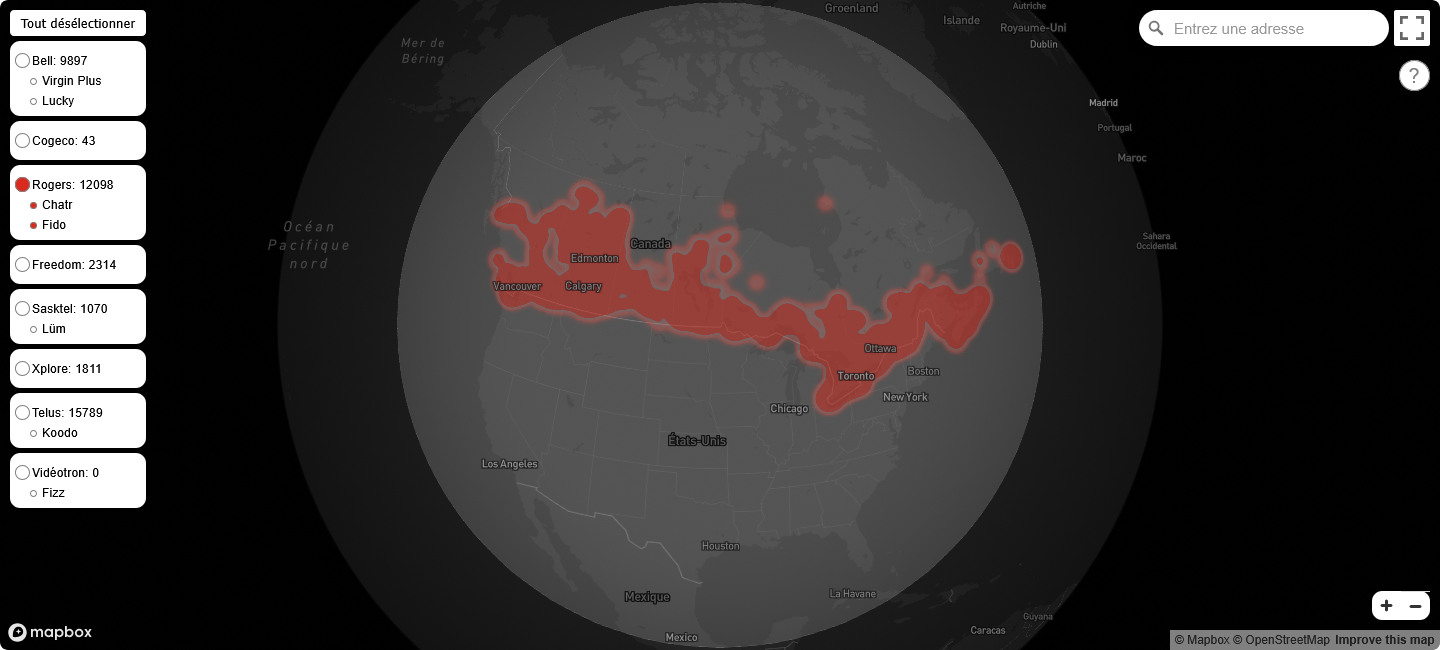
\includegraphics[width=0.85\textwidth]{figures/roger_networks.png}
\caption{Nodos Roger}
\label{fig:roger}
\vspace{0.15cm}
\begin{flushleft}
{\small \textbf{Nota.} Mapa que expresa la interconectividad de la red Rogers de 12098 puntos georreferenciados de cobertura de red en todo Canad\'{a}, de los cuales aproximadamente 380 se encuentran en la regi\'{o}n de Quebec, a diferencia de los 6600 que se encuentran en las ciudades m\'{a}s pobladas de Ontario (de las cuales incluyen Toronto y Ottawa). Elaboraci\'{o}n propia en base a datos de cobertura de red de Rogers obtenidos de PlanHub Canada.}
\end{flushleft}
\end{figure}

La estimaci\'on mediante M\'inimos Cuadrados Ponderados (WLS), que corrige la heterogeneidad asociada al tama\~no poblacional, revela una ca\'ida sustancial en la movilidad vinculada al consumo de bienes esenciales ($\beta = -38.5925$). Dicho hallazgo resulta compatible con mecanismos de amplificaci\'on asociados a estructuras altamente concentradas, en l\'inea con la Hip\'otesis Granular de \cite{gabaix2011granular} y los modelos de redes de \cite{acemoglu2012network, carvalho2014micro}, aunque el dise\~no emp\'irico no permite identificar directamente los canales espec\'ificos de transmisi\'on. Asimismo, las estimaciones del Estudio de Eventos muestran que la contracci\'on alcanza su m\'axima intensidad varios d\'ias despu\'es del \textit{shock} inicial. Este patr\'on puede interpretarse como compatible con mecanismos de propagaci\'on log\'istica y descoordinaci\'on temporal que prolongan los efectos m\'as all\'a de la interrupci\'on t\'ecnica original, potencialmente asociados a procesos de reposici\'on e intercambio de informaci\'on caracter\'isticos de cadenas de suministro operadas bajo esquemas \textit{Just-in-Time} (JIT) \citep{carvalho2021supply, barrot2016input}.

Mientras la literatura macrofinanciera cl\'asica se centra en v\'inculos patrimoniales o corridas de liquidez bancaria \citep{allen2000financial, hanson2011macroprudential, borio2011implementing}, la evidencia presentada indica que vulnerabilidades equivalentes emergen sin deterioro de balances institucionales. La econom\'ia contempor\'anea opera como una red multicapa o \textit{multiplex} \citep{buldyrev2010catastrophic, dedomenico2013mathematical, kivela2014multilayer}, donde perturbaciones en nodos de elevada centralidad pueden propagarse a trav\'es de distintos canales funcionales, en l\'inea con la literatura sobre fragilidad sist\'emica y riesgo cibern\'etico \citep{acemoglu2015systemic, golub20222fragilitysurvey, tian2023cybersecurity, panetta2025systemic}. En este entorno, la redundancia f\'isica (los cajeros autom\'aticos) pierde efectividad si la capa l\'ogica subyacente de conectividad colapsa de forma coordinada.

Esta din\'amica expone la fragilidad inherente a econom\'ias altamente digitalizadas. Conforme al an\'alisis de \citep{alvarez2009financial}, la innovaci\'on financiera optimiza la eficiencia operativa diaria al reducir la necesidad de mantener saldos precautorios de efectivo f\'isico. Sin embargo, en el l\'imite, los hogares minimizan sus m\'argenes de contingencia. El resultado es un \textit{trade-off} restrictivo entre eficiencia transaccional y robustez sist\'emica ante fallas de la infraestructura digital. A medida que los sistemas financieros avanzan hacia infraestructuras de pagos instant\'aneos, plataformas de dinero m\'ovil y potenciales esquemas de moneda digital de banco central (CBDC), la resiliencia de las redes de procesamiento de datos adquiere una importancia macroprudencial cr\'itica \citep{auer2020technology, katzbcra2022}. La estabilidad agregada pasa a depender de la continuidad operativa de la infraestructura digital que viabiliza el intercambio. 

En conjunto, la evidencia presentada sugiere que las infraestructuras digitales de pago constituyen un insumo esencial para el funcionamiento de las econom\'ias contempor\'aneas. El episodio de Rogers sugiere que perturbaciones originadas en capas tecnol\'ogicas aparentemente perif\'ericas pueden traducirse r\'apidamente en restricciones reales sobre el intercambio, propagarse a trav\'es de redes econ\'omicas interdependientes y generar efectos agregados significativos aun en ausencia de crisis financieras convencionales \citep{barabasi2016network, newman2010networks}.

La evidencia presentada sugiere que la resiliencia de estas infraestructuras podr\'ia desempe\~nar un papel cada vez m\'as relevante para la estabilidad macroecon\'omica en econom\'ias crecientemente digitalizadas. En consecuencia, las interrupciones de conectividad y procesamiento de pagos emergen como una dimensi\'on adicional del riesgo sist\'emico que merece una consideraci\'on m\'as expl\'icita dentro de los marcos anal\'iticos de estabilidad financiera y macroecon\'omica.

\newpage
\section{Cap\'itulo VIII: Conclusi\'on y Discusi\'on Integrada}
\label{chp:capitulo8}

\subsection{Recomendaciones Macroprudenciales y Agenda Futura}
\label{sec:8_1}

Los resultados de esta investigaci\'on sugieren que la estabilidad de los sistemas de pago contempor\'aneos depende no s\'olo de la solvencia de las instituciones financieras, sino tambi\'en de la resiliencia de las infraestructuras digitales que permiten la autorizaci\'on, transmisi\'on y liquidaci\'on de transacciones. En econom\'ias altamente digitalizadas, las redes de telecomunicaciones constituyen un insumo esencial para la circulaci\'on efectiva de la liquidez y, por lo tanto, deben ser consideradas dentro del per\'imetro de an\'alisis macroprudencial.

Desde esta perspectiva, una primera implicancia consiste en ampliar los ejercicios tradicionales de supervisi\'on y pruebas de estr\'es para incorporar vulnerabilidades asociadas a infraestructuras cr\'iticas de conectividad. La evidencia presentada muestra que interrupciones localizadas pueden propagarse m\'as all\'a de los l\'imites del sector tecnol\'ogico y generar efectos reales sobre el consumo, la movilidad y la coordinaci\'on econ\'omica agregada. En consecuencia, la evaluaci\'on de riesgos sist\'emicos deber\'ia incorporar expl\'icitamente la estructura de dependencias entre proveedores de telecomunicaciones, sistemas de compensaci\'on y plataformas de pago, siguiendo los desarrollos recientes sobre redes complejas e interdependientes.

Una segunda implicancia refiere al dise\~no de mecanismos de resiliencia. La ausencia de efectos mitigadores asociados a la densidad de cajeros autom\'aticos sugiere que la mera existencia de canales f\'isicos alternativos resulta insuficiente cuando \'estos dependen de la misma infraestructura l\'ogica subyacente. Este resultado abre interrogantes relevantes sobre el desarrollo de arquitecturas de pago con mayores niveles de redundancia operativa, incluyendo mecanismos de liquidaci\'on \textit{offline}, sistemas distribuidos de validaci\'on y futuras implementaciones de monedas digitales de banco central dise\~nadas bajo criterios de continuidad operativa.

Por \'ultimo, esta tesina invita a abrir una agenda de investigaci\'on orientada a modelar la infraestructura transaccional como una red multicapa donde interact\'uan sistemas de telecomunicaciones, plataformas de pago, cadenas log\'isticas y decisiones de los hogares. La incorporaci\'on expl\'icita de estas interdependencias permitir\'ia avanzar hacia una comprensi\'on m\'as precisa de los mecanismos mediante los cuales \textit{shocks} tecnol\'ogicos localizados pueden transformarse en perturbaciones macroecon\'omicas agregadas.

\subsection{Reflexi\'on Final}
\label{sec:8_2}

Esta tesina examin\'o los efectos econ\'omicos del apag\'on nacional de Rogers Communications ocurrido en Canad\'a el 8 de julio de 2022, utilizando la interrupci\'on simult\'anea de la infraestructura de telecomunicaciones y pagos como un experimento cuasi-natural para identificar el impacto de una falla tecnol\'ogica sobre la actividad econ\'omica real.

La evidencia obtenida permite concluir que la disrupci\'on produjo una contracci\'on significativa de la movilidad asociada al consumo de bienes esenciales, con una intensidad creciente seg\'un el grado de exposici\'on territorial a la red afectada. Los distintos ensayos de robustez, las pruebas placebo, los an\'alisis din\'amicos y los modelos de triple diferencia convergen en una misma interpretaci\'on: el mecanismo de transmisi\'on m\'as plausible oper\'o a trav\'es de una restricci\'on transaccional localizada en la infraestructura de pagos, m\'as que mediante \textit{shocks} clim\'aticos, alteraciones generalizadas de movilidad o respuestas conductuales homog\'eneas.

Estos resultados aportan evidencia emp\'irica consistente con los modelos de liquidaci\'on condicionada (\textit{Settlement-in-Advance}), mostrando que la capacidad efectiva de utilizar medios de pago digitales depende cr\'iticamente de la continuidad operativa de la infraestructura tecnol\'ogica que los sustenta. Cuando dicha infraestructura falla, la liquidez disponible deja de traducirse autom\'aticamente en capacidad de intercambio econ\'omico.

En t\'erminos m\'as amplios, la investigaci\'on sugiere que la digitalizaci\'on transforma la naturaleza del riesgo sist\'emico. A medida que la actividad econ\'omica depende crecientemente de redes de comunicaci\'on y validaci\'on electr\'onica, la estabilidad macroecon\'omica pasa a estar condicionada por factores tradicionalmente considerados externos al an\'alisis monetario y financiero. La experiencia canadiense muestra que una perturbaci\'on originada en la capa tecnol\'ogica puede propagarse r\'apidamente hacia la econom\'ia real, revelando que la resiliencia de los sistemas de pago constituye una dimensi\'on central de la estabilidad econ\'omica contempor\'anea.

En \'ultima instancia, el principal aporte de esta tesina consiste en documentar que la infraestructura digital de pagos no constituye un elemento auxiliar del sistema econ\'omico, sino una condici\'on necesaria para su funcionamiento cotidiano. Analizar esta dependencia resulta fundamental para dise\~nar marcos regulatorios capaces de enfrentar los desaf\'ios de una econom\'ia crecientemente digitalizada e interconectada.

\newpage
% =================================================
% BLOQUE DE ANEXOS Y AP\'eNDICES
% =================================================
\newpage
\pagenumbering{Roman}
\appendix
\addcontentsline{toc}{section}{Anexos}

\counterwithin{table}{section}
\counterwithin{figure}{section}
\counterwithin{equation}{section}

\newpage
\section{Anexo A: Formalizaci\'on Econom\'etrica e Inferencia Causal}
\label{anx:anexo_a}

La estrategia emp\'irica desarrollada en esta investigaci\'on pertenece a la tradici\'on de inferencia causal de forma reducida (\textit{reduced-form}), donde la identificaci\'on surge de una perturbaci\'on ex\'ogena observada y no de la estimaci\'on de un modelo estructural completo de comportamiento. En consecuencia, los par\'ametros obtenidos deben interpretarse como efectos causales promedio asociados al \textit{shock} de infraestructura estudiado, sin pretender recuperar de forma exhaustiva los mecanismos microecon\'omicos subyacentes que generan dicha respuesta agregada \citep{angrist2009mostly, cunningham2021causal, heckman1989choosing}.

\subsection{Evoluci\'on del Dise\~no Econom\'etrico}
\label{sec:A_1}

En esta secci\'on se expone el desarrollo algebraico formal y la justificaci\'on asint\'otica de la transici\'on desde los estimadores de l\'inea base agrupados hacia el modelo estructural m\'as exigente de Efectos Fijos Bidireccionales ponderados por masa demogr\'afica ($TWFE\text{-}WLS$). El punto de partida metodol\'ogico est\'a dictado por la especificaci\'on can\'onica lineal de Diferencias en Diferencias ($DiD$) bajo M\'inimos Cuadrados Ordinarios agrupados (\textit{Pooled OLS}):

\begin{equation}
    Y_{i,t} = \alpha + \beta_1 \left( Shock_t \times Exposure_i \right) + \beta_2 Shock_t + \beta_3 Exposure_i + \varepsilon_{i,t}
\end{equation}

Donde el par\'ametro $\beta_1$ opera como el estimador b\'asico del impacto del colapso de red condicionado al nivel continuo de penetraci\'on regional de Rogers. El supuesto de identificaci\'on ortogonal requiere que $\textit{$E$}[\varepsilon_{i,t} | Shock_t, Exposure_i] = 0$. Sin embargo, la literatura de evaluaci\'on de impacto advierte que la ausencia de controles para caracter\'isticas espaciales invariantes y shocks agregados correlacionados en el tiempo introduce un sesgo severo de variables omitidas que invalida la consistencia de $\hat{\beta}_1$ \citep{goodman2021difference, meyer1995natural}. Para purgar estas fuentes latentes de endogeneidad, el sistema se somete a una transformaci\'on intragrupo bidireccional, transitando hacia el modelo cl\'asico de Efectos Fijos de Dos V\'ias ($TWFE$):

\begin{equation}
    Y_{i,t} = \beta \left( Shock_t \times Exposure_i \right) + \alpha_i + \gamma_t + \varepsilon_{i,t}
\end{equation}

Los vectores de par\'ametros incidentes de secci\'on cruzada ($\alpha_i$) y serie de tiempo ($\gamma_t$) absorben las asimetr\'ias de intercepto por colinealidad perfecta, provocando la omisi\'on mec\'anica de los t\'erminos lineales simples presentes en la especificaci\'on agrupada. La identificaci\'on del par\'ametro estructural de inter\'es se define formalmente mediante la derivada parcial del valor esperado condicionado del sistema:

\begin{equation}
    \beta = \frac{\partial \textit{$E$}\left[ Y_{i,t} \mid \alpha_i, \gamma_t, Exposure_i, Shock_t \right]}{\partial \left( Shock_t \times Exposure_i \right)}
\end{equation}

Bajo los supuestos de fricci\'on nula de mercado, un shock puramente temporal e infraestructural deber\'ia disiparse de manera inmediata en el per\'iodo del evento ($t_0$). No obstante, la existencia de costos de men\'u, rigideces de liquidez transaccional e inatenci\'on racional sugiere patrones de hist\'eresis \citep{alvarez2009financial, sims2003implications}. Esto exige flexibilizar el supuesto est\'atico y mutar hacia un dise\~no din\'amico de \textit{Event Study} que distribuya los impactos diarios a lo largo de un horizonte m\'ovil compuesto por $q$ adelantos y $p$ rezagos temporales \citep{schmidheiny2019event}:

\begin{equation}
    Y_{i,t} = \alpha_i + \gamma_t + \sum_{\tau = -q}^{p} \beta_{\tau} D_{i,t}^{(\tau)} + \varepsilon_{i,t}
\end{equation}

Donde $D_{i,t}^{(\tau)} = (t - t_0 = \tau) \times Exposure_i$ identifica el regresor continuo del tratamiento indexado al d\'ia relativo $\tau$. Para garantizar la validez del dise\~no, se impone la restricci\'on param\'etrica de exclusi\'on sobre el per\'iodo inmediatamente anterior a la falla ($\beta_{-1} = 0$), consolidando la l\'ogica de comparabilidad contrafactual y permitiendo el testeo de tendencias paralelas bivariadas \citep{rambachan2023credible, baker2026difference, callaway2021difference}.

A pesar de las ventajas del modelo din\'amico, el sistema federal canadiense presenta una severa asimetr\'ia en el tama\~no de sus cl\'usteres provinciales, violando el supuesto can\'onico de perturbaciones homoced\'asticas e id\'enticamente distribuidas. De acuerdo con el marco te\'orico de la macro-granularidad econ\'omica \citep{gabaix2011granular}, las fluctuaciones de variables agregadas en muestras geogr\'aficas peque\~nas est\'an dominadas por choques granulares en nodos cr\'iticos (como Ontario), de modo que una estimaci\'on por M\'inimos Cuadrados Ordinarios asigna un peso desproporcionado a la varianza residual de provincias perif\'ericas con baja densidad transaccional \citep{moulton1990aggregate}. Para corregir este sesgo de escala y estabilizar la eficiencia del estimador, la estrategia de identificaci\'on incorpora un esquema de M\'inimos Cuadrados Ponderados ($WLS$) basado en el vector ex\'ogeno de masa demogr\'afica censal $w_i = Pop_i$ \citep{statscan2021pop}, cuyo criterio global de optimizaci\'on se define como:

\begin{equation}
    \min_{\beta_{\tau}} \sum_{i=1}^{N} \sum_{t=1}^{T} Pop_i \left( Y_{i,t} - \alpha_i - \gamma_t - \sum_{\tau = -q}^{p} \beta_{\tau} D_{i,t}^{(\tau)} \right)^2
\end{equation}

Expresado formalmente en notaci\'on matricial compacta, el estimador del perfil din\'amico del sistema se deriva como:

\begin{equation}
    \hat{\mathbf{\beta}}_{WLS} = \left( \mathbf{X}' \mathbf{W} \mathbf{X} \right)^{-1} \mathbf{X}' \mathbf{W} \mathbf{Y}
\end{equation}

Donde $\mathbf{X}$ denota la matriz de dise\~no que agrupa las interacciones continuas temporales junto al espacio nulo de los efectos fijos bidireccionales, $\mathbf{Y}$ representa el vector columna de respuesta de movilidad de consumo minorista, y $\mathbf{W}$ constituye la matriz de ponderaci\'on diagonal de tama\~no $(NT \times NT)$, parametrizada estrictamente por:

\begin{equation}
    \mathbf{W} = \text{diag}(w_1, w_2, \dots, w_N) \otimes \mathbf{I}_T
\end{equation}

Es imperativo formular una advertencia inferencial cr\'itica respecto al estimador puntual resultante. Dado que la matriz de pesos demogr\'aficos responde a criterios de agregaci\'on macroecon\'omica regional y no al rec\'iproco exacto de la varianza condicional latente de las perturbaciones ($\mathbf{W} \neq \mathbf{\Sigma}^{-1}$), la matriz de varianza-covarianza te\'orica del estimador no adopta la reducci\'on lineal est\'andar. Por el contrario, la estructura anal\'itica de los errores exige la instrumentaci\'on de un estimador de tipo s\'andwich robusto a cl\'usteres geogr\'aficos estructurado de la siguiente forma \citep{cameron2006robust, wooldridge2011econometric}:

\begin{equation}
    \mathbf{V}(\hat{\mathbf{\beta}}_{WLS}) = \left( \mathbf{X}' \mathbf{W} \mathbf{X} \right)^{-1} \left( \mathbf{X}' \mathbf{W} \mathbf{M}_C \mathbf{W} \mathbf{X} \right) \left( \mathbf{X}' \mathbf{W} \mathbf{X} \right)^{-1}
\end{equation}

Donde $\mathbf{M}_C$ representa la matriz block-diagonal de dispersi\'on clusterizada a nivel provincial, definida anal\'iticamente mediante la sumatoria del producto exterior de los vectores de residuos sectoriales:

\begin{equation}
    \mathbf{M}_C = \sum_{g=1}^{G} \mathbf{X}_g' \hat{\mathbf{u}}_g \hat{\mathbf{u}}_g' \mathbf{X}_g
\end{equation}

Donde $\hat{\mathbf{u}}_g$ constituye el vector de residuos estimado bajo el modelo ponderado para la provincia $g$. Esta formulaci\'on anal\'itica blinda la inferencia asint\'otica del modelo, garantizando que los errores est\'andar y los estad\'isticos t de la especificaci\'on $TWFE\text{-}WLS$ permanezcan invariantes y consistentes ante procesos arbitrarios de autocorrelaci\'on serial intraprovincial y heterocedasticidad cruzada de escala regional.

\subsection{Propiedades Din\'amicas y An\'alisis de Sensibilidad}
\label{sec:A_3}

Modelar la persistencia temporal de la fricci\'on exige extender la l\'ogica est\'atica hacia las especificaciones din\'amicas evaluadas en las rutinas computacionales. Con el prop\'osito de contrastar la presencia de rigideces estructurales y patrones de hist\'eresis en la velocidad de circulaci\'on, se generaliza el estimador base hacia una especificaci\'on de rezagos y adelantos flexibles (\textit{Event Study}) \citep{schmidheiny2019event} que adopta la estructura anal\'itica:
\begin{equation}
    Y_{i,t} = \alpha_i + \gamma_t + \sum_{k \neq -1} \beta_k \left( \text{Exposure}_i \times D_t^k \right) + \varepsilon_{i,t}
    \label{eq:event_study}
\end{equation}

Donde las variables indicadoras de tiempo relativo se definen formalmente mediante la funci\'on condicional:

\begin{equation}
    D_t^k = \textit{$I$}(\text{rel\_time} = k)
\end{equation}

Asumiendo al per\'iodo $k = -1$ como la categor\'ia base de referencia excluida para asegurar la identificaci\'on param\'etrica del sistema \citep{angrist2009mostly}. Bajo este dise\~no, el vector de coeficientes $\beta_k$ captura el efecto causal diferencial del shock para cada d\'ia relativo al hito del colapso de red.

Para evaluar de forma rigurosa la vulnerabilidad de estos estimadores din\'amicos ante posibles violaciones al supuesto fundamental de tendencias paralelas, el marco metodol\'ogico incorpora una aproximaci\'on simplificada de honestidad param\'etrica inspirada en la l\'ogica de l\'imites del peor escenario (\textit{Worst-Case Bounds}). El procedimiento no implementa el algoritmo de optimizaci\'on convexo formal de Rambachan-Roth, sino que instrumenta una heur\'istica lineal directa sobre el espectro de coeficientes hist\'oricos previos al evento ($k < 0$). Se computa inicialmente la m\'axima distorsi\'on absoluta observada en la fase de pre-trend mediante:

\begin{equation}
    \Delta = \max_{k < 0} \left| \hat{\beta}_k \right|
\end{equation}

Asumiendo que este sesgo m\'aximo latente se proyecta de forma aditiva sobre el d\'ia del evento ex\'ogeno ($T_0$), se define el l\'imite del peor escenario posible para el par\'ametro de impacto como:

\begin{equation}
    \beta_0^{worst} = \hat{\beta}_0 + \Delta
\end{equation}

Mec\'anicamente, la introducci\'on de $\Delta$ requiere una discusi\'on asint\'otica formal. Dado que cada $\hat{\beta}_k$ para $k < 0$ constituye una variable aleatoria normalizada tal que $\hat{\beta}_k \sim \mathcal{N}(\beta_k, \sigma_k^2)$, el estad\'istico extremal $\Delta$ opera bajo las propiedades de la distribuci\'on del m\'aximo absoluto de un vector multivariado. Bajo la hip\'otesis nula de tendencias paralelas estrictas ($\beta_k = 0, \forall k < 0$), el valor esperado de $\Delta$ es estrictamente creciente respecto al cardinal del soporte temporal de pre-evento, producto de la acumulaci\'on del error Tipo I en escenarios de inferencia s\'incrona \citep{rambachan2023credible}. 

Para neutralizar el sesgo de selecci\'on del m\'aximo hist\'orico o \textit{winner's curse} computacional, la evaluaci\'on no asume a $\Delta$ como un estimador puntual insesgado de la tendencia, sino como una funci\'on de penalizaci\'on acotada y maximal. Esta estrategia metodol\'ogica se alinea con la filosof\'ia de control de tasas de falso descubrimiento (\textit{False Discovery Rate}) bajo dependencias arbitrarias \citep{benjamini1995}, garantizando que la cota de tolerancia impuesta al estimador de impacto primario absorba de manera conservadora los extremos de la distribuci\'on de ruido muestral.

Finalmente, la robustez y la tolerancia del modelo frente a la volatilidad estacional subyacente de la serie se eval\'uan de forma estandarizada a trav\'es de la ratio heur\'istica de persistencia se\~nal/ruido ($R$), especificada como:

\begin{equation}
    R = \frac{\left| \hat{\beta}_0 \right|}{\Delta}
\end{equation}

Esta m\'etrica condensa la vulnerabilidad de la identificaci\'on estructural, donde un valor cr\'itico de $R < 1$ explicita matem\'aticamente la necesidad de aislar el an\'alisis mediante la contracci\'on controlada del soporte temporal (\textit{Bandwidth Sensitivity}) \citep{baker2026difference}, aislando el impacto real de las perturbaciones macro-ambientales de fondo.

\subsection{Inferencia No Param\'etrica y Placebos no Geogr\'aficos}
\label{sec:A_6}

Debido a la escasez de cl\'usteres geogr\'aficos independientes ($N=9$), las aproximaciones asint\'oticas de los errores est\'andar tradicionales tienden a sesgarse hacia abajo, incrementando la probabilidad de cometer un error de Tipo I (falso positivo) \citep{cameron2006robust}. Cuando el n\'umero de cl\'usteres $G \to \infty$, los teoremas del l\'imite central garantizan la consistencia del estimador de s\'andwich corporativo; sin embargo, un soporte de apenas nueve provincias canadienses representa un escenario cr\'itico de \textit{few clusters} que invalida la inferencia tradicional. Para corregir esta distorsi\'on e instrumentar un esquema de inferencia exacto en muestras peque\~nas, se adopta un algoritmo manual de \textit{Wild Cluster Bootstrap} ($t$-WCB) bajo la hip\'otesis nula restringida, potenciado algebraicamente por la descomposici\'on de Frisch-Waugh-Lovell (FWL).
El teorema de Frisch-Waugh-Lovell establece que el estimador de efectos fijos de dos v\'ias ($\hat{\beta}_{TWFE}$) puede expresarse formalmente en funci\'on de los vectores transformados por el operador de proyecci\'on ortogonal:

\begin{equation}
    \hat{\beta}_{TWFE} = \hat{\beta} \left( \mathbf{M}_{\mathbf{F}}\mathbf{Y}, \mathbf{M}_{\mathbf{F}}\mathbf{X} \right)
\end{equation}

Donde $\mathbf{M}_{\mathbf{F}} = \mathbf{I} - \mathbf{P}_{\mathbf{F}}$ constituye la matriz de aniquilaci\'on idempotente y sim\'etrica que proyecta los datos sobre el espacio ortogonal de los efectos fijos bidireccionales. En las rutinas computacionales del sistema, esta operaci\'on se ejecuta mediante un doble centrado (\textit{double demeaning}) aditivo sobre el panel:

\begin{equation}
    \tilde{Y}_{i,t} = Y_{i,t} - \bar{Y}_i - \bar{Y}_t + \bar{Y}
\end{equation}
\begin{equation}
    \tilde{X}_{i,t} = X_{i,t} - \bar{X}_i - \bar{X}_t + \bar{X}
\end{equation}

Donde $X_{i,t} = \text{Shock}_t \times \text{Exposure}_i$ representa el regresor continuo de intensidad del tratamiento. El modelo residualizado colapsa as\'i en la especificaci\'on lineal can\'onica:

\begin{equation}
    \tilde{Y}_{i,t} = \beta \tilde{X}_{i,t} + u_{i,t}
    \label{eq:fwl_residual}
\end{equation}

La incorporaci\'on del paso FWL resulta metodol\'ogicamente fundamental para la viabilidad econ\'omica del bootstrap. Al parcializar los interceptos espaciales y temporales ex-ante, el algoritmo obvia la necesidad estr\'ategica de reestimar el vector completo de par\'ametros incidentes ($\alpha_i, \gamma_t$) en cada una de las iteraciones del bucle de simulaci\'on, reduciendo exponencialmente el costo y la alta carga computacional del remuestreo corporativo.

Sobre este modelo residualizado e id\'entico al sistema original, se impone r\'igidamente la hip\'otesis nula restringida $H_0: \beta = 0$. A diferencia de los m\'etodos de remuestreo de pares tradicionales que extraen observaciones directas $(y_i, x_i)$ alterando la estructura de las secciones cruzadas, el Wild Bootstrap perturba los residuos calculados bajo la nula a nivel de cl\'uster provincial $g$. El vector de pseudo-residuos bootstrap se define mediante la operaci\'on:

\begin{equation}
    u_{i,t}^{*(b)} = w_g^{(b)} \hat{u}_{i,t} \quad \forall \quad i,t \in g
\end{equation}

Donde el ponderador escalar aleatorio $w_g^{(b)}$ se extrae de la distribuci\'on de Webb de seis puntos \citep{mackinnon2020randomization}:

\begin{equation}
    w_g \in \left\{ -\sqrt{\frac{3}{2}}, -1, -\sqrt{\frac{1}{2}}, \sqrt{\frac{1}{2}}, 1, \sqrt{\frac{3}{2}} \right\}
\end{equation}

La elecci\'on del esquema de \citep{webb2014reworking} con una probabilidad uniforme de ocurrencia ($p = 1/6$) responde a propiedades asint\'oticas estrictas de momentos especificadas para estructuras con cl\'usteres severamente restringidos ($G < 10$), cumpliendo con:

\begin{equation}
    \textit{$E$}(w_g) = 0, \quad \textit{$E$}(w_g^2) = 1, \quad \textit{$E$}(w_g^4) = 3
\end{equation}

Dado que el peso sim\'etrico se mantiene constante para todas las observaciones temporales pertenecientes al mismo cl\'uster geogr\'afico, se preserva la estructura de autocorrelaci\'on intracl\'uster latente en el panel. Al imponerse la restricci\'on param\'etrica de la hip\'otesis nula, la variable de respuesta sint\'etica para cada r\'eplica de la simulaci\'on se reduce exclusivamente a la perturbaci\'on residual:

\begin{equation}
    Y_{i,t}^{*(b)} = w_g^{(b)} \hat{u}_{i,t}
\end{equation}

Posteriormente, el algoritmo ejecuta la reestimaci\'on recursiva a lo largo de $B = 999$ r\'eplicas independientes de Monte Carlo sobre la especificaci\'on de Frisch-Waugh-Lovell de fondo:

\begin{equation}
    Y_{i,t}^{*(b)} = \beta^{*(b)} \tilde{X}_{i,t} + \varepsilon_{i,t}^{*(b)}
\end{equation}

Para cada iteraci\'on $b$, se almacena el coeficiente transformado y se construye el estad\'istico t bootstrap estandarizado correspondiente:

\begin{equation}
    t^{*(b)} = \frac{\hat{\beta}^{*(b)}}{\text{SE}(\hat{\beta}^{*(b)})}
\end{equation}

El p-valor robusto final del estimador bootstrap ($p_{WCB}$) se calcula determinando la proporci\'on emp\'irica de estad\'isticos simulados bajo la nula que exceden en valor absoluto al estad\'istico t observado en la muestra real ($t_{obs}$):

\begin{equation}
    p_{WCB} = \frac{1}{B} \sum_{b=1}^{B} \textit{$I$} \left( \left| t_b^* \right| \ge \left| t_{obs} \right| \right)
    \label{eq:p_wcb_final}
\end{equation}

Es necesario advertir una restricci\'on inferencial de este enfoque en muestras balanceadas geogr\'aficamente concentradas. Debido a que el sistema federal canadiense limita el soporte de cl\'usteres a las fronteras provinciales ($N=9$), la implementaci\'on del algoritmo $t$-WCB bajo la distribuci\'on de Webb opera de forma estrictamente conservadora. Esta restricci\'on param\'etrica incrementa la varianza muestral simulada, empujando los p-valores hacia la no significancia asint\'otica en los contrastes bivariados m\'as exigentes \citep{mackinnon2017wild, roodman2019fast}.

El dise\~no emp\'irico se complementa mediante pruebas de permutaci\'on exacta basadas en el enfoque de Fisher utilizando $B = 1000$ iteraciones Monte Carlo \citep{fisher1966design, young2022consistency}, estructuradas bajo dos dimensiones independientes de aleatorizaci\'on. La primera de ellas eval\'ua la dimensi\'on de \textit{Fisher Espacial}, donde en cada iteraci\'on $b$ se permutan aleatoria y uniformemente los niveles de exposici\'on entre las secciones cruzadas provinciales:

\begin{equation}
    \text{Exposure}_i^{(b)} = \text{Permutaci\'on}(\text{Exposure}_i)
\end{equation}

Estimando subsecuentemente el modelo de efectos fijos expandido:

\begin{equation}
    Y_{i,t} = \beta_b (\text{Shock}_t \times \text{Exposure}_i^{(b)}) + \alpha_i + \gamma_t + \varepsilon_{i,t}
\end{equation}

Cuyo p-valor exacto de aleatorizaci\'on se define como:

\begin{equation}
    p_{spatial} = \frac{1}{B} \sum_{b=1}^{B} \textit{$I$} \left( \left| \beta_b \right| \ge \left| \hat{\beta} \right| \right)
\end{equation}

La segunda dimensi\'on incorpora el test de \textit{Fisher Temporal}, aislando el canal de transmisi\'on cronol\'ogico mediante el reemplazo de la fecha real del evento por una jornada ordinaria placebo ex-ante ($\text{FakeShock}_t^{(b)} = \mathbb{I}(t = f_b)$), lo cual redefine el regresor de interacci\'on de la secci\'on cruzada como $\text{FakeX}_{i,t}^{(b)} = \text{FakeShock}_t^{(b)} \times \text{Exposure}_i$. Tras estimar la especificaci\'on contrafactual:

\begin{equation}
    Y_{i,t} = \beta_b \text{FakeX}_{i,t}^{(b)} + \alpha_i + \gamma_t + \varepsilon_{i,t}
\end{equation}

Se computa el p-valor temporal mediante la misma funci\'on indicadora de masa de probabilidad:

\begin{equation}
    p_{temp} = \frac{1}{B} \sum_{b=1}^{B} \textit{$I$} \left( \left| \beta_b \right| \ge \left| \hat{\beta} \right| \right)
\end{equation}

En una red macroecon\'omica concentrada ($N=9$), las pruebas de permutaci\'on espacial pueden alterar de forma mec\'anica el p-valor. Al permutar la matriz de tratamiento y asignarle de manera aleatoria la masa cr\'itica de Ontario a una provincia perif\'erica, se generan distribuciones nulas sint\'eticas de alta volatilidad residual debido al car\'acter no id\'enticamente distribuido de los shocks granulares en muestras geogr\'aficamente asim\'etricas \citep{ferman2019inference, mackinnon2020randomization}.

Espec\'ificamente, dado que el estimador se parametriza mediante m\'inimos cuadrados ponderados utilizando la masa poblacional como ponderador matricial, la reasignaci\'on pseudo-aleatoria del vector de intensidades de tratamiento quiebra la homogeneidad de los residuos transformados. Al adscribir la ponderaci\'on extrema de Ontario a un vector de exposici\'on ex\'ogeno de otra provincia con menor escala muestral, la matriz de varianzas y covarianzas residuales experimenta un sesgo de esfericidad inducido mec\'anicamente, incrementando de forma artificial la varianza de los coeficientes de placebo en la distribuci\'on contrafactual de Fisher \citep{fisher1966design}.

\subsection{Selectividad Transaccional y Falsabilidad Multivariada}
\label{sec:A_5}

Para garantizar la validez del enfoque de falsabilidad multi-outcome y corregir las distorsiones inducidas por el contraste simult\'aneo de m\'ultiples hip\'otesis, el marco emp\'irico incorpora el procedimiento de ajuste de Benjamini-Hochberg \citep{benjamini1995}. Dado un conjunto de $m$ p-valores ordenados de forma ascendente:
\begin{equation}
    p_{(1)} \le p_{(2)} \le \cdots \le p_{(m)}
\end{equation}

La correcci\'on inicial de falsos descubrimientos se aplica mediante la funci\'on condicional:

\begin{equation}
    p^{BH}_{(i)} = \min \left( 1, \frac{m}{i} p_{(i)} \right)
\end{equation}

Garantizando la consistencia del ordenamiento mediante la imposici\'on estricta de monoton\'ia:

\begin{equation}
    p^{adj}_{(i)} = \min_{j \ge i} p^{BH}_{(j)}
\end{equation}

Este algoritmo permite controlar de forma robusta la Tasa de Falso Descubrimiento ($FDR$), definida anal\'iticamente como la esperanza matem\'atica de la proporci\'on de falsos positivos sobre el total de rechazos:

\begin{equation}
    FDR = \textit{$E$} \left[ \frac{V}{R} \right]
\end{equation}

Donde $V$ denota el n\'umero de hip\'otesis nulas err\'oneamente rechazadas (falsos positivos) y $R$ constituye la cantidad total de rechazos registrados en el sistema.

Una vez calibrada la significancia conjunta, se testea emp\'iricamente la hip\'otesis de selectividad transaccional ---seg\'un la cual el shock de conectividad minorista interrumpe los canales de liquidaci\'on condicionada sin deprimir de forma sim\'etrica los desplazamientos humanos agregados--- mediante la estimaci\'on de un modelo de Triples Diferencias ($DDD$) \citep{gruber1994incidence, meyer1995natural}. Para ello, se construye un panel apilado estructurado en la dimensi\'on $j$, donde $j=1$ identifica de forma exclusiva al vector de movilidad comercial minorista e inelasticidad del consumo ($Grocery$), mientras que $j=0$ indexa secuencialmente a los destinos de control placebo ($Residential$, $Parks$ o $Transit$). Esta estrategia de identificaci\'on permite aislar los sesgos de confusi\'on contempor\'aneos y las tendencias macro-ambientales comunes que afectan la movilidad global \citep{wooldridge2011econometric}, proveyendo una m\'etrica m\'as limpia de los canales de transmisi\'on transaccionales \citep{chetty2009sufficient}. Se define formalmente la variable indicadora de selectividad como:

\begin{equation}
    \text{Inelasticity}_j = \begin{cases} 1 & \text{si } j = \text{Grocery} \\ 0 & \text{si } j = \text{Placebo} \end{cases}
\end{equation}

La especificaci\'on econom\'etrica expandida para el panel apilado se desglosa en varias l\'ineas para resguardar los m\'argenes del documento:

\begin{equation}
\begin{aligned}
    Y_{i,j,t} = & \beta_1 \left( \text{Shock}_t \times \text{Exposure}_i \times \text{Inelasticity}_j \right) + \beta_2 \left( \text{Shock}_t \times \text{Inelasticity}_j \right) \\
    & + \beta_3 \left( \text{Shock}_t \times \text{Exposure}_i \right) + \beta_4 \left( \text{Exposure}_i \times \text{Inelasticity}_j \right) \\
    & + \beta_5 \text{Shock}_t + \beta_6 \text{Inelasticity}_j + \alpha_i + \gamma_t + \varepsilon_{i,j,t}
\end{aligned}
\label{eq:triple_interaction}
\end{equation}

Donde los par\'ametros estimados corresponden exactamente a los componentes lineales y cruzados del sistema, mapeando de forma directa las interacciones de control ($\beta_1 = \text{Shock\_x\_Exp\_x\_Inel}$, $\beta_2 = \text{Shock\_x\_Inel}$, $\beta_3 = \text{Shock\_x\_Exp}$, $\beta_4 = \text{Exp\_x\_Inel}$). Los coeficientes directos $\beta_5$ ($\text{Shock}_t$) y $\beta_6$ ($\text{Inelasticity}_j$) controlan las desviaciones de intercepto del d\'ia del evento y las asimetr\'ias estructurales promedio entre categor\'ias de consumo, mientras que los efectos fijos bidireccionales de provincia ($\alpha_i$) y d\'ia ($\gamma_t$) absorben las heterogeneidades espaciales y temporales no observables del panel. El par\'ametro de inter\'es cr\'itico est\'a determinado por el estimador de triple interacci\'on $\beta_1$, dado que su magnitud e identificaci\'on a\'islan formalmente si el colapso infraestructural golpea con mayor intensidad y significancia relativas a la movilidad comercial transaccional que a las dimensiones ortogonales y conductuales utilizadas como placebo \citep{angrist2009mostly}.

\newpage
\section{Anexo B: Microfundamentos Matem\'aticos del Marco SIA/TIL}
\label{anx:anexo_b}

\subsection{Advertencia Epistemol\'ogica y Naturaleza de la Formalizaci\'on}\label{sec:B_1}

El marco anal\'itico desarrollado en este anexo no constituye un modelo estructural plenamente estimado en el sentido de \citet{heckman1989choosing}, ni pretende identificar par\'ametros profundos de preferencia o de b\'usqueda de forma un\'ivoca. Dado que la estrategia econom\'etrica principal es de naturaleza reducida y basada en un experimento natural, las ecuaciones din\'amicas, las funciones de emparejamiento y la optimizaci\'on intertemporal mediante Hamiltoniano aqu\'i expuestas no deben interpretarse como objetos identificados r\'igidamente por los datos.

Por el contrario, el andamiaje formal SIA/TIL funciona estrictamente como una formalizaci\'on conceptual consistente en forma reducida. Su objetivo es organizar de manera coherente y rigurosa las analog\'ias anal\'iticas y los mecanismos tecnolog\'icos plausibles que resultan compatibles con los patrones emp\'iricos estimados. En este sentido, la utilizaci\'on de funciones de emparejamiento inspiradas en la tradici\'on Diamond-Mortensen-Pissarides (DMP) y la optimizaci\'on de horizontes din\'amicos mediante Hamiltonianos continuos no asumen un comportamiento estructural de largo plazo, sino que operan como herramientas matem\'aticas estilizadas para capturar de forma compacta la direcci\'on de la cu\~na transaccional instant\'anea ($\mu_t$), la par\'alisis informacional de alta frecuencia y las din\'amicas de compensaci\'on intertemporal (\textit{catch-up}) observadas tras el restablecimiento f\'isico de la red.

Bajo este enfoque, el aparato matem\'atico ilustra la consistencia din\'amica del canal infraestructural puro, proponiendo una racionalizaci\'on donde la infraestructura de pagos no opera como un velo tecnol\'ogico neutral, sino como una restricci\'on operacional continua y de corto plazo en una red m\'ultiplex interdependiente.

Formalmente, la capacidad agregada de liquidaci\'on se define como:

\begin{equation}
\label{eq:Nt}
N_t = G(E_t, T_t, C_t, B_t, A_t)
\end{equation}
donde:
\begin{itemize}
    \item $E_t$ representa la continuidad del suministro el\'ectrico;
    \item $T_t$ el estado operativo de las redes de telecomunicaciones;
    \item $C_t$ la capacidad de procesamiento computacional;
    \item $B_t$ la disponibilidad de la infraestructura bancaria y de compensaci\'on;
    \item $A_t$ la capacidad operativa de los mecanismos alternativos de liquidaci\'on.
\end{itemize}

Formalmente, el operador funcional $\mathcal{G}(\cdot)$ adopta la estructura de un mapeo de proporciones fijas del tipo Leontief generalizado, definido sobre variables continuas de estado tal que 

\begin{equation}
G(\cdot) = \min\{E_t, T_t, C_t, B_t, A_t\}
\end{equation}

donde las capas cr\'iticas se normalizan en el intervalo $[0,1]$. 

Esta especificaci\'on microfundamenta matem\'aticamente por qu\'e una degradaci\'on granular en el ruteo o en la densidad de enlaces telem\'aticos activos ($T_t \in [0,1]$) arrastra de forma lineal y restrictiva a la capacidad agregada de liquidaci\'on del sistema ($N_t = T_t$), provocando que las perturbaciones sectoriales parciales en los nodos de telecomunicaciones se amplifiquen end\'ogenamente sin necesidad de un colapso f\'isico anal\'ogico absoluto, generando efectos y umbrales no lineales consistentes con la literatura de riesgo sist\'emico granular y redes complejas \citep{acemoglu2012network, panetta2025systemic}. 

Es imperativo destacar que esta especificaci\'on Leontief debe interpretarse estrictamente como una representaci\'on estilizada de cuellos de botella cr\'iticos en infraestructura interdependiente y no como una descripci\'on literal del grado emp\'irico de sustituibilidad entre capas en condiciones ordinarias de mercado \citep{auer2020technology, kahn2009pay}.

\subsection{Evoluci\'on y Transici\'on de Cadenas de Markov (DTMC)}
\label{sec:B_2}

Dado que la din\'amica transaccional de alta frecuencia exhibe una trayectoria de transici\'on fluida condicionada por la disponibilidad de la infraestructura l\'ogica, resulta conveniente utilizar una representaci\'on din\'amica en tiempo discreto. 

Para unificar esta secci\'on con el andamiaje general de la tesis, se establece un v\'inculo directo entre la capacidad global de liquidaci\'on del sistema de la ecuaci\'on \ref{eq:Nt} y el comportamiento estoc\'astico de los agentes. Espec\'ificamente, el nivel operativo y de capilaridad l\'ogica de la capa de telecomunicaciones ($T_t \in [0,1]$) determina de forma un\'ivoca la realizaci\'on del indicador continuo de conectividad macroecon\'omica del panel, tal que $\Omega_t = T_t$, donde $\Omega_t \in [0,1]$ indexa la proporci\'on de enlaces activos y protocolos BGP operativos en la malla. 

Las Cadenas de Markov de Tiempo Discreto (DTMC) y los modelos de b\'usqueda derivados de la tradici\'on neocl\'asica de fricciones del mercado ofrecen una aproximaci\'on \'util para representar estas transiciones graduales y efectos umbral de desborde inducidos por la degradaci\'on de la infraestructura de red \citep{acemoglu2012network, sargent2022economic}.

El mercado se compone por $N_{\text{D}}$ hogares (demandantes) y $N_{\text{S}}$ comercios (oferentes). En cada instante discreto $t$, los agentes pueden transitar entre los siguientes estados estilizados de liquidez:

\begin{itemize}
    \item $A^{\text{E}}$ (Equilibrio Transaccional Digital): Consumidores y comercios operando bajo condiciones de acceso regular a la infraestructura digital de pagos.
    \item $A^{\text{B}}$ (Estado de Amortiguaci\'on o \textit{Buffer stage}): Agentes que absorben la perturbaci\'on parcial mediante reservas f\'isicas o mecanismos de liquidaci\'on contingentes. Se divide en $A_{\text{D}}^{\text{B}}$ para hogares utilizando efectivo precautorio y $A_{\text{S}}^{\text{B}}$ para comercios operando con inventarios f\'isicos fuera de sistemas integrados.
    \item $A^{\text{R}}$ (Estado Restringido o \textit{Restricted stage}): Situaci\'on donde las restricciones operativas de la Capa TIL se vuelven de forma discreta vinculantes debido a la congesti\'on de la red, anulando la capacidad transaccional. Se divide en $A_{\text{D}}^{\text{R}}$ para consumidores que enfrentan costos de b\'usqueda o colapso de sus canales de liquidaci\'on, y $A_{\text{S}}^{\text{R}}$ para comercios afectados por la par\'alisis log\'istica.
    \item $A^{\text{C}}$ (Fase de Compensaci\'on Intertemporal o \textit{Catch-up stage}): Etapa posterior a la normalizaci\'on de la red donde parte del consumo postergado y del reabastecimiento log\'istico tiende a canalizarse gradualmente.
\end{itemize}

Para representar la din\'amica de frecuencia alta asociada al shock, el modelo adopta ecuaciones en diferencias de primer orden en tiempo discreto. Flexibilizando la rigidez binaria, las probabilidades de transici\'on entre estados se parametrizan de forma continua en funci\'on del grado de capilaridad remanente de la red ($\Omega_t$). La evoluci\'on din\'amica de la demanda agregada se aproxima mediante el siguiente sistema acoplado estable y conservativo:

\begin{equation}
    A^{\text{E}}_{\text{D}, t+1} = \Omega_t A^{\text{E}}_{\text{D}, t} + \delta_{\text{D}} A^{\text{C}}_{\text{D}, t}
    \label{eq:markov_demand_1}
\end{equation}

\begin{equation}
    A^{\text{B}}_{\text{D}, t+1} = (1 - \Omega_t) A^{\text{E}}_{\text{D}, t} + (1 - \alpha_{\text{D}} \Omega_t) A^{\text{B}}_{\text{D}, t}
    \label{eq:markov_demand_2}
\end{equation}

\begin{equation}
    A^{\text{R}}_{\text{D}, t+1} = A^{\text{R}}_{\text{D}, t} + \alpha_{\text{D}} \Omega_t A^{\text{B}}_{\text{D}, t} - \Omega_t \gamma_{\text{D},t} A^{\text{R}}_{\text{D}, t}
    \label{eq:markov_demand_3}
\end{equation}

\begin{equation}
    A^{\text{C}}_{\text{D}, t+1} = (1 - \delta_{\text{D}}) A^{\text{C}}_{\text{D}, t} + \Omega_t \gamma_{\text{D},t} A^{\text{R}}_{\text{D}, t}
    \label{eq:markov_demand_4}
\end{equation}

De forma sim\'etrica, el comportamiento transicional de la oferta minorista y corporativa se modela en espejo a partir de las restricciones f\'isicas de coordinaci\'on impuestas por la Capa TIL, delimitando la din\'amica de las firmas mediante el sistema din\'amico paralelo:

\begin{equation}
    A^{\text{E}}_{\text{S}, t+1} = \Omega_t A^{\text{E}}_{\text{S}, t} + \delta_{\text{S}} A^{\text{C}}_{\text{S}, t}
    \label{eq:markov_supply_1}
\end{equation}

\begin{equation}
    A^{\text{B}}_{\text{S}, t+1} = (1 - \Omega_t) A^{\text{E}}_{\text{S}, t} + (1 - \alpha_{\text{S}} \Omega_t) A^{\text{B}}_{\text{S}, t}
    \label{eq:markov_supply_2}
\end{equation}

\begin{equation}
    A^{\text{R}}_{\text{S}, t+1} = A^{\text{R}}_{\text{S}, t} + \alpha_{\text{S}} \Omega_t A^{\text{B}}_{\text{S}, t} - \Omega_t \gamma_{\text{S},t} A^{\text{R}}_{\text{S}, t}
    \label{eq:markov_supply_3}
\end{equation}

\begin{equation}
    A^{\text{C}}_{\text{S}, t+1} = (1 - \delta_{\text{S}}) A^{\text{C}}_{\text{S}, t} + \Omega_t \gamma_{\text{S},t} A^{\text{R}}_{\text{S}, t}
    \label{eq:markov_supply_4}
\end{equation}

La degradaci\'on de la infraestructura ($\Omega_t < 1$) gatilla una desviaci\'on proporcional de los flujos desde el equilibrio hacia los estados de amortiguaci\'on, capturando anal\'iticamente el impacto del racionamiento transaccional y la fragmentaci\'on topol\'ogica de la red. La evoluci\'on temporal del sistema se encuentra regulada por los par\'ametros cr\'iticos de transici\'on discriminados por canales ($\gamma_{\text{D},t}, \gamma_{\text{S},t}$), que representan las tasas de absorci\'on y normalizaci\'on de la demanda y oferta restringidas ponderadas por la velocidad de reconexi\'on de los enlaces l\'ogicos ($\Omega_t \gamma_{\text{D},t}, \Omega_t \gamma_{\text{S},t}$), operando como el puente din\'amico de reacomodamiento intertemporal; y los par\'ametros ($\delta_{\text{D}}, \delta_{\text{S}}$), que denotan las tasas de disipaci\'on o vaciado de las fases de compensaci\'on ($A^{\text{C}}$). 

A nivel probabil\'istico, la inclusi\'on de los par\'ametros $\delta_j > 0$ resulta indispensable para asegurar la ergodicidad y la estabilidad de largo plazo del sistema. De omitirse este flujo de vaciado, el estado de compensaci\'on intertemporal ($A^{\text{C}}$) mutar\'ia hacia un estado absorbente, provocando que toda la masa transaccional de la econom\'ia quedara confinada en dicho vector para $t \to \infty$ y destruyendo la naturaleza c\'iclica del intercambio. Al forzar el retorno de los agentes hacia el equilibrio base ($A^{\text{E}}$), se garantiza que la matriz de transici\'on sea irreducible y aperi\'odica (asumiendo $\Omega_t > 0$), confiriendo al sistema din\'amico una distribuci\'on estacionaria \'unica de r\'egimen permanente.

El modelo permite velocidades diferenciadas de vaciado de los inventarios monetarios contingentes entre hogares y comercios. Si se asume de manera consistente con los patrones observados que $\alpha_{\text{D}} > \alpha_{\text{S}}$, se refleja anal\'iticamente que los saldos precautorios de efectivo de los hogares se contraen m\'as r\'apidamente que las reservas f\'isicas de las firmas. Mientras los consumidores agotan con celeridad la liquidez manual disponible ante la p\'erdida de conexi\'on, los inventarios comerciales f\'isicos exhiben una menor velocidad de drenaje. No obstante, al encontrarse paralizada la telemetr\'ia y el software de clearing B2B de la Capa TIL, el desabastecimiento f\'isico eventual de las firmas es compatible con el hecho de que los mayores efectos contractivos netos estimados aparezcan con rezago temporal en las ventanas de horizontes intermedios del panel \citep{carvalho2021supply}.

Para verificar la consistencia estructural de este formalismo de Markov, resulta imperativo examinar anal\'iticamente el comportamiento de los sistemas compartimentales ante los dos escenarios extremos del espacio de fases del indicador de capilaridad $\Omega_t$:

\begin{enumerate}
    \item \textbf{Escenario de Colapso e Interrupci\'on Total ($\Omega_t = 0$):} Ante la par\'alisis absoluta de la red, las ecuaciones de movimiento de la demanda y de la oferta se reducen estrictamente a:
    \begin{align}
        A^{\text{E}}_{j, t+1} &= \delta_j A^{\text{C}}_{j, t} \\
        A^{\text{B}}_{j, t+1} &= A^{\text{E}}_{j, t} + A^{\text{B}}_{j, t} \\
        A^{\text{R}}_{j, t+1} &= A^{\text{R}}_{j, t} \\
        A^{\text{C}}_{j, t+1} &= (1 - \delta_j) A^{\text{C}}_{j, t}
    \end{align}
    Bajo este l\'imite topol\'ogico, se anula la capacidad de iniciar transacciones ordinarias en el equilibrio, provocando que todo el flujo planeado del d\'ia ($A^{\text{E}}_t$) choque contra la barrera tecnol\'ogica e incremente de forma herm\'etica la masa de transacciones bloqueadas en el buffer ($A^{\text{B}}$). Simult\'aneamente, los canales log\'isticos y de liquidaci\'on en la cola del clearing financiero se congelan instant\'aneamente ($A^{\text{R}}_{t+1} = A^{\text{R}}_t$), y la fase de compensaci\'on previa se deprecia a su tasa de vaciado sin posibilidad de recibir reabastecimiento. Esta din\'amica ofrece una racionalizaci\'on te\'orica estilizada y cualitativa para la ca\'ida instant\'anea registrada mediante el estimador WLS en el per\'iodo del shock ($T_0$), ilustrando conceptualmente c\'omo la par\'alisis de la Capa TIL inmoviliza los inventarios monetarios del clearing sin necesidad de una contracci\'on previa en los balances de los agentes.
    
    \item \textbf{Escenario de Conectividad \'Optima y Restauraci\'on ($\Omega_t = 1$):} Una vez reestablecido el tejido de telecomunicaciones de la Capa TIL, y enfocando la atenci\'on exclusivamente en las expresiones simplificadas de los inventarios atascados ---mientras los estados remanentes del sistema ($A^{\text{E}}, A^{\text{C}}$) retoman de forma impl\'icita su senda de convergencia din\'amica hacia el r\'egimen permanente---, la din\'amica de los buffers responde a las ecuaciones:
    \begin{align}
        A^{\text{B}}_{j, t+1} &= (1 - \alpha_j) A^{\text{B}}_{j, t} \\
        A^{\text{R}}_{j, t+1} &= A^{\text{R}}_{j, t} + \alpha_j A^{\text{B}}_{j, t} - \gamma_{j,t} A^{\text{R}}_{j, t}
    \end{align}
    La relevancia macroecon\'omica de este escenario radica en que demuestra te\'oricamente la asimetr\'ia en la velocidad de recuperaci\'on. Aunque la variable de red retorne a su nivel m\'aximo de estabilidad ($\Omega_t = 1$), los cuellos de botella comerciales acumulados de forma involuntaria durante la crisis no se disipan instant\'aneamente, sino que se drenan de forma gradual a las tasas de absorci\'on t\'ecnica $\alpha_j$. Consecuentemente, el inventario varado transita de manera diferida hacia la fase de clearing financiero y log\'istico ($A^{\text{R}}$), deprimiendo el emparejamiento mercantil con retraso. Este mecanismo abstracto provee el fundamento te\'orico de la persistencia y los rezagos observados en los horizontes intermedios ($T_{+3}$ a $T_{+5}$) de las estimaciones emp\'iricas del \textit{Event Study}, modelando anal\'iticamente el efecto l\'atigo (\textit{bullwhip effect}) en esquemas industriales \textit{Just-in-Time} independientemente de la normalizaci\'on de los enlaces f\'isicos de Rogers.
\end{enumerate}

\subsection{Fricciones de B\'usqueda y Din\'amica de Emparejamiento (DMP)}
\label{sec:B_3}

La ca\'ida observada en los indicadores de movilidad asociados a la actividad comercial y log\'istica agregada puede interpretarse mediante una funci\'on de emparejamiento macroecon\'omico del tipo \textit{Search and Matching} \citep{lagos2005unified}. Bajo esta lectura, aun cuando parte de los comercios y centros de distribuci\'on conservara inventario f\'isico disponible ($A_{\text{S}}^{\text{B}}$), la coordinaci\'on efectiva entre compradores y vendedores se ve afectada por la interrupci\'on de la infraestructura transaccional de la Capa TIL. Para que el producto agregado ($Y_t$) y la velocidad de circulaci\'on del dinero mantengan niveles positivos, debe existir un emparejamiento exitoso entre agentes demandantes y oferentes operativamente activos:

\begin{equation}
Y_t = \mathcal{M} \left( N_{\text{D}} - A^{\text{R}}_{\text{D},t} , N_{\text{S}} - A^{\text{R}}_{\text{S},t} \right)
\end{equation}

Un aumento abrupto de agentes restringidos en el lado de la demanda ($A^{\text{R}}_{\text{D},t}$) reduce la probabilidad de emparejamiento efectivo, lo cual resulta consistente con la contracci\'on observada en la movilidad general durante las primeras horas posteriores al shock, incluso en contextos donde el agotamiento f\'isico de inventarios corporativos todav\'ia no se hab\'ia materializado plenamente \citep{crouzet2023shocks, chiang1999elements}. La est\'atica comparativa del modelo permite derivar implicancias cualitativas sobre la din\'amica de recuperaci\'on en funci\'on del \'Indice de Capilaridad Telem\'atica ($\Omega_t \in [0,1]$):

\begin{itemize}

    \item \textbf{Variaci\'on en la centralidad del Hub ($s_i \gg s_j$):} Un aumento en la centralidad relativa del nodo dominante dentro del grafo incrementa la dependencia sist\'emica de las provincias perif\'ericas respecto de dicho s\'uper-hub, amplificando la probabilidad de que una degradaci\'on parcial en el ruteo central detone ca\'idas en cascada \citep{acemoglu2012network}.
    \item Reducci\'on del Amortiguador Log\'istico ($\Delta \alpha_{\text{S}} > 0$): Una estructura log\'istica m\'as cercana a esquemas \textit{Just-in-Time} extremos implica un vaciado acelerado de los inventarios de efectivo contingentes por el lado de la oferta, reduciendo el rezago temporal entre la fricci\'on de demanda inicial y la aparici\'on de cu\~nas operativas en el vaciado de los mercados \citep{carvalho2021supply}.
    \item Mayor Autonom\'ia de la Infraestructura de Contingencia ($\Delta \text{ATM\_Density}_i > 0$): Una mayor independencia operativa entre los terminales independientes y la red de telecomunicaciones deber\'ia desacelerar la ca\'ida de la funci\'on de emparejamiento $\mathcal{M}$. No obstante, si los dispositivos comparten la misma capa l\'ogica de conectividad, la reducci\'on en la capilaridad de la red anula este canal de contingencia, lo cual aporta un microfundamento formal para la neutralidad estad\'istica observada en el coeficiente de la triple interacci\'on \texttt{Shock\_x\_Exp\_x\_ATM} ($\beta = 0.8129, p = 0.8197$, ver Cuadro \ref{tab:resiliencia_multiplex}) \citep{alvarez2009financial}.
\end{itemize}

\subsection{Optimizaci\'on Intertemporal mediante Hamiltoniano de Valor Actual}
\label{sec:B_4}

Para examinar de forma compacta la direcci\'on de la cu\~na intertemporal que la disrupci\'on de la infraestructura transaccional introduce sobre la trayectoria del consumo ($\dot{c}_t$), se transiciona desde ecuaciones en diferencias discretas hacia un marco estilizado de control \'optimo en tiempo continuo empleando un Hamiltoniano de Valor Actual con restricciones de desigualdad sobre el espacio de estado y control \citep{alvarez2009financial, chiang1999elements}. Se reconoce que un shock en la Capa de Infraestructura Transaccional (TIL) puede inducir din\'amicas transitorias de no-ergodicidad, por lo que la Condici\'on de Transversalidad opera aqu\'i como una restricci\'on din\'amica local que disciplina la disipaci\'on intertemporal de saldos l\'iquidos acumulados durante el episodio de restricci\'on transaccional.

El consumidor representativo maximiza el valor presente descontado de su flujo de utilidad derivado del consumo $c_t$:

\begin{equation}
\max_{c_t} \int_{0}^{\infty} U(c_t)e^{-\rho t}dt
\end{equation}

Sujeto a la ecuaci\'on de movimiento de su riqueza l\'iquida o saldo monetario:

\begin{equation}
\dot{x}_t = y_t - c_t
\end{equation}

donde $y_t$ representa un flujo ex\'ogeno de ingresos y el par\'ametro $\rho > 0$ denota la tasa subjetiva de preferencia temporal o descuento intertemporal que disciplina la disposici\'on anal\'itica del agente a postergar su consumo en el tiempo. La condici\'on inicial del stock de riqueza l\'iquida o inventario monetario acumulado se define como $x(0) = x_0 > 0$. En este entorno, la capacidad efectiva de consumo se encuentra supeditada a la posibilidad de verificar y liquidar transacciones electr\'onicamente, lo cual se representa mediante una restricci\'on \textit{Settlement-in-Advance} (SIA) condicionada por el estado operativo continuo de la infraestructura transaccional parametrizado por la variable de red $\Omega_t \in [0,1]$ \citep{crouzet2023shocks}:

\begin{equation}
c_t \leq \Phi(x_t,\Omega_t)
\end{equation}

donde la frontera continua de posibilidades transaccionales se define anal\'iticamente como:

\begin{equation}
\Phi(x_t,\Omega_t) = V_c \omega_t x_t + \Omega_t V_d (1 - \omega_t) x_t
\end{equation}

En esta especificaci\'on, el par\'ametro din\'amico $\omega_t \in (0,1)$ representa la fracci\'on de riqueza indexada a medios f\'isicos de pago (efectivo), mientras que el residuo $(1-\omega_t)$ denota la porci\'on volcada a la liquidez digital. Para capturar de forma realista las fricciones f\'isicas de un shock de infraestructura y resolver la paradoja de escala de la riqueza, la evoluci\'on de la liquidez anal\'ogica disponible no se asume como una proporci\'on est\'atica, sino como un proceso de ajuste din\'amico de los inventarios monetarios contingentes, ex\'ogeno al control del consumidor. De este modo, ante un colapso continuo en la capilaridad de la red ($\Omega_t \to 0$), el stock de efectivo en circulaci\'on f\'isica decae de forma exponencial seg\'un la ecuaci\'on diferencial de vaciado:

\begin{equation}
\dot{\omega}_t = -\theta_{\text{descarga}}(1 - \Omega_t)\omega_t
\end{equation}

modelando la disipaci\'on gradual de los inventarios monetarios manuales en los puntos de venta a medida que los agentes consumen sus saldos sin capacidad de reposici\'on ante la par\'alisis de las terminales de autoservicio \citep{alvarez2009financial}. Por el contrario, ante la restauraci\'on del tejido transaccional de la Capa TIL ($\Omega_t \to 1$), el proceso de acumulaci\'on de saldos l\'iquidos en el mercado no exhibe un crecimiento lineal explosivo, sino que sigue una din\'amica de rendimientos decrecientes acotada asint\'oticamente por la ecuaci\'on diferencial de convergencia:

\begin{equation}
\dot{\omega}_t = \theta_{\text{carga}}\Omega_t(\bar{\omega} - \omega_t)
\end{equation}

donde $\bar{\omega}$ representa la cota superior o nivel de equilibrio precautorio de largo plazo. Esta especificaci\'on garantiza que la velocidad de reinyecci\'on de fondos sea m\'axima al inicio de la fase de reconexi\'on ---cuando el desabastecimiento es cr\'itico--- para luego desacelerarse suavemente conforme el stock de efectivo alcanza su nivel de saturaci\'on transaccional y la econom\'ia converge hacia su estado de equilibrio de r\'egimen permanente. Dado que esta trayectoria de $\omega_t$ est\'a determinada de forma exclusiva por las condiciones tecnolog\'icas de la Capa TIL, opera como una variable de estado ex\'ogena para el agente representativo, garantizando que el consumo realizable durante la crisis quede estrictamente acotado por la capacidad transitoria del inventario monetario f\'isico, eliminando inconsistencias de escala anal\'itica sin alterar las condiciones de primer orden del sistema \citep{crouzet2023shocks}.

Es necesario explicitar una aclaraci\'on metodol\'ogica respecto a la agregaci\'on del modelo: mientras que el Cap\'itulo II diferencia anal\'iticamente la restricci\'on microecon\'omica del hogar individual frente a la condici\'on macroecon\'omica de vaciado de mercado bajo estados de la naturaleza $s^t$ \citep{woodford2003interest}, la transici\'on hacia el tiempo continuo en este anexo adopta la especificaci\'on can\'onica de un agente representativo \citep{lucas1987money}. Bajo este esquema neocl\'asico de simetr\'ia distributiva, las decisiones individuales de consumo ($c_t$) y la acumulaci\'on de saldos monetarios ($x_t$) operan formalmente como las proxies directas de la demanda y la liquidez agregadas de la econom\'ia en ese punto del espacio de fases, garantizando la parsimonia anal\'itica del sistema sin alterar los canales de identificaci\'on causal de la disrupci\'on tecnol\'ogica \citep{alvarez2009financial}. Dado que la restricci\'on inicia e involucra simult\'aneamente la variable de control y la variable de estado, el Principio del M\'aximo permite formular el siguiente Lagrangiano de Valor Actual:

\begin{equation}
\mathcal{L}_c = U(c_t) + \lambda_t(y_t-c_t) + \mu_t[\Phi(x_t,\Omega_t)-c_t]
\end{equation}

donde $\lambda_t$ representa el multiplicador de coestado asociado a la ecuaci\'on de movimiento de la riqueza (utilidad marginal de la liquidez acumulada) y $\mu_t$ es el multiplicador de Kuhn-Tucker asociado a la restricci\'on de capilaridad tecnol\'ogica. Bajo supuestos est\'andar de concavidad estricta ($U'(c)>0$, $U''(c)<0$), las condiciones de primer orden determinan:

\begin{equation}
U'(c_t)=\lambda_t+\mu_t
\end{equation}

con su respectiva condici\'on de holgura complementaria $\mu_t \geq 0$ y $\mu_t[\Phi(x_t,\Omega_t)-c_t]=0$. La din\'amica de la variable de coestado se define mediante la ecuaci\'on diferencial:

\begin{equation}
\dot{\lambda}_t = \rho\lambda_t - \frac{\partial \mathcal{L}_c}{\partial x_t} = \rho\lambda_t - \mu_t\frac{\partial \Phi}{\partial x_t}
\end{equation}

donde la derivada marginal de la frontera transaccional respecto al stock de riqueza responde al gradiente lineal de conectividad de la red ponderado por la trayectoria ex\'ogena de la fracci\'on de efectivo: $\frac{\partial \Phi}{\partial x_t} = V_c \omega_t + \Omega_t V_d (1 - \omega_t)$. Diferenciando la condici\'on de optimalidad respecto al tiempo y sustituyendo las relaciones din\'amicas de coestado, se deriva la Ecuaci\'on de Euler Modificada:

\begin{equation}
\dot{c}_t = \frac{U'(c_t)}{U''(c_t)}\rho + \frac{1}{U''(c_t)} \left[ \dot{\mu}_t - \mu_t \left( \rho + \frac{\partial \Phi}{\partial x_t} \right) \right]
\end{equation}

La estructura formal de esta expresi\'on comparte fundamentos con los modelos de restricciones de liquidez desarrollados en la tradici\'on de equilibrio general con fricciones financieras, adaptando la escala temporal para representar perturbaciones macro-tecnol\'ogicas de frecuencia ultra-alta y duraci\'on transitoria \citep{alvarez2009financial}.

Cuando la infraestructura de comunicaciones opera a plena capacidad ($\Omega_t \to 1$), la restricci\'on SIA deja de ser de forma estricta vinculante ($\mu_t=0$) y la ecuaci\'on de Euler converge de forma din\'amica a la trayectoria est\'andar de suavizamiento intertemporal de Ramsey (Estado $A^{\text{E}}$). Ante una degradaci\'on severa en los protocolos l\'ogicos de enrutamiento que arrastre al \'Indice de Capilaridad por debajo del umbral cr\'itico del sistema ($\Omega_t < \Omega^*$), la restricci\'on tecnol\'ogica se vuelve vinculante y el multiplicador de Kuhn-Tucker $\mu_t$ salta de forma discreta por encima de cero. Dado que la concavidad estricta de la funci\'on de utilidad dicta que $U''(c_t)<0$, este incremento s\'ubito de la penalizaci\'on transaccional deprime instant\'aneamente la trayectoria de $\dot{c}_t$, ofreciendo un microfundamento anal\'itico riguroso para la contracci\'on macroecon\'omica observada en los estimadores del panel emp\'irico (Estado $A^{\text{R}}$).

Para cerrar el problema din\'amico, se requiere satisfacer la condici\'on de transversalidad cr\'itica local:

\begin{equation}
\lim_{t\to\infty} e^{-\rho t}\lambda_t x_t = 0
\end{equation}

Tras la normalizaci\'on de los enlaces y la restauraci\'on del tejido inform\'atico de la red ($\Omega_t \to 1$), la restricci\'on operativa deja de ser vinculante y el multiplicador $\mu_t$ converge nuevamente hacia cero. Bajo esta din\'amica, los saldos l\'iquidos retenidos de forma involuntaria durante la fase de par\'alisis comercial tienden a disiparse mediante una sobre-reacci\'on transitoria del consumo por encima del ingreso de flujo. Geom\'etricamente, esto representa una trayectoria de retorno hacia el equilibrio local en el espacio de fases, consistente con el episodio de compensaci\'on intertemporal o \textit{catch-up} modelado en las transiciones de Markov (Estado $A^{\text{C}}$), capturando formalmente la reversi\'on positiva registrada en las ventanas temporales posteriores al shock \citep{crouzet2023shocks}.

Este comportamiento din\'amico de las cantidades microecon\'omicas se proyecta de forma directa sobre la dimensi\'on espacial del sistema. Durante la fase inicial del shock, el incremento de la proporci\'on de demanda restringida ($A_{\text{D}}^{\text{R}}$) genera cu\~nas operativas que deprimen el emparejamiento, induciendo rigideces log\'isticas que rezagan la velocidad de normalizaci\'on de la oferta agregada bajo esquemas \textit{Just-in-Time} \citep{carvalho2021supply}. Una vez restablecida la infraestructura transaccional, la recuperaci\'on no sigue de forma sim\'etrica la misma trayectoria observada durante el colapso inicial. El retorno gradual hacia el equilibrio genera din\'amicas de hist\'eresis transitoria compatibles con sistemas complejos sujetos a fricciones espaciales, donde el comportamiento secuencial de la oferta regional exige una formalizaci\'on expl\'icita en red de malla \citep{acemoglu2012network, strogatz2015nonlinear}.

\subsection{Formalizaci\'on de la Matriz de Conectividad Espacial $W_{sp,i,j}$ y Extensi\'on STAR}
\label{sec:B_5}

La fase de recuperaci\'on y propagaci\'on posterior al shock analizada en el espacio de fases intertemporal puede representarse mediante una estructura espacial estilizada donde la velocidad de normalizaci\'on log\'istica y transaccional de la oferta en una provincia ($\gamma_{\text{S},i}(t)$) depende parcialmente de la recuperaci\'on de otros nodos conectados de la red \citep{acemoglu2012network}. Reemplazando el supuesto binario estricto por el indicador continuo de capilaridad telem\'atica ($\Omega_t \in [0,1]$), esta din\'amica se aproxima inicialmente mediante un esquema autorregresivo espacial (SAR) modificado:

\begin{equation}
\gamma_{\text{S},i}(t) = c_{\text{S}} + \Omega_t \rho_{\text{S}} \sum_{j \neq i} W_{sp,i,j}\gamma_{\text{S},j}(t)
\end{equation}

donde $\rho_{\text{S}}$ captura el grado de dependencia espacial contempor\'anea entre nodos y $W_{sp,i,j}$ representa una matriz de conectividad estandarizada por filas. En este contexto, $W_{sp}$ funciona como una representaci\'on reducida de interdependencias financieras, log\'isticas y de \textit{clearing} interregional, ponderada por la permeabilidad de la red l\'ogica ($\Omega_t$). Provincias con mayor centralidad operativa dentro de la infraestructura de pagos y distribuci\'on pueden inducir efectos de propagaci\'on (\textit{spillovers}) sobre otras jurisdicciones, aun cuando estas no hayan experimentado una interrupci\'on local equivalente en sus servicios de conectividad. El caso de Ontario puede interpretarse como un nodo de alta centralidad relativa dentro de la red nacional. Consecuentemente, una perturbaci\'on severa sobre dicho s\'uper-hub genera efectos indirectos sobre provincias conectadas mediante mecanismos de dependencia operativa o financiera, lo cual resulta consistente con la evidencia emp\'irica observada para el caso de Quebec.

Mec\'anicamente, la centralidad topol\'ogica asim\'etrica de un nodo dentro del grafo de la red (definida anal\'iticamente por la condici\'on $s_i \gg s_j$) constituye el microfundamento matem\'atico de la variable de exposici\'on emp\'irica $\text{Exposure}_i$ descrita en el Cap\'itulo III. Se establece aqu\'i una correspondencia estructural donde la cuota de mercado (\textit{market share}) provincial opera como una proxy v\'alida de la centralidad topol\'ogica sectorial, bajo el supuesto de que en infraestructuras cr\'iticas integradas verticalmente, la escala de penetraci\'on comercial determina linealmente la densidad de dependencia de la informaci\'on de clearing local \citep{gabaix2011granular}. Bajo esta equivalencia, las regiones con mayor densidad de penetraci\'on del proveedor afectado experimentan una restricci\'on proporcional en sus canales de liquidaci\'on, validando la traslaci\'on directa entre los par\'ametros algebraicos abstractos del grafo y los estimadores causales reducidos calculados en el panel ante la presencia de shocks distributivos asim\'etricos \citep{acemoglu2012network}.

Si bien la especificaci\'on SAR est\'atica captura eficientemente la fricci\'on topol\'ogica contempor\'anea durante el instante de la disrupci\'on, la naturaleza del choque telem\'atico exige reconocer que los efectos de congesti\'on y desabastecimiento no se disipan de forma instant\'anea. Para racionalizar formalmente tanto las rigideces observadas en los horizontes intermedios de la movilidad ($T_{+3}$ a $T_{+5}$) como la prima analizada en las ventanas tard\'ias del panel (hasta $T_{+14}$), el esquema de red debe generalizarse hacia una estructura Autorregresiva Espacio-Temporal (STAR). Relajando el supuesto de dependencia estrictamente contempor\'anea, la trayectoria de recuperaci\'on continua del sistema transaccional se reescribe incorporando rezagos direccionales cruzados que capturan de forma desagregada el impacto de la conectividad en la infraestructura:

\begin{equation}
\gamma_{\text{S},i}(t) = c_{\text{S}} + \tau \gamma_{\text{S},i}(t-1) + \Omega_t \rho_{\text{S}} \sum_{j \neq i} W_{sp,i,j}\gamma_{\text{S},j}(t) + \phi \sum_{j \neq i} W_{sp,i,j}\gamma_{\text{S},j}(t-1)
\end{equation}

Bajo esta formulaci\'on, la trayectoria de recuperaci\'on de un nodo local no solo est\'a subordinada a su estado de inercia o hist\'eresis previa ---mecanismo microfundamentado por el par\'ametro autorregresivo temporal puro $\tau$, que captura anal\'iticamente la persistencia y los rezagos intermedios estimados en el \textit{Event Study}--- ni exclusivamente a los desbordes telem\'aticos simult\'aneos en la red de malla (capturados por el par\'ametro espacial contempor\'aneo $\rho_{\text{S}}$ y modulados por la capilaridad remanente $\Omega_t$). Crucialmente, la incorporaci\'on aut\'onoma del par\'ametro $\phi$ modela el rezago espacio-temporal cruzado, ofreciendo la representaci\'on matem\'atica exacta del efecto l\'atigo (\textit{bullwhip effect}) log\'istico: c\'omo la par\'alisis operativa y la acumulaci\'on de colas experimentada en un s\'uper-hub central como Ontario en $t-1$ asfixia e impone una restricci\'on f\'isica diferida sobre la capacidad transaccional de los cl\'usteres provinciales perif\'ericos en $t$ ante la rigidez de los esquemas de inventario automatizados, independientemente de la recuperaci\'on simult\'anea del canal de comunicaciones \citep{carvalho2021supply}.

Desde una perspectiva topol\'ogica y computacional, esta generalizaci\'on respeta la asimetr\'ia de la flecha del tiempo. Mientras que las interacciones espaciales son multidireccionales, las interacciones temporales imponen una restricci\'on unidireccional. Al ordenar el panel cronol\'ogicamente, la matriz extendida de pesos espacio-temporales adquiere una forma triangular inferior por bloques. Esta estructura garantiza que el determinante del Jacobiano del sistema de ecuaciones se reduzca a la unidad, asegurando la identificabilidad del contagio secuencial de la red y reduciendo los problemas de simultaneidad temporal mediante la recursividad del sistema \citep{ferman2019inference, mackinnon2020randomization}. Aunque el presente trabajo recae en el estimador WLS est\'atico para la identificaci\'on causal primaria, esta extensi\'on STAR es consistente con el marco SIA/TIL, lo cual es plausible para admitir din\'amicas complejas de propagaci\'on espacio-temporal en la infraestructura cr\'itica.

Finalmente, el resultado emp\'irico asociado a la densidad de cajeros autom\'aticos presentada en las estimaciones principales puede interpretarse como evidencia compatible con una hip\'otesis de interdependencia m\'ultiplex (\textit{Interdependent Multiplex Networks}). Bajo esta lectura, la disponibilidad f\'isica de efectivo no opera como un mecanismo de contingencia plenamente aut\'onoma debido a que la infraestructura ATM depend\'ia simult\'aneamente de la misma capa l\'ogica de telecomunicaciones afectada por el shock \citep{crouzet2023shocks}. El marco m\'ultiplex extendido aqu\'i formalizado funciona as\'i como una racionalizaci\'on te\'orica estilizada, donde la contracci\'on en la capilaridad de la capa base de comunicaciones se propaga vertical y horizontalmente como una restricci\'on f\'isica insalvable sobre los canales de liquidaci\'on y coordinaci\'on de mercado agregados \citep{alvarez2009financial}.

La especificaci\'on STAR presentada en esta secci\'on opera como un puente predictivo hacia el dise\~no emp\'irico. Se reconoce que la transici\'on desde las probabilidades discretas de la DTMC \ref{sec:B_2} y el Hamiltoniano din\'amico \ref{sec:B_4} hacia el l\'imite continuo espacio-temporal de \ref{sec:B_5} presenta desaf\'ios de agregaci\'on te\'orica bajo identificaci\'on parcial. Una formalizaci\'on unificada de estas capas excede los objetivos de este trabajo de grado, quedando propuesta como una agenda de investigaci\'on futura en el marco de modelos de agentes heterog\'eneos en tiempo continuo.

\newpage
% =================================================
% BIBLIOGRAF\'iA
% =================================================
\newpage
\addcontentsline{toc}{section}{Bibliograf\'ia}
\printbibliography
\label{sec:biblio}

\end{document}